\documentclass[a4paper]{book}
\usepackage{makeidx}
\usepackage{natbib}
\usepackage{graphicx}
\usepackage{multicol}
\usepackage{float}
\usepackage{listings}
\usepackage{color}
\usepackage{ifthen}
\usepackage[table]{xcolor}
\usepackage{textcomp}
\usepackage{alltt}
\usepackage{ifpdf}
\ifpdf
\usepackage[pdftex,
            pagebackref=true,
            colorlinks=true,
            linkcolor=blue,
            unicode
           ]{hyperref}
\else
\usepackage[ps2pdf,
            pagebackref=true,
            colorlinks=true,
            linkcolor=blue,
            unicode
           ]{hyperref}
\usepackage{pspicture}
\fi
\usepackage[utf8]{inputenc}
\usepackage{mathptmx}
\usepackage[scaled=.90]{helvet}
\usepackage{courier}
\usepackage{sectsty}
\usepackage[titles]{tocloft}
\usepackage{doxygen}
\lstset{language=C++,inputencoding=utf8,basicstyle=\footnotesize,breaklines=true,breakatwhitespace=true,tabsize=8,numbers=left }
\makeindex
\setcounter{tocdepth}{3}
\renewcommand{\footrulewidth}{0.4pt}
\renewcommand{\familydefault}{\sfdefault}
\hfuzz=15pt
\setlength{\emergencystretch}{15pt}
\hbadness=750
\tolerance=750
\begin{document}
\hypersetup{pageanchor=false,citecolor=blue}
\begin{titlepage}
\vspace*{7cm}
\begin{center}
{\Large \-Camera\-Calibration }\\
\vspace*{1cm}
{\large \-Generated by Doxygen 1.7.6.1}\\
\vspace*{0.5cm}
{\small Tue Sep 3 2013 15:48:22}\\
\end{center}
\end{titlepage}
\clearemptydoublepage
\pagenumbering{roman}
\tableofcontents
\clearemptydoublepage
\pagenumbering{arabic}
\hypersetup{pageanchor=true,citecolor=blue}
\chapter{\-Class \-Index}
\section{\-Class \-Hierarchy}
\-This inheritance list is sorted roughly, but not completely, alphabetically\-:\begin{DoxyCompactList}
\item \contentsline{section}{\-Ball\-Detection\-:\-:\-Ball\-Data}{\pageref{structBallDetection_1_1BallData}}{}
\item \contentsline{section}{\-Ball\-Detection}{\pageref{classBallDetection}}{}
\item \contentsline{section}{\-Ball\-Detection\-Main\-Options}{\pageref{structBallDetectionMainOptions}}{}
\item \contentsline{section}{\-Ball\-Detection\-Parameter}{\pageref{classBallDetectionParameter}}{}
\item \contentsline{section}{\-Calibration\-State}{\pageref{classCalibrationState}}{}
\begin{DoxyCompactList}
\item \contentsline{section}{\-Lto\-State}{\pageref{classLtoState}}{}
\end{DoxyCompactList}
\item \contentsline{section}{\-Camera\-Calibration}{\pageref{classCameraCalibration}}{}
\item \contentsline{section}{\-Camera\-Calibration\-Options}{\pageref{classCameraCalibrationOptions}}{}
\item \contentsline{section}{\-Camera\-Measure\-Point}{\pageref{classCameraMeasurePoint}}{}
\item \contentsline{section}{\-Camera\-Transform\-Optimization}{\pageref{classCameraTransformOptimization}}{}
\begin{DoxyCompactList}
\item \contentsline{section}{\-Calibration\-Data\-Serialization}{\pageref{classCalibrationDataSerialization}}{}
\item \contentsline{section}{\-Composite\-Transform\-Optimization}{\pageref{classCompositeTransformOptimization}}{}
\item \contentsline{section}{\-G2o\-Transform\-Optimization}{\pageref{classG2oTransformOptimization}}{}
\item \contentsline{section}{\-Local\-Transform\-Optimization}{\pageref{classLocalTransformOptimization}}{}
\begin{DoxyCompactList}
\item \contentsline{section}{\-Hill\-Climbing\-Transform\-Optimization}{\pageref{classHillClimbingTransformOptimization}}{}
\item \contentsline{section}{\-Random\-Restart\-Local\-Optimization}{\pageref{classRandomRestartLocalOptimization}}{}
\item \contentsline{section}{\-Simulated\-Annealing\-Transform\-Optimization}{\pageref{classSimulatedAnnealingTransformOptimization}}{}
\end{DoxyCompactList}
\item \contentsline{section}{\-Svd\-Transform\-Optimization}{\pageref{classSvdTransformOptimization}}{}
\end{DoxyCompactList}
\item \contentsline{section}{\-Camera\-Transform\-Optimization\-Parameter}{\pageref{classCameraTransformOptimizationParameter}}{}
\item \contentsline{section}{\-Data\-Capture\-Parameter}{\pageref{classDataCaptureParameter}}{}
\item \contentsline{section}{\-Edge\-Ground\-Measurement}{\pageref{classEdgeGroundMeasurement}}{}
\item \contentsline{section}{\-Edge\-Marker\-Measurement}{\pageref{classEdgeMarkerMeasurement}}{}
\item \contentsline{section}{\-Ground\-Data}{\pageref{classGroundData}}{}
\item \contentsline{section}{\-Ground\-Detection}{\pageref{classGroundDetection}}{}
\item \contentsline{section}{\-Joint\-Offset}{\pageref{classJointOffset}}{}
\item \contentsline{section}{\-Marker\-Estimation}{\pageref{classMarkerEstimation}}{}
\item \contentsline{section}{\-Optimization\-Instance\-Builder}{\pageref{classOptimizationInstanceBuilder}}{}
\item \contentsline{section}{\-Parameter\-Access}{\pageref{classParameterAccess}}{}
\begin{DoxyCompactList}
\item \contentsline{section}{\-Ros\-Parameter\-Access}{\pageref{classRosParameterAccess}}{}
\end{DoxyCompactList}
\item \contentsline{section}{\-Parameter\-Access\-Factory}{\pageref{classParameterAccessFactory}}{}
\item \contentsline{section}{\-Transform\-Factory}{\pageref{classTransformFactory}}{}
\begin{DoxyCompactList}
\item \contentsline{section}{\-Manual\-Transform\-Factory}{\pageref{classManualTransformFactory}}{}
\item \contentsline{section}{\-Tf\-Transform\-Factory}{\pageref{classTfTransformFactory}}{}
\end{DoxyCompactList}
\item \contentsline{section}{\-Vertex\-Offset}{\pageref{classVertexOffset}}{}
\item \contentsline{section}{\-Vertex\-Position3\-D}{\pageref{classVertexPosition3D}}{}
\item \contentsline{section}{\-Vertex\-Transformation3\-D}{\pageref{classVertexTransformation3D}}{}
\end{DoxyCompactList}

\chapter{\-Class \-Index}
\section{\-Class \-List}
\-Here are the classes, structs, unions and interfaces with brief descriptions\-:\begin{DoxyCompactList}
\item\contentsline{section}{\hyperlink{structBallDetection_1_1BallData}{\-Ball\-Detection\-::\-Ball\-Data} }{\pageref{structBallDetection_1_1BallData}}{}
\item\contentsline{section}{\hyperlink{classBallDetection}{\-Ball\-Detection} }{\pageref{classBallDetection}}{}
\item\contentsline{section}{\hyperlink{structBallDetectionMainOptions}{\-Ball\-Detection\-Main\-Options} }{\pageref{structBallDetectionMainOptions}}{}
\item\contentsline{section}{\hyperlink{classBallDetectionParameter}{\-Ball\-Detection\-Parameter} }{\pageref{classBallDetectionParameter}}{}
\item\contentsline{section}{\hyperlink{classCalibrationDataSerialization}{\-Calibration\-Data\-Serialization} }{\pageref{classCalibrationDataSerialization}}{}
\item\contentsline{section}{\hyperlink{classCalibrationState}{\-Calibration\-State} }{\pageref{classCalibrationState}}{}
\item\contentsline{section}{\hyperlink{classCameraCalibration}{\-Camera\-Calibration} }{\pageref{classCameraCalibration}}{}
\item\contentsline{section}{\hyperlink{classCameraCalibrationOptions}{\-Camera\-Calibration\-Options} }{\pageref{classCameraCalibrationOptions}}{}
\item\contentsline{section}{\hyperlink{classCameraMeasurePoint}{\-Camera\-Measure\-Point} }{\pageref{classCameraMeasurePoint}}{}
\item\contentsline{section}{\hyperlink{classCameraTransformOptimization}{\-Camera\-Transform\-Optimization} }{\pageref{classCameraTransformOptimization}}{}
\item\contentsline{section}{\hyperlink{classCameraTransformOptimizationParameter}{\-Camera\-Transform\-Optimization\-Parameter} }{\pageref{classCameraTransformOptimizationParameter}}{}
\item\contentsline{section}{\hyperlink{classCompositeTransformOptimization}{\-Composite\-Transform\-Optimization} }{\pageref{classCompositeTransformOptimization}}{}
\item\contentsline{section}{\hyperlink{classDataCaptureParameter}{\-Data\-Capture\-Parameter} }{\pageref{classDataCaptureParameter}}{}
\item\contentsline{section}{\hyperlink{classEdgeGroundMeasurement}{\-Edge\-Ground\-Measurement} }{\pageref{classEdgeGroundMeasurement}}{}
\item\contentsline{section}{\hyperlink{classEdgeMarkerMeasurement}{\-Edge\-Marker\-Measurement} }{\pageref{classEdgeMarkerMeasurement}}{}
\item\contentsline{section}{\hyperlink{classG2oTransformOptimization}{\-G2o\-Transform\-Optimization} }{\pageref{classG2oTransformOptimization}}{}
\item\contentsline{section}{\hyperlink{classGroundData}{\-Ground\-Data} }{\pageref{classGroundData}}{}
\item\contentsline{section}{\hyperlink{classGroundDetection}{\-Ground\-Detection} }{\pageref{classGroundDetection}}{}
\item\contentsline{section}{\hyperlink{classHillClimbingTransformOptimization}{\-Hill\-Climbing\-Transform\-Optimization} }{\pageref{classHillClimbingTransformOptimization}}{}
\item\contentsline{section}{\hyperlink{classJointOffset}{\-Joint\-Offset} }{\pageref{classJointOffset}}{}
\item\contentsline{section}{\hyperlink{classLocalTransformOptimization}{\-Local\-Transform\-Optimization} }{\pageref{classLocalTransformOptimization}}{}
\item\contentsline{section}{\hyperlink{classLtoState}{\-Lto\-State} }{\pageref{classLtoState}}{}
\item\contentsline{section}{\hyperlink{classManualTransformFactory}{\-Manual\-Transform\-Factory} }{\pageref{classManualTransformFactory}}{}
\item\contentsline{section}{\hyperlink{classMarkerEstimation}{\-Marker\-Estimation} }{\pageref{classMarkerEstimation}}{}
\item\contentsline{section}{\hyperlink{classOptimizationInstanceBuilder}{\-Optimization\-Instance\-Builder} }{\pageref{classOptimizationInstanceBuilder}}{}
\item\contentsline{section}{\hyperlink{classParameterAccess}{\-Parameter\-Access} }{\pageref{classParameterAccess}}{}
\item\contentsline{section}{\hyperlink{classParameterAccessFactory}{\-Parameter\-Access\-Factory} }{\pageref{classParameterAccessFactory}}{}
\item\contentsline{section}{\hyperlink{classRandomRestartLocalOptimization}{\-Random\-Restart\-Local\-Optimization} }{\pageref{classRandomRestartLocalOptimization}}{}
\item\contentsline{section}{\hyperlink{classRosParameterAccess}{\-Ros\-Parameter\-Access} }{\pageref{classRosParameterAccess}}{}
\item\contentsline{section}{\hyperlink{classSimulatedAnnealingTransformOptimization}{\-Simulated\-Annealing\-Transform\-Optimization} }{\pageref{classSimulatedAnnealingTransformOptimization}}{}
\item\contentsline{section}{\hyperlink{classSvdTransformOptimization}{\-Svd\-Transform\-Optimization} }{\pageref{classSvdTransformOptimization}}{}
\item\contentsline{section}{\hyperlink{classTfTransformFactory}{\-Tf\-Transform\-Factory} }{\pageref{classTfTransformFactory}}{}
\item\contentsline{section}{\hyperlink{classTransformFactory}{\-Transform\-Factory} }{\pageref{classTransformFactory}}{}
\item\contentsline{section}{\hyperlink{classVertexOffset}{\-Vertex\-Offset} }{\pageref{classVertexOffset}}{}
\item\contentsline{section}{\hyperlink{classVertexPosition3D}{\-Vertex\-Position3\-D} }{\pageref{classVertexPosition3D}}{}
\item\contentsline{section}{\hyperlink{classVertexTransformation3D}{\-Vertex\-Transformation3\-D} }{\pageref{classVertexTransformation3D}}{}
\end{DoxyCompactList}

\chapter{\-Class \-Documentation}
\hypertarget{structBallDetection_1_1BallData}{\section{\-Ball\-Detection\-:\-:\-Ball\-Data \-Struct \-Reference}
\label{structBallDetection_1_1BallData}\index{\-Ball\-Detection\-::\-Ball\-Data@{\-Ball\-Detection\-::\-Ball\-Data}}
}
\subsection*{\-Public \-Attributes}
\begin{DoxyCompactItemize}
\item 
\hypertarget{structBallDetection_1_1BallData_ab3705f7c7f080becb7e1c973f5aebb83}{pcl\-::\-Point\-X\-Y\-Z {\bfseries position}}\label{structBallDetection_1_1BallData_ab3705f7c7f080becb7e1c973f5aebb83}

\item 
\hypertarget{structBallDetection_1_1BallData_ab7f40dea7492eb453587756ece2c088c}{float {\bfseries radius}}\label{structBallDetection_1_1BallData_ab7f40dea7492eb453587756ece2c088c}

\end{DoxyCompactItemize}


\-The documentation for this struct was generated from the following file\-:\begin{DoxyCompactItemize}
\item 
/home/stefan/catkin\-\_\-ws/src/calibration/include/\-Ball\-Detection.\-h\end{DoxyCompactItemize}

\hypertarget{classBallDetection}{\section{\-Ball\-Detection \-Class \-Reference}
\label{classBallDetection}\index{\-Ball\-Detection@{\-Ball\-Detection}}
}


{\ttfamily \#include $<$\-Ball\-Detection.\-h$>$}

\subsection*{\-Classes}
\begin{DoxyCompactItemize}
\item 
struct \hyperlink{structBallDetection_1_1BallData}{\-Ball\-Data}
\end{DoxyCompactItemize}
\subsection*{\-Public \-Member \-Functions}
\begin{DoxyCompactItemize}
\item 
\hypertarget{classBallDetection_ad9d5c2d58f523f50f4c5043442613c57}{\hyperlink{classBallDetection_ad9d5c2d58f523f50f4c5043442613c57}{\-Ball\-Detection} ()}\label{classBallDetection_ad9d5c2d58f523f50f4c5043442613c57}

\begin{DoxyCompactList}\small\item\em \-Default constructor. \end{DoxyCompactList}\item 
\hypertarget{classBallDetection_a831e88ded921b14f7daa271491632ab1}{\hyperlink{classBallDetection_a831e88ded921b14f7daa271491632ab1}{\-Ball\-Detection} (\hyperlink{classBallDetectionParameter}{\-Ball\-Detection\-Parameter} parameter)}\label{classBallDetection_a831e88ded921b14f7daa271491632ab1}

\begin{DoxyCompactList}\small\item\em \-Parameterized constructor. \end{DoxyCompactList}\item 
\hypertarget{classBallDetection_ae36ea610b773934ef6bb44d65e5deda5}{\hyperlink{classBallDetection_ae36ea610b773934ef6bb44d65e5deda5}{$\sim$\-Ball\-Detection} ()}\label{classBallDetection_ae36ea610b773934ef6bb44d65e5deda5}

\begin{DoxyCompactList}\small\item\em \-Deconstructor. \end{DoxyCompactList}\item 
\hyperlink{structBallDetection_1_1BallData}{\-Ball\-Data} \hyperlink{classBallDetection_a8d23e7c2e31b2c65ae6701027bfb33b4}{get\-Position} (pcl\-::\-Point\-Cloud$<$ pcl\-::\-Point\-X\-Y\-Z\-R\-G\-B $>$\-::\-Ptr initial\-Cloud)
\item 
\hypertarget{classBallDetection_aa010084f79c69aeeddca287f504ec0ca}{\hyperlink{structBallDetection_1_1BallData}{\-Ball\-Data} {\bfseries get\-Avg\-Position} (std\-::vector$<$ pcl\-::\-Point\-Cloud$<$ pcl\-::\-Point\-X\-Y\-Z\-R\-G\-B $>$\-::\-Ptr $>$ clouds)}\label{classBallDetection_aa010084f79c69aeeddca287f504ec0ca}

\item 
pcl\-::\-Point\-Cloud\*
$<$ pcl\-::\-Point\-X\-Y\-Z\-R\-G\-B $>$\-::\-Ptr \hyperlink{classBallDetection_acc5a355418a87b4f27f62aaea856d77b}{get\-Cloud\-Without\-Planes} ()
\item 
pcl\-::\-Point\-Cloud\*
$<$ pcl\-::\-Point\-X\-Y\-Z\-R\-G\-B $>$\-::\-Ptr \hyperlink{classBallDetection_a00d7c20455d17e2dc18a20afcea65590}{get\-Cloud\-With\-Ball\-Only} ()
\item 
void \hyperlink{classBallDetection_afa3245d2178612a13fb2398f9fa6cfe5}{set\-Min\-Ball\-Radius} (float min\-Ball\-Radius)
\item 
void \hyperlink{classBallDetection_aeee9c66437f09a6535152433600ef0f3}{set\-Max\-Ball\-Radius} (float max\-Ball\-Radius)
\end{DoxyCompactItemize}
\subsection*{\-Protected \-Member \-Functions}
\begin{DoxyCompactItemize}
\item 
void \hyperlink{classBallDetection_a7da699c0edd8d370b4fd8706d3c2b197}{filter\-Range} (pcl\-::\-Point\-Cloud$<$ pcl\-::\-Point\-X\-Y\-Z\-R\-G\-B $>$\-::\-Ptr in\-Cloud, pcl\-::\-Point\-Cloud$<$ pcl\-::\-Point\-X\-Y\-Z\-R\-G\-B $>$\-::\-Ptr out\-Cloud)
\item 
bool \hyperlink{classBallDetection_a6a3b7bb225e15eb2ad7e2db16d1f7692}{remove\-Planes} (pcl\-::\-Point\-Cloud$<$ pcl\-::\-Point\-X\-Y\-Z\-R\-G\-B $>$\-::\-Ptr in\-Cloud, pcl\-::\-Point\-Cloud$<$ pcl\-::\-Point\-X\-Y\-Z\-R\-G\-B $>$\-::\-Ptr out\-Cloud)
\item 
bool \hyperlink{classBallDetection_a4712a4606665043af81fcda001b19393}{segment\-Ball} (pcl\-::\-Point\-Cloud$<$ pcl\-::\-Point\-X\-Y\-Z\-R\-G\-B $>$\-::\-Ptr in\-Cloud, pcl\-::\-Point\-Cloud$<$ pcl\-::\-Point\-X\-Y\-Z\-R\-G\-B $>$\-::\-Ptr out\-Cloud, \hyperlink{structBallDetection_1_1BallData}{\-Ball\-Detection\-::\-Ball\-Data} \&ball\-Data)
\end{DoxyCompactItemize}


\subsection{\-Detailed \-Description}
\-Class for detecting a ball contained in a point cloud. 

\subsection{\-Member \-Function \-Documentation}
\hypertarget{classBallDetection_a7da699c0edd8d370b4fd8706d3c2b197}{\index{\-Ball\-Detection@{\-Ball\-Detection}!filter\-Range@{filter\-Range}}
\index{filter\-Range@{filter\-Range}!BallDetection@{\-Ball\-Detection}}
\subsubsection[{filter\-Range}]{\setlength{\rightskip}{0pt plus 5cm}void {\bf \-Ball\-Detection\-::filter\-Range} (
\begin{DoxyParamCaption}
\item[{pcl\-::\-Point\-Cloud$<$ pcl\-::\-Point\-X\-Y\-Z\-R\-G\-B $>$\-::\-Ptr}]{in\-Cloud, }
\item[{pcl\-::\-Point\-Cloud$<$ pcl\-::\-Point\-X\-Y\-Z\-R\-G\-B $>$\-::\-Ptr}]{out\-Cloud}
\end{DoxyParamCaption}
)\hspace{0.3cm}{\ttfamily  \mbox{[}protected\mbox{]}}}}\label{classBallDetection_a7da699c0edd8d370b4fd8706d3c2b197}
\-Removes points with a distance greater than detection\-Range. 
\begin{DoxyParams}{\-Parameters}
{\em in\-Cloud} & initial \-Point cloud. \\
\hline
{\em out\-Cloud} & filtered \-Point cloud. \\
\hline
\end{DoxyParams}
\hypertarget{classBallDetection_a00d7c20455d17e2dc18a20afcea65590}{\index{\-Ball\-Detection@{\-Ball\-Detection}!get\-Cloud\-With\-Ball\-Only@{get\-Cloud\-With\-Ball\-Only}}
\index{get\-Cloud\-With\-Ball\-Only@{get\-Cloud\-With\-Ball\-Only}!BallDetection@{\-Ball\-Detection}}
\subsubsection[{get\-Cloud\-With\-Ball\-Only}]{\setlength{\rightskip}{0pt plus 5cm}pcl\-::\-Point\-Cloud$<$ pcl\-::\-Point\-X\-Y\-Z\-R\-G\-B $>$\-::\-Ptr {\bf \-Ball\-Detection\-::get\-Cloud\-With\-Ball\-Only} (
\begin{DoxyParamCaption}
{}
\end{DoxyParamCaption}
)}}\label{classBallDetection_a00d7c20455d17e2dc18a20afcea65590}
\-Returns the cloud which contains only the ball. \-Should only be called after a call to \hyperlink{classBallDetection_a8d23e7c2e31b2c65ae6701027bfb33b4}{get\-Position()}. \begin{DoxyReturn}{\-Returns}
\-The cloud which contains only the ball. 
\end{DoxyReturn}
\hypertarget{classBallDetection_acc5a355418a87b4f27f62aaea856d77b}{\index{\-Ball\-Detection@{\-Ball\-Detection}!get\-Cloud\-Without\-Planes@{get\-Cloud\-Without\-Planes}}
\index{get\-Cloud\-Without\-Planes@{get\-Cloud\-Without\-Planes}!BallDetection@{\-Ball\-Detection}}
\subsubsection[{get\-Cloud\-Without\-Planes}]{\setlength{\rightskip}{0pt plus 5cm}pcl\-::\-Point\-Cloud$<$ pcl\-::\-Point\-X\-Y\-Z\-R\-G\-B $>$\-::\-Ptr {\bf \-Ball\-Detection\-::get\-Cloud\-Without\-Planes} (
\begin{DoxyParamCaption}
{}
\end{DoxyParamCaption}
)}}\label{classBallDetection_acc5a355418a87b4f27f62aaea856d77b}
\-Returns the cloud after extracting the planes. \-Should only be called after a call to \hyperlink{classBallDetection_a8d23e7c2e31b2c65ae6701027bfb33b4}{get\-Position()}. \begin{DoxyReturn}{\-Returns}
\-The cloud after extracting the planes. 
\end{DoxyReturn}
\hypertarget{classBallDetection_a8d23e7c2e31b2c65ae6701027bfb33b4}{\index{\-Ball\-Detection@{\-Ball\-Detection}!get\-Position@{get\-Position}}
\index{get\-Position@{get\-Position}!BallDetection@{\-Ball\-Detection}}
\subsubsection[{get\-Position}]{\setlength{\rightskip}{0pt plus 5cm}{\bf \-Ball\-Detection\-::\-Ball\-Data} {\bf \-Ball\-Detection\-::get\-Position} (
\begin{DoxyParamCaption}
\item[{pcl\-::\-Point\-Cloud$<$ pcl\-::\-Point\-X\-Y\-Z\-R\-G\-B $>$\-::\-Ptr}]{initial\-Cloud}
\end{DoxyParamCaption}
)}}\label{classBallDetection_a8d23e7c2e31b2c65ae6701027bfb33b4}
\-Given a point cloud containing a ball (general\-: sphere), tries to segment it and return its position (center). 
\begin{DoxyParams}{\-Parameters}
{\em initial\-Cloud} & \-The point cloud containing the ball. \\
\hline
\end{DoxyParams}
\begin{DoxyReturn}{\-Returns}
\-The position of the detected ball. 
\end{DoxyReturn}
\hypertarget{classBallDetection_a6a3b7bb225e15eb2ad7e2db16d1f7692}{\index{\-Ball\-Detection@{\-Ball\-Detection}!remove\-Planes@{remove\-Planes}}
\index{remove\-Planes@{remove\-Planes}!BallDetection@{\-Ball\-Detection}}
\subsubsection[{remove\-Planes}]{\setlength{\rightskip}{0pt plus 5cm}bool {\bf \-Ball\-Detection\-::remove\-Planes} (
\begin{DoxyParamCaption}
\item[{pcl\-::\-Point\-Cloud$<$ pcl\-::\-Point\-X\-Y\-Z\-R\-G\-B $>$\-::\-Ptr}]{in\-Cloud, }
\item[{pcl\-::\-Point\-Cloud$<$ pcl\-::\-Point\-X\-Y\-Z\-R\-G\-B $>$\-::\-Ptr}]{out\-Cloud}
\end{DoxyParamCaption}
)\hspace{0.3cm}{\ttfamily  \mbox{[}protected\mbox{]}}}}\label{classBallDetection_a6a3b7bb225e15eb2ad7e2db16d1f7692}
\-Extracts planes (e.\-g. floor) contained in the point cloud. 
\begin{DoxyParams}{\-Parameters}
{\em in\-Cloud} & \-Point cloud which contains planes. \\
\hline
{\em out\-Cloud} & \-Point cloud with planes being extracted. \\
\hline
\end{DoxyParams}
\begin{DoxyReturn}{\-Returns}
\char`\"{}\-True\char`\"{} if successful, \char`\"{}\-False\char`\"{} otherwise. 
\end{DoxyReturn}
\hypertarget{classBallDetection_a4712a4606665043af81fcda001b19393}{\index{\-Ball\-Detection@{\-Ball\-Detection}!segment\-Ball@{segment\-Ball}}
\index{segment\-Ball@{segment\-Ball}!BallDetection@{\-Ball\-Detection}}
\subsubsection[{segment\-Ball}]{\setlength{\rightskip}{0pt plus 5cm}bool {\bf \-Ball\-Detection\-::segment\-Ball} (
\begin{DoxyParamCaption}
\item[{pcl\-::\-Point\-Cloud$<$ pcl\-::\-Point\-X\-Y\-Z\-R\-G\-B $>$\-::\-Ptr}]{in\-Cloud, }
\item[{pcl\-::\-Point\-Cloud$<$ pcl\-::\-Point\-X\-Y\-Z\-R\-G\-B $>$\-::\-Ptr}]{out\-Cloud, }
\item[{{\bf \-Ball\-Detection\-::\-Ball\-Data} \&}]{ball\-Data}
\end{DoxyParamCaption}
)\hspace{0.3cm}{\ttfamily  \mbox{[}protected\mbox{]}}}}\label{classBallDetection_a4712a4606665043af81fcda001b19393}
\-Segmentation of the ball. 
\begin{DoxyParams}{\-Parameters}
{\em in\-Cloud} & \-Initial point cloud (should contain exactly one sphere). \\
\hline
{\em out\-Cloud} & \-Point cloud containing only the ball. \\
\hline
{\em ball\-Position} & \-Position of the ball which was found. \\
\hline
\end{DoxyParams}
\begin{DoxyReturn}{\-Returns}
\char`\"{}\-True\char`\"{} if successful, \char`\"{}\-False\char`\"{} otherwise. 
\end{DoxyReturn}
\hypertarget{classBallDetection_aeee9c66437f09a6535152433600ef0f3}{\index{\-Ball\-Detection@{\-Ball\-Detection}!set\-Max\-Ball\-Radius@{set\-Max\-Ball\-Radius}}
\index{set\-Max\-Ball\-Radius@{set\-Max\-Ball\-Radius}!BallDetection@{\-Ball\-Detection}}
\subsubsection[{set\-Max\-Ball\-Radius}]{\setlength{\rightskip}{0pt plus 5cm}void {\bf \-Ball\-Detection\-::set\-Max\-Ball\-Radius} (
\begin{DoxyParamCaption}
\item[{float}]{max\-Ball\-Radius}
\end{DoxyParamCaption}
)}}\label{classBallDetection_aeee9c66437f09a6535152433600ef0f3}
\-Sets an upper bound for the ball radius. 
\begin{DoxyParams}{\-Parameters}
{\em max\-Ball\-Radius} & \-Upper bound for the ball radius. \\
\hline
\end{DoxyParams}
\hypertarget{classBallDetection_afa3245d2178612a13fb2398f9fa6cfe5}{\index{\-Ball\-Detection@{\-Ball\-Detection}!set\-Min\-Ball\-Radius@{set\-Min\-Ball\-Radius}}
\index{set\-Min\-Ball\-Radius@{set\-Min\-Ball\-Radius}!BallDetection@{\-Ball\-Detection}}
\subsubsection[{set\-Min\-Ball\-Radius}]{\setlength{\rightskip}{0pt plus 5cm}void {\bf \-Ball\-Detection\-::set\-Min\-Ball\-Radius} (
\begin{DoxyParamCaption}
\item[{float}]{min\-Ball\-Radius}
\end{DoxyParamCaption}
)}}\label{classBallDetection_afa3245d2178612a13fb2398f9fa6cfe5}
\-Sets a lower bound for the ball radius. 
\begin{DoxyParams}{\-Parameters}
{\em min\-Ball\-Radius} & \-Lower bound for the ball radius. \\
\hline
\end{DoxyParams}


\-The documentation for this class was generated from the following files\-:\begin{DoxyCompactItemize}
\item 
/home/stefan/catkin\-\_\-ws/src/calibration/include/\-Ball\-Detection.\-h\item 
/home/stefan/catkin\-\_\-ws/src/calibration/src/\-Ball\-Detection.\-cpp\end{DoxyCompactItemize}

\hypertarget{structBallDetectionMainOptions}{\section{\-Ball\-Detection\-Main\-Options \-Struct \-Reference}
\label{structBallDetectionMainOptions}\index{\-Ball\-Detection\-Main\-Options@{\-Ball\-Detection\-Main\-Options}}
}
\subsection*{\-Public \-Attributes}
\begin{DoxyCompactItemize}
\item 
\hypertarget{structBallDetectionMainOptions_a68a0d9b907c328f69907cebf16340b8a}{int {\bfseries num\-Of\-Pcls}}\label{structBallDetectionMainOptions_a68a0d9b907c328f69907cebf16340b8a}

\item 
\hypertarget{structBallDetectionMainOptions_a2b2e4033775efa12d9fe25693e10830b}{std\-::string {\bfseries filename}}\label{structBallDetectionMainOptions_a2b2e4033775efa12d9fe25693e10830b}

\item 
\hypertarget{structBallDetectionMainOptions_ac384dfef190dc6c3add85e9cd17b7d27}{float {\bfseries min\-Radius}}\label{structBallDetectionMainOptions_ac384dfef190dc6c3add85e9cd17b7d27}

\item 
\hypertarget{structBallDetectionMainOptions_ad2af1182b9c139a47ca1dcde9da0f711}{float {\bfseries max\-Radius}}\label{structBallDetectionMainOptions_ad2af1182b9c139a47ca1dcde9da0f711}

\end{DoxyCompactItemize}


\-The documentation for this struct was generated from the following file\-:\begin{DoxyCompactItemize}
\item 
/home/stefan/catkin\-\_\-ws/src/calibration/src/\-Ball\-Detection\-Main.\-cpp\end{DoxyCompactItemize}

\hypertarget{classBallDetectionParameter}{\section{\-Ball\-Detection\-Parameter \-Class \-Reference}
\label{classBallDetectionParameter}\index{\-Ball\-Detection\-Parameter@{\-Ball\-Detection\-Parameter}}
}


{\ttfamily \#include $<$\-Parameter.\-h$>$}

\subsection*{\-Public \-Member \-Functions}
\begin{DoxyCompactItemize}
\item 
\hypertarget{classBallDetectionParameter_aacbacfe77b57c5472ff94983866213d8}{\hyperlink{classBallDetectionParameter_aacbacfe77b57c5472ff94983866213d8}{\-Ball\-Detection\-Parameter} ()}\label{classBallDetectionParameter_aacbacfe77b57c5472ff94983866213d8}

\begin{DoxyCompactList}\small\item\em \-Constructor. \end{DoxyCompactList}\item 
\hypertarget{classBallDetectionParameter_a451b9461f938a5446237381e5809bfb6}{virtual \hyperlink{classBallDetectionParameter_a451b9461f938a5446237381e5809bfb6}{$\sim$\-Ball\-Detection\-Parameter} ()}\label{classBallDetectionParameter_a451b9461f938a5446237381e5809bfb6}

\begin{DoxyCompactList}\small\item\em \-Deconstructor. \end{DoxyCompactList}\item 
float \hyperlink{classBallDetectionParameter_ae5fb7a62883509b5a08b5e4b317ab230}{get\-Detection\-Range} () const 
\item 
void \hyperlink{classBallDetectionParameter_a0973c5ea93d8fb3d0ab5013dd9111d6f}{set\-Detection\-Range} (float \hyperlink{classBallDetectionParameter_aca08f6d290a7fcda5359f126cf2e3065}{detection\-Range})
\item 
float \hyperlink{classBallDetectionParameter_a7b8db2d13e3e4c0aec85923e6a1812e2}{get\-Max\-Ball\-Radius} () const 
\item 
void \hyperlink{classBallDetectionParameter_ac710c9a6f55d4ccf347bf3fdfe01d70f}{set\-Max\-Ball\-Radius} (float \hyperlink{classBallDetectionParameter_a8ff493cc4b2a016ca7cd70f751d2aeb1}{max\-Ball\-Radius})
\item 
float \hyperlink{classBallDetectionParameter_aaab80da144a198d01db83ccebb5fffe8}{get\-Min\-Ball\-Radius} () const 
\item 
void \hyperlink{classBallDetectionParameter_ab45b8f54effdaf0e72b6ef6453245b45}{set\-Min\-Ball\-Radius} (float \hyperlink{classBallDetectionParameter_a258498986da34f843c173ad9bb2404da}{min\-Ball\-Radius})
\end{DoxyCompactItemize}
\subsection*{\-Protected \-Attributes}
\begin{DoxyCompactItemize}
\item 
\hypertarget{classBallDetectionParameter_a258498986da34f843c173ad9bb2404da}{float \hyperlink{classBallDetectionParameter_a258498986da34f843c173ad9bb2404da}{min\-Ball\-Radius}}\label{classBallDetectionParameter_a258498986da34f843c173ad9bb2404da}

\begin{DoxyCompactList}\small\item\em \-Lower bound for the ball radius. \end{DoxyCompactList}\item 
\hypertarget{classBallDetectionParameter_a8ff493cc4b2a016ca7cd70f751d2aeb1}{float \hyperlink{classBallDetectionParameter_a8ff493cc4b2a016ca7cd70f751d2aeb1}{max\-Ball\-Radius}}\label{classBallDetectionParameter_a8ff493cc4b2a016ca7cd70f751d2aeb1}

\begin{DoxyCompactList}\small\item\em \-Upper bound for the ball radius. \end{DoxyCompactList}\item 
\hypertarget{classBallDetectionParameter_aca08f6d290a7fcda5359f126cf2e3065}{float \hyperlink{classBallDetectionParameter_aca08f6d290a7fcda5359f126cf2e3065}{detection\-Range}}\label{classBallDetectionParameter_aca08f6d290a7fcda5359f126cf2e3065}

\begin{DoxyCompactList}\small\item\em \-Range in which the ball should be detected. \end{DoxyCompactList}\end{DoxyCompactItemize}


\subsection{\-Detailed \-Description}
\-Parameter for \hyperlink{classBallDetection}{\-Ball\-Detection}. 

\subsection{\-Member \-Function \-Documentation}
\hypertarget{classBallDetectionParameter_ae5fb7a62883509b5a08b5e4b317ab230}{\index{\-Ball\-Detection\-Parameter@{\-Ball\-Detection\-Parameter}!get\-Detection\-Range@{get\-Detection\-Range}}
\index{get\-Detection\-Range@{get\-Detection\-Range}!BallDetectionParameter@{\-Ball\-Detection\-Parameter}}
\subsubsection[{get\-Detection\-Range}]{\setlength{\rightskip}{0pt plus 5cm}float {\bf \-Ball\-Detection\-Parameter\-::get\-Detection\-Range} (
\begin{DoxyParamCaption}
{}
\end{DoxyParamCaption}
) const\hspace{0.3cm}{\ttfamily  \mbox{[}inline\mbox{]}}}}\label{classBallDetectionParameter_ae5fb7a62883509b5a08b5e4b317ab230}
\-Returns the range in which the ball should be detected. \hypertarget{classBallDetectionParameter_a7b8db2d13e3e4c0aec85923e6a1812e2}{\index{\-Ball\-Detection\-Parameter@{\-Ball\-Detection\-Parameter}!get\-Max\-Ball\-Radius@{get\-Max\-Ball\-Radius}}
\index{get\-Max\-Ball\-Radius@{get\-Max\-Ball\-Radius}!BallDetectionParameter@{\-Ball\-Detection\-Parameter}}
\subsubsection[{get\-Max\-Ball\-Radius}]{\setlength{\rightskip}{0pt plus 5cm}float {\bf \-Ball\-Detection\-Parameter\-::get\-Max\-Ball\-Radius} (
\begin{DoxyParamCaption}
{}
\end{DoxyParamCaption}
) const\hspace{0.3cm}{\ttfamily  \mbox{[}inline\mbox{]}}}}\label{classBallDetectionParameter_a7b8db2d13e3e4c0aec85923e6a1812e2}
\-Returns the upper bound for the ball radius. \hypertarget{classBallDetectionParameter_aaab80da144a198d01db83ccebb5fffe8}{\index{\-Ball\-Detection\-Parameter@{\-Ball\-Detection\-Parameter}!get\-Min\-Ball\-Radius@{get\-Min\-Ball\-Radius}}
\index{get\-Min\-Ball\-Radius@{get\-Min\-Ball\-Radius}!BallDetectionParameter@{\-Ball\-Detection\-Parameter}}
\subsubsection[{get\-Min\-Ball\-Radius}]{\setlength{\rightskip}{0pt plus 5cm}float {\bf \-Ball\-Detection\-Parameter\-::get\-Min\-Ball\-Radius} (
\begin{DoxyParamCaption}
{}
\end{DoxyParamCaption}
) const\hspace{0.3cm}{\ttfamily  \mbox{[}inline\mbox{]}}}}\label{classBallDetectionParameter_aaab80da144a198d01db83ccebb5fffe8}
\-Returns the lower bound for the ball radius. \hypertarget{classBallDetectionParameter_a0973c5ea93d8fb3d0ab5013dd9111d6f}{\index{\-Ball\-Detection\-Parameter@{\-Ball\-Detection\-Parameter}!set\-Detection\-Range@{set\-Detection\-Range}}
\index{set\-Detection\-Range@{set\-Detection\-Range}!BallDetectionParameter@{\-Ball\-Detection\-Parameter}}
\subsubsection[{set\-Detection\-Range}]{\setlength{\rightskip}{0pt plus 5cm}void {\bf \-Ball\-Detection\-Parameter\-::set\-Detection\-Range} (
\begin{DoxyParamCaption}
\item[{float}]{detection\-Range}
\end{DoxyParamCaption}
)\hspace{0.3cm}{\ttfamily  \mbox{[}inline\mbox{]}}}}\label{classBallDetectionParameter_a0973c5ea93d8fb3d0ab5013dd9111d6f}
\-Sets the range in which the ball should be detected. 
\begin{DoxyParams}{\-Parameters}
{\em detection\-Range} & range in which the ball should be detected. \\
\hline
\end{DoxyParams}
\hypertarget{classBallDetectionParameter_ac710c9a6f55d4ccf347bf3fdfe01d70f}{\index{\-Ball\-Detection\-Parameter@{\-Ball\-Detection\-Parameter}!set\-Max\-Ball\-Radius@{set\-Max\-Ball\-Radius}}
\index{set\-Max\-Ball\-Radius@{set\-Max\-Ball\-Radius}!BallDetectionParameter@{\-Ball\-Detection\-Parameter}}
\subsubsection[{set\-Max\-Ball\-Radius}]{\setlength{\rightskip}{0pt plus 5cm}void {\bf \-Ball\-Detection\-Parameter\-::set\-Max\-Ball\-Radius} (
\begin{DoxyParamCaption}
\item[{float}]{max\-Ball\-Radius}
\end{DoxyParamCaption}
)\hspace{0.3cm}{\ttfamily  \mbox{[}inline\mbox{]}}}}\label{classBallDetectionParameter_ac710c9a6f55d4ccf347bf3fdfe01d70f}
\-Sets an upper bound for the ball radius. 
\begin{DoxyParams}{\-Parameters}
{\em max\-Ball\-Radius} & \-Upper bound for the ball radius. \\
\hline
\end{DoxyParams}
\hypertarget{classBallDetectionParameter_ab45b8f54effdaf0e72b6ef6453245b45}{\index{\-Ball\-Detection\-Parameter@{\-Ball\-Detection\-Parameter}!set\-Min\-Ball\-Radius@{set\-Min\-Ball\-Radius}}
\index{set\-Min\-Ball\-Radius@{set\-Min\-Ball\-Radius}!BallDetectionParameter@{\-Ball\-Detection\-Parameter}}
\subsubsection[{set\-Min\-Ball\-Radius}]{\setlength{\rightskip}{0pt plus 5cm}void {\bf \-Ball\-Detection\-Parameter\-::set\-Min\-Ball\-Radius} (
\begin{DoxyParamCaption}
\item[{float}]{min\-Ball\-Radius}
\end{DoxyParamCaption}
)\hspace{0.3cm}{\ttfamily  \mbox{[}inline\mbox{]}}}}\label{classBallDetectionParameter_ab45b8f54effdaf0e72b6ef6453245b45}
\-Sets an lower bound for the ball radius. 
\begin{DoxyParams}{\-Parameters}
{\em min\-Ball\-Radius} & \-Lower bound for the ball radius. \\
\hline
\end{DoxyParams}


\-The documentation for this class was generated from the following file\-:\begin{DoxyCompactItemize}
\item 
/home/stefan/catkin\-\_\-ws/src/calibration/include/\-Parameter.\-h\end{DoxyCompactItemize}

\hypertarget{classCalibrationDataSerialization}{\section{\-Calibration\-Data\-Serialization \-Class \-Reference}
\label{classCalibrationDataSerialization}\index{\-Calibration\-Data\-Serialization@{\-Calibration\-Data\-Serialization}}
}
\-Inheritance diagram for \-Calibration\-Data\-Serialization\-:\begin{figure}[H]
\begin{center}
\leavevmode
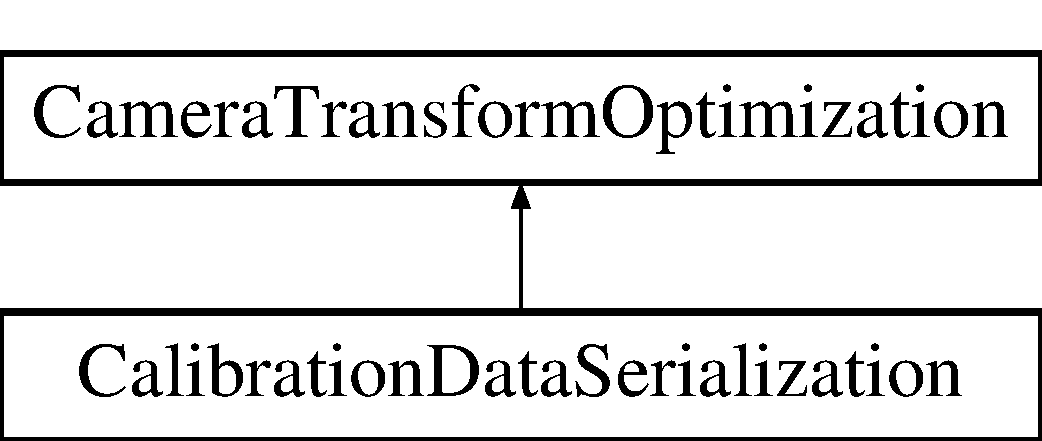
\includegraphics[height=2.000000cm]{classCalibrationDataSerialization}
\end{center}
\end{figure}
\subsection*{\-Public \-Member \-Functions}
\begin{DoxyCompactItemize}
\item 
\hypertarget{classCalibrationDataSerialization_abcc65d6c8575184b85167bb078e4e4df}{{\bfseries \-Calibration\-Data\-Serialization} (\hyperlink{classDataCaptureParameter}{\-Data\-Capture\-Parameter} data\-Capture\-Parameter, std\-::string filename)}\label{classCalibrationDataSerialization_abcc65d6c8575184b85167bb078e4e4df}

\item 
virtual void \hyperlink{classCalibrationDataSerialization_a7e7db9387843500002e908cb54a0b5ea}{optimize\-Transform} (\hyperlink{classCalibrationState}{\-Calibration\-State} \&calibration\-State)
\item 
\hypertarget{classCalibrationDataSerialization_ad3475e1d828cfd3a32f8de89b85f6a25}{virtual std\-::vector$<$ \hyperlink{classCameraMeasurePoint}{\-Measure\-Point} $>$ {\bfseries get\-Measurement\-Series} ()}\label{classCalibrationDataSerialization_ad3475e1d828cfd3a32f8de89b85f6a25}

\item 
\hypertarget{classCalibrationDataSerialization_afd543f2bf35bda0f5b2b6017df2374d3}{virtual tf\-::\-Transform {\bfseries get\-Initial\-Transform} ()}\label{classCalibrationDataSerialization_afd543f2bf35bda0f5b2b6017df2374d3}

\end{DoxyCompactItemize}
\subsection*{\-Protected \-Member \-Functions}
\begin{DoxyCompactItemize}
\item 
\hypertarget{classCalibrationDataSerialization_a943de2495acf5373c4dab9adcbbc4df9}{void {\bfseries save\-To\-File} ()}\label{classCalibrationDataSerialization_a943de2495acf5373c4dab9adcbbc4df9}

\item 
\hypertarget{classCalibrationDataSerialization_ac4f52c834c9a2e60533b3e95f492a40e}{void {\bfseries load\-From\-File} ()}\label{classCalibrationDataSerialization_ac4f52c834c9a2e60533b3e95f492a40e}

\end{DoxyCompactItemize}


\subsection{\-Member \-Function \-Documentation}
\hypertarget{classCalibrationDataSerialization_a7e7db9387843500002e908cb54a0b5ea}{\index{\-Calibration\-Data\-Serialization@{\-Calibration\-Data\-Serialization}!optimize\-Transform@{optimize\-Transform}}
\index{optimize\-Transform@{optimize\-Transform}!CalibrationDataSerialization@{\-Calibration\-Data\-Serialization}}
\subsubsection[{optimize\-Transform}]{\setlength{\rightskip}{0pt plus 5cm}void {\bf \-Calibration\-Data\-Serialization\-::optimize\-Transform} (
\begin{DoxyParamCaption}
\item[{{\bf \-Calibration\-State} \&}]{calibration\-State}
\end{DoxyParamCaption}
)\hspace{0.3cm}{\ttfamily  \mbox{[}virtual\mbox{]}}}}\label{classCalibrationDataSerialization_a7e7db9387843500002e908cb54a0b5ea}
\-Optimizes the transform given the measured points, initial transformation, and all other transformations needed. 

\-Implements \hyperlink{classCameraTransformOptimization_a8a4a4a09325f4bae401bad62ec7e9f02}{\-Camera\-Transform\-Optimization}.



\-The documentation for this class was generated from the following files\-:\begin{DoxyCompactItemize}
\item 
/home/stefan/catkin\-\_\-ws/src/calibration/include/\-Calibration\-Data\-Serialization.\-h\item 
/home/stefan/catkin\-\_\-ws/src/calibration/src/\-Calibration\-Data\-Serialization.\-cpp\end{DoxyCompactItemize}

\hypertarget{classCalibrationState}{\section{\-Calibration\-State \-Class \-Reference}
\label{classCalibrationState}\index{\-Calibration\-State@{\-Calibration\-State}}
}
\-Inheritance diagram for \-Calibration\-State\-:\begin{figure}[H]
\begin{center}
\leavevmode
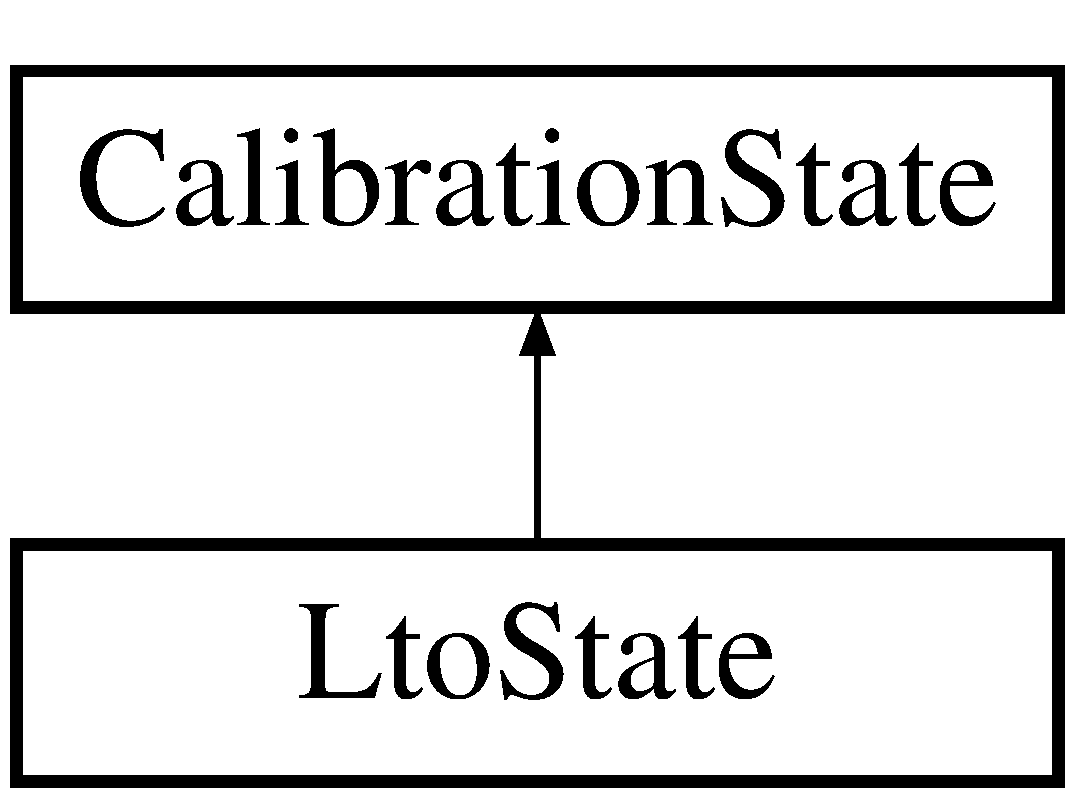
\includegraphics[height=2.000000cm]{classCalibrationState}
\end{center}
\end{figure}
\subsection*{\-Public \-Member \-Functions}
\begin{DoxyCompactItemize}
\item 
\hypertarget{classCalibrationState_a7002f5f76f264c02f739f0ace6111b42}{{\bfseries \-Calibration\-State} (tf\-::\-Transform camera\-To\-Head, double head\-Yaw\-Offset, double head\-Pitch\-Offset)}\label{classCalibrationState_a7002f5f76f264c02f739f0ace6111b42}

\item 
\hypertarget{classCalibrationState_a099c6593f5ec4addd6f20e493abcbad8}{tf\-::\-Transform {\bfseries get\-Camera\-To\-Head} () const }\label{classCalibrationState_a099c6593f5ec4addd6f20e493abcbad8}

\item 
\hypertarget{classCalibrationState_aa2872b95786b896a3bd3bdaf6835cbde}{void {\bfseries set\-Camera\-To\-Head} (const tf\-::\-Transform \&camera\-To\-Head)}\label{classCalibrationState_aa2872b95786b896a3bd3bdaf6835cbde}

\item 
\hypertarget{classCalibrationState_a15355c0a9e96021d0910b6f05c5ed182}{double {\bfseries get\-Head\-Pitch\-Offset} () const }\label{classCalibrationState_a15355c0a9e96021d0910b6f05c5ed182}

\item 
\hypertarget{classCalibrationState_a0575b632bdf3e6491867aeba5656f42f}{void {\bfseries set\-Head\-Pitch\-Offset} (double head\-Pitch\-Offset)}\label{classCalibrationState_a0575b632bdf3e6491867aeba5656f42f}

\item 
\hypertarget{classCalibrationState_ad44ffdadc1c02f4a7bb25ae80acfb974}{double {\bfseries get\-Head\-Yaw\-Offset} () const }\label{classCalibrationState_ad44ffdadc1c02f4a7bb25ae80acfb974}

\item 
\hypertarget{classCalibrationState_a379d025cd3dff837a89620137dda3919}{void {\bfseries set\-Head\-Yaw\-Offset} (double head\-Yaw\-Offset)}\label{classCalibrationState_a379d025cd3dff837a89620137dda3919}

\end{DoxyCompactItemize}
\subsection*{\-Protected \-Attributes}
\begin{DoxyCompactItemize}
\item 
\hypertarget{classCalibrationState_ab392422f78f1886a9c04d5c0a4bc6464}{tf\-::\-Transform {\bfseries camera\-To\-Head}}\label{classCalibrationState_ab392422f78f1886a9c04d5c0a4bc6464}

\item 
\hypertarget{classCalibrationState_a59e5973fd377639de9bf5f854e3ee575}{double {\bfseries head\-Yaw\-Offset}}\label{classCalibrationState_a59e5973fd377639de9bf5f854e3ee575}

\item 
\hypertarget{classCalibrationState_adabafa1ab274107017ce2daadeb45b44}{double {\bfseries head\-Pitch\-Offset}}\label{classCalibrationState_adabafa1ab274107017ce2daadeb45b44}

\end{DoxyCompactItemize}


\-The documentation for this class was generated from the following files\-:\begin{DoxyCompactItemize}
\item 
/home/stefan/catkin\-\_\-ws/src/calibration/include/\-Calibration\-State.\-h\item 
/home/stefan/catkin\-\_\-ws/src/calibration/src/\-Calibration\-State.\-cpp\end{DoxyCompactItemize}

\hypertarget{classCameraCalibration}{\section{\-Camera\-Calibration \-Class \-Reference}
\label{classCameraCalibration}\index{\-Camera\-Calibration@{\-Camera\-Calibration}}
}
\subsection*{\-Public \-Member \-Functions}
\begin{DoxyCompactItemize}
\item 
\hypertarget{classCameraCalibration_adadb438daab6669517b1bc617676529d}{{\bfseries \-Camera\-Calibration} (\hyperlink{classCameraCalibrationOptions}{\-Camera\-Calibration\-Options} options)}\label{classCameraCalibration_adadb438daab6669517b1bc617676529d}

\item 
\hypertarget{classCameraCalibration_af7a69e0088701c48242b375c9e4cd7e0}{void {\bfseries start\-Optimization} ()}\label{classCameraCalibration_af7a69e0088701c48242b375c9e4cd7e0}

\item 
\hypertarget{classCameraCalibration_a1d670d71bb381cd092115491edaf4dea}{void {\bfseries set\-Data} (std\-::vector$<$ \hyperlink{classCameraMeasurePoint}{\-Measure\-Point} $>$ measurement\-Series, tf\-::\-Transform initial\-Transform)}\label{classCameraCalibration_a1d670d71bb381cd092115491edaf4dea}

\item 
\hypertarget{classCameraCalibration_a2a4c7aa5a6adcfc88d0d2537e31640c9}{void {\bfseries start\-Loop} ()}\label{classCameraCalibration_a2a4c7aa5a6adcfc88d0d2537e31640c9}

\item 
\hypertarget{classCameraCalibration_afa9ebb2c505f52ffe92954c1a50b6227}{const \hyperlink{classCameraTransformOptimization}{\-Camera\-Transform\-Optimization} $\ast$ {\bfseries get\-Transform\-Optimization} () const }\label{classCameraCalibration_afa9ebb2c505f52ffe92954c1a50b6227}

\item 
\hypertarget{classCameraCalibration_aca396b1f90004b521b7716f9ca303c80}{void {\bfseries set\-Transform\-Optimization} (\hyperlink{classCameraTransformOptimization}{\-Camera\-Transform\-Optimization} $\ast$transform\-Optimization)}\label{classCameraCalibration_aca396b1f90004b521b7716f9ca303c80}

\end{DoxyCompactItemize}
\subsection*{\-Protected \-Member \-Functions}
\begin{DoxyCompactItemize}
\item 
\hypertarget{classCameraCalibration_a73d0baadef762436150174cadb27a5aa}{void {\bfseries pointcloud\-Msg\-Cb} (const sensor\-\_\-msgs\-::\-Point\-Cloud2 \&input)}\label{classCameraCalibration_a73d0baadef762436150174cadb27a5aa}

\item 
\hypertarget{classCameraCalibration_aeaae564e9b82a15efe553efb6ba627a6}{void {\bfseries setup\-Terminal} ()}\label{classCameraCalibration_aeaae564e9b82a15efe553efb6ba627a6}

\item 
\hypertarget{classCameraCalibration_a2b4033f9d559a82cee68237c0b8c2bd7}{void {\bfseries restore\-Terminal} ()}\label{classCameraCalibration_a2b4033f9d559a82cee68237c0b8c2bd7}

\item 
\hypertarget{classCameraCalibration_ae351fadc3fec0f192685100374a5558d}{void {\bfseries spin\-Once} ()}\label{classCameraCalibration_ae351fadc3fec0f192685100374a5558d}

\item 
\hypertarget{classCameraCalibration_a2a687bb66def89d06def28abb889ce40}{void {\bfseries print\-Help} ()}\label{classCameraCalibration_a2a687bb66def89d06def28abb889ce40}

\end{DoxyCompactItemize}


\-The documentation for this class was generated from the following files\-:\begin{DoxyCompactItemize}
\item 
/home/stefan/catkin\-\_\-ws/src/calibration/include/\-Camera\-Calibration.\-h\item 
/home/stefan/catkin\-\_\-ws/src/calibration/src/\-Camera\-Calibration.\-cpp\end{DoxyCompactItemize}

\hypertarget{classCameraCalibrationOptions}{\section{\-Camera\-Calibration\-Options \-Class \-Reference}
\label{classCameraCalibrationOptions}\index{\-Camera\-Calibration\-Options@{\-Camera\-Calibration\-Options}}
}
\subsection*{\-Public \-Member \-Functions}
\begin{DoxyCompactItemize}
\item 
\hypertarget{classCameraCalibrationOptions_a625eff0db9f89abe9007e5ea7937d701}{\hyperlink{classBallDetectionParameter}{\-Ball\-Detection\-Parameter} \& {\bfseries get\-Ball\-Detection\-Parameter} ()}\label{classCameraCalibrationOptions_a625eff0db9f89abe9007e5ea7937d701}

\item 
\hypertarget{classCameraCalibrationOptions_a995130e8d921df7698903c295bbf8329}{void {\bfseries set\-Ball\-Detection\-Parameter} (const \hyperlink{classBallDetectionParameter}{\-Ball\-Detection\-Parameter} \&ball\-Detection\-Parameter)}\label{classCameraCalibrationOptions_a995130e8d921df7698903c295bbf8329}

\item 
\hypertarget{classCameraCalibrationOptions_a8d75416c4ff7f9b5d9dfc5d2bd75a39c}{\hyperlink{classDataCaptureParameter}{\-Data\-Capture\-Parameter} \& {\bfseries get\-Data\-Capture\-Parameter} ()}\label{classCameraCalibrationOptions_a8d75416c4ff7f9b5d9dfc5d2bd75a39c}

\item 
\hypertarget{classCameraCalibrationOptions_a553eae8fe71c597667e6055934dd4563}{void {\bfseries set\-Data\-Capture\-Parameter} (const \hyperlink{classDataCaptureParameter}{\-Data\-Capture\-Parameter} \&data\-Capture\-Parameter)}\label{classCameraCalibrationOptions_a553eae8fe71c597667e6055934dd4563}

\item 
\hypertarget{classCameraCalibrationOptions_a9a4406fd58f084f47d77d69c086f71ec}{std\-::vector\*
$<$ \hyperlink{classCameraTransformOptimizationParameter}{\-Camera\-Transform\-Optimization\-Parameter} $>$ \& {\bfseries get\-Camera\-Transform\-Optimization\-Parameter} ()}\label{classCameraCalibrationOptions_a9a4406fd58f084f47d77d69c086f71ec}

\item 
\hypertarget{classCameraCalibrationOptions_a487780fc6c9b0425411c21fcb084a464}{void {\bfseries set\-Camera\-Transform\-Optimization\-Parameter} (const std\-::vector$<$ \hyperlink{classCameraTransformOptimizationParameter}{\-Camera\-Transform\-Optimization\-Parameter} $>$ \&camera\-Transform\-Optimization\-Parameter)}\label{classCameraCalibrationOptions_a487780fc6c9b0425411c21fcb084a464}

\end{DoxyCompactItemize}
\subsection*{\-Protected \-Attributes}
\begin{DoxyCompactItemize}
\item 
\hypertarget{classCameraCalibrationOptions_ac4ce9c7aed964e8b7a4d7ed1ffae28ce}{std\-::vector\*
$<$ \hyperlink{classCameraTransformOptimizationParameter}{\-Camera\-Transform\-Optimization\-Parameter} $>$ {\bfseries camera\-Transform\-Optimization\-Parameter}}\label{classCameraCalibrationOptions_ac4ce9c7aed964e8b7a4d7ed1ffae28ce}

\item 
\hypertarget{classCameraCalibrationOptions_a8a4c1bafb4c1d402c0a6770db93f8189}{\hyperlink{classBallDetectionParameter}{\-Ball\-Detection\-Parameter} {\bfseries ball\-Detection\-Parameter}}\label{classCameraCalibrationOptions_a8a4c1bafb4c1d402c0a6770db93f8189}

\item 
\hypertarget{classCameraCalibrationOptions_a2f288866a304a47821e8a6b3af90ab2a}{\hyperlink{classDataCaptureParameter}{\-Data\-Capture\-Parameter} {\bfseries data\-Capture\-Parameter}}\label{classCameraCalibrationOptions_a2f288866a304a47821e8a6b3af90ab2a}

\end{DoxyCompactItemize}


\-The documentation for this class was generated from the following file\-:\begin{DoxyCompactItemize}
\item 
/home/stefan/catkin\-\_\-ws/src/calibration/include/\-Parameter.\-h\end{DoxyCompactItemize}

\hypertarget{classCameraMeasurePoint}{\section{\-Camera\-Measure\-Point \-Class \-Reference}
\label{classCameraMeasurePoint}\index{\-Camera\-Measure\-Point@{\-Camera\-Measure\-Point}}
}
\subsection*{\-Public \-Member \-Functions}
\begin{DoxyCompactItemize}
\item 
\hyperlink{classCameraMeasurePoint}{\-Camera\-Measure\-Point} \hyperlink{classCameraMeasurePoint_a86e386600a98acad86f70a5aa4d895ce}{with\-Head\-Yaw\-Offset} (double head\-Yaw\-Offset)
\item 
\hyperlink{classCameraMeasurePoint}{\-Camera\-Measure\-Point} \hyperlink{classCameraMeasurePoint_ab1ff9ca0a9fc47aa6e943e93b513eda7}{with\-Head\-Pitch\-Offset} (double head\-Pitch\-Offset)
\item 
\hypertarget{classCameraMeasurePoint_ad2b821cf3a179c25a039e5bf3e5696bc}{const tf\-::\-Transform {\bfseries head\-To\-Footprint} (const \hyperlink{classCalibrationState}{\-Calibration\-State} \&state) const }\label{classCameraMeasurePoint_ad2b821cf3a179c25a039e5bf3e5696bc}

\item 
\hypertarget{classCameraMeasurePoint_a7b82b2a1d296f878f27d9a459b7a158f}{const tf\-::\-Transform {\bfseries head\-To\-Fixed} (const \hyperlink{classCalibrationState}{\-Calibration\-State} \&state) const }\label{classCameraMeasurePoint_a7b82b2a1d296f878f27d9a459b7a158f}

\item 
\hypertarget{classCameraMeasurePoint_a0b34bfdb160f35fac423012e0dd5a7cd}{const tf\-::\-Pose {\bfseries ground\-Pose} () const }\label{classCameraMeasurePoint_a0b34bfdb160f35fac423012e0dd5a7cd}

\item 
\hypertarget{classCameraMeasurePoint_ab8444ead826ed2658d5ff18067ed27ad}{const tf\-::\-Transform {\bfseries optical\-To\-Footprint} (const \hyperlink{classCalibrationState}{\-Calibration\-State} \&state) const }\label{classCameraMeasurePoint_ab8444ead826ed2658d5ff18067ed27ad}

\item 
\hypertarget{classCameraMeasurePoint_a74a525a0c6bcb7f0ec8b67a758ded39b}{const tf\-::\-Transform {\bfseries optical\-To\-Fixed} (const \hyperlink{classCalibrationState}{\-Calibration\-State} \&state) const }\label{classCameraMeasurePoint_a74a525a0c6bcb7f0ec8b67a758ded39b}

\item 
\hypertarget{classCameraMeasurePoint_a940011f76fd6f61693cb4f0103318278}{const tf\-::\-Transform \& {\bfseries get\-Fixed\-To\-Footprint} () const }\label{classCameraMeasurePoint_a940011f76fd6f61693cb4f0103318278}

\item 
\hypertarget{classCameraMeasurePoint_a57a334748d902d8e4360770297599999}{void {\bfseries set\-Fixed\-To\-Footprint} (const tf\-::\-Transform \&fixed\-To\-Footprint)}\label{classCameraMeasurePoint_a57a334748d902d8e4360770297599999}

\item 
\hypertarget{classCameraMeasurePoint_a8b09fee300825cd0ea98a31ecbbf9a03}{const tf\-::\-Transform \& {\bfseries get\-Head\-Pitch\-To\-Head\-Yaw} () const }\label{classCameraMeasurePoint_a8b09fee300825cd0ea98a31ecbbf9a03}

\item 
\hypertarget{classCameraMeasurePoint_a268d759e6e173e10915b81dab304f830}{void {\bfseries set\-Head\-Pitch\-To\-Head\-Yaw} (const tf\-::\-Transform \&head\-Pitch\-To\-Head\-Yaw)}\label{classCameraMeasurePoint_a268d759e6e173e10915b81dab304f830}

\item 
\hypertarget{classCameraMeasurePoint_aa8e97a6061ee2d23d4ebd4078bf114b5}{const tf\-::\-Transform \& {\bfseries get\-Head\-Yaw\-To\-Torso} () const }\label{classCameraMeasurePoint_aa8e97a6061ee2d23d4ebd4078bf114b5}

\item 
\hypertarget{classCameraMeasurePoint_a3a13348fd95baef71d0ec49032856c2c}{void {\bfseries set\-Head\-Yaw\-To\-Torso} (const tf\-::\-Transform \&head\-Yaw\-To\-Torso)}\label{classCameraMeasurePoint_a3a13348fd95baef71d0ec49032856c2c}

\item 
\hypertarget{classCameraMeasurePoint_abf729566f8c54ae01a3d468fea94be32}{const tf\-::\-Transform \& {\bfseries get\-Optical\-To\-Camera} () const }\label{classCameraMeasurePoint_abf729566f8c54ae01a3d468fea94be32}

\item 
\hypertarget{classCameraMeasurePoint_a0652acb77f7e874dfdaad23a3652ce34}{void {\bfseries set\-Optical\-To\-Camera} (const tf\-::\-Transform \&optical\-To\-Camera)}\label{classCameraMeasurePoint_a0652acb77f7e874dfdaad23a3652ce34}

\item 
\hypertarget{classCameraMeasurePoint_a5b51d162cf7e23c684d0f36742ee6be9}{const tf\-::\-Transform \& {\bfseries get\-Torso\-To\-Fixed} () const }\label{classCameraMeasurePoint_a5b51d162cf7e23c684d0f36742ee6be9}

\item 
\hypertarget{classCameraMeasurePoint_a2a5c35e0cc027ee7ef20803fa8047e7c}{void {\bfseries set\-Torso\-To\-Fixed} (const tf\-::\-Transform \&torso\-To\-Fixed)}\label{classCameraMeasurePoint_a2a5c35e0cc027ee7ef20803fa8047e7c}

\end{DoxyCompactItemize}
\subsection*{\-Public \-Attributes}
\begin{DoxyCompactItemize}
\item 
\hypertarget{classCameraMeasurePoint_a5c2735947cad152b61ee5a5533f10e93}{tf\-::\-Vector3 {\bfseries measured\-Position}}\label{classCameraMeasurePoint_a5c2735947cad152b61ee5a5533f10e93}

\item 
\hypertarget{classCameraMeasurePoint_a33ba739473857149068b5a4529278539}{\hyperlink{classGroundData}{\-Ground\-Data} {\bfseries ground\-Data}}\label{classCameraMeasurePoint_a33ba739473857149068b5a4529278539}

\item 
\hypertarget{classCameraMeasurePoint_a6f1026a96880cbafc51eaf3461342ae4}{ros\-::\-Time {\bfseries stamp}}\label{classCameraMeasurePoint_a6f1026a96880cbafc51eaf3461342ae4}

\end{DoxyCompactItemize}
\subsection*{\-Friends}
\begin{DoxyCompactItemize}
\item 
\hypertarget{classCameraMeasurePoint_aca7ee4caa1a60efd63c2108f8b0e813c}{ostream \& {\bfseries operator$<$$<$} (ostream \&output, const \hyperlink{classCameraMeasurePoint}{\-Camera\-Measure\-Point} \&cmp)}\label{classCameraMeasurePoint_aca7ee4caa1a60efd63c2108f8b0e813c}

\item 
\hypertarget{classCameraMeasurePoint_ab4e8c4560da3882efc55092c741e1d2f}{istream \& {\bfseries operator$>$$>$} (istream \&input, \hyperlink{classCameraMeasurePoint}{\-Camera\-Measure\-Point} \&cmp)}\label{classCameraMeasurePoint_ab4e8c4560da3882efc55092c741e1d2f}

\end{DoxyCompactItemize}


\subsection{\-Member \-Function \-Documentation}
\hypertarget{classCameraMeasurePoint_ab1ff9ca0a9fc47aa6e943e93b513eda7}{\index{\-Camera\-Measure\-Point@{\-Camera\-Measure\-Point}!with\-Head\-Pitch\-Offset@{with\-Head\-Pitch\-Offset}}
\index{with\-Head\-Pitch\-Offset@{with\-Head\-Pitch\-Offset}!CameraMeasurePoint@{\-Camera\-Measure\-Point}}
\subsubsection[{with\-Head\-Pitch\-Offset}]{\setlength{\rightskip}{0pt plus 5cm}{\bf \-Camera\-Measure\-Point} {\bf \-Camera\-Measure\-Point\-::with\-Head\-Pitch\-Offset} (
\begin{DoxyParamCaption}
\item[{double}]{head\-Pitch\-Offset}
\end{DoxyParamCaption}
)}}\label{classCameraMeasurePoint_ab1ff9ca0a9fc47aa6e943e93b513eda7}
\-Returns the measure point with an offset set to the \-Head\-Pitch joint \hypertarget{classCameraMeasurePoint_a86e386600a98acad86f70a5aa4d895ce}{\index{\-Camera\-Measure\-Point@{\-Camera\-Measure\-Point}!with\-Head\-Yaw\-Offset@{with\-Head\-Yaw\-Offset}}
\index{with\-Head\-Yaw\-Offset@{with\-Head\-Yaw\-Offset}!CameraMeasurePoint@{\-Camera\-Measure\-Point}}
\subsubsection[{with\-Head\-Yaw\-Offset}]{\setlength{\rightskip}{0pt plus 5cm}{\bf \-Camera\-Measure\-Point} {\bf \-Camera\-Measure\-Point\-::with\-Head\-Yaw\-Offset} (
\begin{DoxyParamCaption}
\item[{double}]{head\-Yaw\-Offset}
\end{DoxyParamCaption}
)}}\label{classCameraMeasurePoint_a86e386600a98acad86f70a5aa4d895ce}
\-Returns the measure point with an offset set to the \-Head\-Yaw joint 

\-The documentation for this class was generated from the following files\-:\begin{DoxyCompactItemize}
\item 
/home/stefan/catkin\-\_\-ws/src/calibration/include/\-Camera\-Measure\-Point.\-h\item 
/home/stefan/catkin\-\_\-ws/src/calibration/src/\-Camera\-Measure\-Point.\-cpp\end{DoxyCompactItemize}

\hypertarget{classCameraTransformOptimization}{\section{\-Camera\-Transform\-Optimization \-Class \-Reference}
\label{classCameraTransformOptimization}\index{\-Camera\-Transform\-Optimization@{\-Camera\-Transform\-Optimization}}
}
\-Inheritance diagram for \-Camera\-Transform\-Optimization\-:\begin{figure}[H]
\begin{center}
\leavevmode
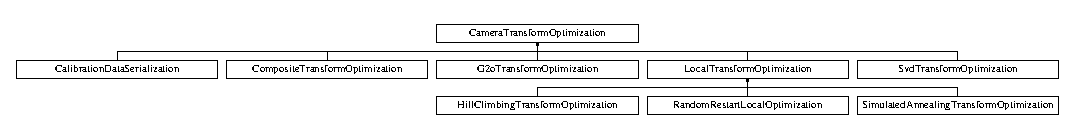
\includegraphics[height=1.312500cm]{classCameraTransformOptimization}
\end{center}
\end{figure}
\subsection*{\-Public \-Member \-Functions}
\begin{DoxyCompactItemize}
\item 
\hyperlink{classCameraTransformOptimization_a8c184b6dd5e2db624109d76ffb90c026}{\-Camera\-Transform\-Optimization} (\hyperlink{classCameraTransformOptimizationParameter}{\-Camera\-Transform\-Optimization\-Parameter} parameter=\hyperlink{classCameraTransformOptimizationParameter}{\-Camera\-Transform\-Optimization\-Parameter}())
\item 
virtual \hyperlink{classCameraTransformOptimization_a1d34a5b00c8222fac7e5939f88f55e96}{$\sim$\-Camera\-Transform\-Optimization} ()
\item 
virtual void \hyperlink{classCameraTransformOptimization_a8a4a4a09325f4bae401bad62ec7e9f02}{optimize\-Transform} (\hyperlink{classCalibrationState}{\-Calibration\-State} \&calibration\-State)=0
\item 
virtual void \hyperlink{classCameraTransformOptimization_ac1ffbf2ddfc7e7de7639e870d0745957}{add\-Measure\-Point} (\hyperlink{classCameraMeasurePoint}{\-Measure\-Point} new\-Point)
\item 
virtual void \hyperlink{classCameraTransformOptimization_a53007c5c531dd86a5facf7cbc82f477e}{clear\-Measure\-Points} ()
\item 
virtual void \hyperlink{classCameraTransformOptimization_abdd025826d3ece8861c07d91fa5cb98e}{calculate\-Sqrt\-Dist\-From\-Marker} (\hyperlink{classCalibrationState}{\-Calibration\-State} state, tf\-::\-Vector3 marker\-Point, float \&error)
\item 
virtual void \hyperlink{classCameraTransformOptimization_ae23b52f59e2f4eb5e37eca8ba0e3fc1b}{calculate\-Sqrt\-Dist\-Camera\-Head} (tf\-::\-Transform camera\-To\-Head, float \&error)
\item 
virtual void \hyperlink{classCameraTransformOptimization_a63da0977758e7a4b63f946ada33e7dd5}{get\-Marker\-Estimate} (const \hyperlink{classCalibrationState}{\-Calibration\-State} \&camera\-To\-Head, tf\-::\-Vector3 \&position)
\item 
void \hyperlink{classCameraTransformOptimization_a2ac72c140004cc3b2259ef4d2438cafb}{print\-Result} (std\-::string pre, const \hyperlink{classCalibrationState}{\-Calibration\-State} \&camera\-To\-Head, tf\-::\-Vector3 marker\-Position)
\item 
void \hyperlink{classCameraTransformOptimization_a913127f90c84a4e4505b057939280f89}{get\-Avg\-R\-P} (const \hyperlink{classCalibrationState}{\-Calibration\-State} \&state, double \&r, double \&p)
\item 
\hypertarget{classCameraTransformOptimization_af11daaf2cd5178c7fe4d0596a9f544de}{virtual void {\bfseries remove\-Outliers} ()}\label{classCameraTransformOptimization_af11daaf2cd5178c7fe4d0596a9f544de}

\item 
\hypertarget{classCameraTransformOptimization_ac9e55b35f8ee89aff5bb3d33301f420f}{int {\bfseries get\-Max\-Iterations} () const }\label{classCameraTransformOptimization_ac9e55b35f8ee89aff5bb3d33301f420f}

\item 
\hypertarget{classCameraTransformOptimization_a04ea90d9c105f077afad21d88a3cddc4}{void {\bfseries set\-Max\-Iterations} (int max\-Iterations)}\label{classCameraTransformOptimization_a04ea90d9c105f077afad21d88a3cddc4}

\item 
\hypertarget{classCameraTransformOptimization_af4e92403855d44d3abb3d81a33ea3be9}{float {\bfseries get\-Min\-Error} () const }\label{classCameraTransformOptimization_af4e92403855d44d3abb3d81a33ea3be9}

\item 
\hypertarget{classCameraTransformOptimization_a2bc589d6107bde5c4c9485cc40df2693}{void {\bfseries set\-Min\-Error} (float min\-Error)}\label{classCameraTransformOptimization_a2bc589d6107bde5c4c9485cc40df2693}

\item 
\hypertarget{classCameraTransformOptimization_ae46ae0f7bf817dc0f1cd1528f3e40a40}{float {\bfseries get\-Error\-Improvement} () const }\label{classCameraTransformOptimization_ae46ae0f7bf817dc0f1cd1528f3e40a40}

\item 
\hypertarget{classCameraTransformOptimization_a0234fcab0dea261cc3c998af4a95a76a}{void {\bfseries set\-Error\-Improvement} (float error\-Improvement)}\label{classCameraTransformOptimization_a0234fcab0dea261cc3c998af4a95a76a}

\item 
\hypertarget{classCameraTransformOptimization_a5cd1ad3be856ba781dd5ce7a29ae3401}{virtual tf\-::\-Transform {\bfseries get\-Initial\-Camera\-To\-Head} ()}\label{classCameraTransformOptimization_a5cd1ad3be856ba781dd5ce7a29ae3401}

\item 
\hypertarget{classCameraTransformOptimization_a3e576d28d6fce0310bb35aa03e9d1223}{virtual void {\bfseries set\-Initial\-Camera\-To\-Head} (tf\-::\-Transform initial\-Transform)}\label{classCameraTransformOptimization_a3e576d28d6fce0310bb35aa03e9d1223}

\end{DoxyCompactItemize}
\subsection*{\-Protected \-Member \-Functions}
\begin{DoxyCompactItemize}
\item 
\hypertarget{classCameraTransformOptimization_a51edcef959641febc34e4191e049acf3}{virtual bool {\bfseries can\-Stop} ()}\label{classCameraTransformOptimization_a51edcef959641febc34e4191e049acf3}

\end{DoxyCompactItemize}
\subsection*{\-Protected \-Attributes}
\begin{DoxyCompactItemize}
\item 
\hypertarget{classCameraTransformOptimization_abd78313124b14d012b208794942d2052}{int {\bfseries num\-Of\-Iterations}}\label{classCameraTransformOptimization_abd78313124b14d012b208794942d2052}

\item 
\hypertarget{classCameraTransformOptimization_a245be304c2a3c477fbedb7f467e76a92}{std\-::vector$<$ \hyperlink{classCameraMeasurePoint}{\-Measure\-Point} $>$ {\bfseries measure\-Points}}\label{classCameraTransformOptimization_a245be304c2a3c477fbedb7f467e76a92}

\item 
\hypertarget{classCameraTransformOptimization_ae07e112f39b9fa85b84055d9b859366d}{float {\bfseries error}}\label{classCameraTransformOptimization_ae07e112f39b9fa85b84055d9b859366d}

\item 
\hypertarget{classCameraTransformOptimization_aa250b60379325fa6a535e3defda4003f}{float {\bfseries last\-Error}}\label{classCameraTransformOptimization_aa250b60379325fa6a535e3defda4003f}

\item 
\hypertarget{classCameraTransformOptimization_a201614fd0ce051b2a407d8cc66efbf08}{float {\bfseries error\-Improvement}}\label{classCameraTransformOptimization_a201614fd0ce051b2a407d8cc66efbf08}

\item 
\hypertarget{classCameraTransformOptimization_a998dd4ef202d17047b05ca5b90ab5553}{float {\bfseries min\-Error}}\label{classCameraTransformOptimization_a998dd4ef202d17047b05ca5b90ab5553}

\item 
\hypertarget{classCameraTransformOptimization_a75230bc2bb1f6d7336ac6a3bf568a805}{int {\bfseries max\-Iterations}}\label{classCameraTransformOptimization_a75230bc2bb1f6d7336ac6a3bf568a805}

\item 
\hypertarget{classCameraTransformOptimization_a6f4d4dd70f728d94f6da1d18da5e309e}{\hyperlink{classCameraTransformOptimizationParameter}{\-Camera\-Transform\-Optimization\-Parameter} {\bfseries parameter}}\label{classCameraTransformOptimization_a6f4d4dd70f728d94f6da1d18da5e309e}

\end{DoxyCompactItemize}


\subsection{\-Constructor \& \-Destructor \-Documentation}
\hypertarget{classCameraTransformOptimization_a8c184b6dd5e2db624109d76ffb90c026}{\index{\-Camera\-Transform\-Optimization@{\-Camera\-Transform\-Optimization}!\-Camera\-Transform\-Optimization@{\-Camera\-Transform\-Optimization}}
\index{\-Camera\-Transform\-Optimization@{\-Camera\-Transform\-Optimization}!CameraTransformOptimization@{\-Camera\-Transform\-Optimization}}
\subsubsection[{\-Camera\-Transform\-Optimization}]{\setlength{\rightskip}{0pt plus 5cm}{\bf \-Camera\-Transform\-Optimization\-::\-Camera\-Transform\-Optimization} (
\begin{DoxyParamCaption}
\item[{{\bf \-Camera\-Transform\-Optimization\-Parameter}}]{parameter = {\ttfamily {\bf \-Camera\-Transform\-Optimization\-Parameter}()}}
\end{DoxyParamCaption}
)}}\label{classCameraTransformOptimization_a8c184b6dd5e2db624109d76ffb90c026}
\-Parameterized constructor. \hypertarget{classCameraTransformOptimization_a1d34a5b00c8222fac7e5939f88f55e96}{\index{\-Camera\-Transform\-Optimization@{\-Camera\-Transform\-Optimization}!$\sim$\-Camera\-Transform\-Optimization@{$\sim$\-Camera\-Transform\-Optimization}}
\index{$\sim$\-Camera\-Transform\-Optimization@{$\sim$\-Camera\-Transform\-Optimization}!CameraTransformOptimization@{\-Camera\-Transform\-Optimization}}
\subsubsection[{$\sim$\-Camera\-Transform\-Optimization}]{\setlength{\rightskip}{0pt plus 5cm}{\bf \-Camera\-Transform\-Optimization\-::$\sim$\-Camera\-Transform\-Optimization} (
\begin{DoxyParamCaption}
{}
\end{DoxyParamCaption}
)\hspace{0.3cm}{\ttfamily  \mbox{[}virtual\mbox{]}}}}\label{classCameraTransformOptimization_a1d34a5b00c8222fac7e5939f88f55e96}
\-Deconstructor. 

\subsection{\-Member \-Function \-Documentation}
\hypertarget{classCameraTransformOptimization_ac1ffbf2ddfc7e7de7639e870d0745957}{\index{\-Camera\-Transform\-Optimization@{\-Camera\-Transform\-Optimization}!add\-Measure\-Point@{add\-Measure\-Point}}
\index{add\-Measure\-Point@{add\-Measure\-Point}!CameraTransformOptimization@{\-Camera\-Transform\-Optimization}}
\subsubsection[{add\-Measure\-Point}]{\setlength{\rightskip}{0pt plus 5cm}void {\bf \-Camera\-Transform\-Optimization\-::add\-Measure\-Point} (
\begin{DoxyParamCaption}
\item[{{\bf \-Measure\-Point}}]{new\-Point}
\end{DoxyParamCaption}
)\hspace{0.3cm}{\ttfamily  \mbox{[}virtual\mbox{]}}}}\label{classCameraTransformOptimization_ac1ffbf2ddfc7e7de7639e870d0745957}
\-Adds a new measure point. 

\-Reimplemented in \hyperlink{classCompositeTransformOptimization_aff2a0c0afce22998d1a1128b1671d99c}{\-Composite\-Transform\-Optimization}.

\hypertarget{classCameraTransformOptimization_ae23b52f59e2f4eb5e37eca8ba0e3fc1b}{\index{\-Camera\-Transform\-Optimization@{\-Camera\-Transform\-Optimization}!calculate\-Sqrt\-Dist\-Camera\-Head@{calculate\-Sqrt\-Dist\-Camera\-Head}}
\index{calculate\-Sqrt\-Dist\-Camera\-Head@{calculate\-Sqrt\-Dist\-Camera\-Head}!CameraTransformOptimization@{\-Camera\-Transform\-Optimization}}
\subsubsection[{calculate\-Sqrt\-Dist\-Camera\-Head}]{\setlength{\rightskip}{0pt plus 5cm}void {\bf \-Camera\-Transform\-Optimization\-::calculate\-Sqrt\-Dist\-Camera\-Head} (
\begin{DoxyParamCaption}
\item[{tf\-::\-Transform}]{camera\-To\-Head, }
\item[{float \&}]{error}
\end{DoxyParamCaption}
)\hspace{0.3cm}{\ttfamily  \mbox{[}virtual\mbox{]}}}}\label{classCameraTransformOptimization_ae23b52f59e2f4eb5e37eca8ba0e3fc1b}
\-Calculates the error between the point clouds in the first camera frame and the transformed points in the last robot frame. \hypertarget{classCameraTransformOptimization_abdd025826d3ece8861c07d91fa5cb98e}{\index{\-Camera\-Transform\-Optimization@{\-Camera\-Transform\-Optimization}!calculate\-Sqrt\-Dist\-From\-Marker@{calculate\-Sqrt\-Dist\-From\-Marker}}
\index{calculate\-Sqrt\-Dist\-From\-Marker@{calculate\-Sqrt\-Dist\-From\-Marker}!CameraTransformOptimization@{\-Camera\-Transform\-Optimization}}
\subsubsection[{calculate\-Sqrt\-Dist\-From\-Marker}]{\setlength{\rightskip}{0pt plus 5cm}void {\bf \-Camera\-Transform\-Optimization\-::calculate\-Sqrt\-Dist\-From\-Marker} (
\begin{DoxyParamCaption}
\item[{{\bf \-Calibration\-State}}]{state, }
\item[{tf\-::\-Vector3}]{marker\-Point, }
\item[{float \&}]{error}
\end{DoxyParamCaption}
)\hspace{0.3cm}{\ttfamily  \mbox{[}virtual\mbox{]}}}}\label{classCameraTransformOptimization_abdd025826d3ece8861c07d91fa5cb98e}
\-Calculates the squared distance from the estimated marker position and the measured points given the current estimation for the transformation. \hypertarget{classCameraTransformOptimization_a53007c5c531dd86a5facf7cbc82f477e}{\index{\-Camera\-Transform\-Optimization@{\-Camera\-Transform\-Optimization}!clear\-Measure\-Points@{clear\-Measure\-Points}}
\index{clear\-Measure\-Points@{clear\-Measure\-Points}!CameraTransformOptimization@{\-Camera\-Transform\-Optimization}}
\subsubsection[{clear\-Measure\-Points}]{\setlength{\rightskip}{0pt plus 5cm}void {\bf \-Camera\-Transform\-Optimization\-::clear\-Measure\-Points} (
\begin{DoxyParamCaption}
{}
\end{DoxyParamCaption}
)\hspace{0.3cm}{\ttfamily  \mbox{[}virtual\mbox{]}}}}\label{classCameraTransformOptimization_a53007c5c531dd86a5facf7cbc82f477e}
\-Clears the list of measure points. 

\-Reimplemented in \hyperlink{classCompositeTransformOptimization_a5313f4fff02e5d48a7007af68ea6f008}{\-Composite\-Transform\-Optimization}.

\hypertarget{classCameraTransformOptimization_a913127f90c84a4e4505b057939280f89}{\index{\-Camera\-Transform\-Optimization@{\-Camera\-Transform\-Optimization}!get\-Avg\-R\-P@{get\-Avg\-R\-P}}
\index{get\-Avg\-R\-P@{get\-Avg\-R\-P}!CameraTransformOptimization@{\-Camera\-Transform\-Optimization}}
\subsubsection[{get\-Avg\-R\-P}]{\setlength{\rightskip}{0pt plus 5cm}void {\bf \-Camera\-Transform\-Optimization\-::get\-Avg\-R\-P} (
\begin{DoxyParamCaption}
\item[{const {\bf \-Calibration\-State} \&}]{state, }
\item[{double \&}]{r, }
\item[{double \&}]{p}
\end{DoxyParamCaption}
)}}\label{classCameraTransformOptimization_a913127f90c84a4e4505b057939280f89}
\-Calculates the average roll and pitch of the grond using the passed transformation. \hypertarget{classCameraTransformOptimization_a63da0977758e7a4b63f946ada33e7dd5}{\index{\-Camera\-Transform\-Optimization@{\-Camera\-Transform\-Optimization}!get\-Marker\-Estimate@{get\-Marker\-Estimate}}
\index{get\-Marker\-Estimate@{get\-Marker\-Estimate}!CameraTransformOptimization@{\-Camera\-Transform\-Optimization}}
\subsubsection[{get\-Marker\-Estimate}]{\setlength{\rightskip}{0pt plus 5cm}void {\bf \-Camera\-Transform\-Optimization\-::get\-Marker\-Estimate} (
\begin{DoxyParamCaption}
\item[{const {\bf \-Calibration\-State} \&}]{camera\-To\-Head, }
\item[{tf\-::\-Vector3 \&}]{position}
\end{DoxyParamCaption}
)\hspace{0.3cm}{\ttfamily  \mbox{[}virtual\mbox{]}}}}\label{classCameraTransformOptimization_a63da0977758e7a4b63f946ada33e7dd5}
\-Calculates an estimate for the marker position given a guess for the transformation. 

\-Reimplemented in \hyperlink{classG2oTransformOptimization_a2b3606f70377e7736712c131fe48d1ae}{\-G2o\-Transform\-Optimization}.

\hypertarget{classCameraTransformOptimization_a8a4a4a09325f4bae401bad62ec7e9f02}{\index{\-Camera\-Transform\-Optimization@{\-Camera\-Transform\-Optimization}!optimize\-Transform@{optimize\-Transform}}
\index{optimize\-Transform@{optimize\-Transform}!CameraTransformOptimization@{\-Camera\-Transform\-Optimization}}
\subsubsection[{optimize\-Transform}]{\setlength{\rightskip}{0pt plus 5cm}virtual void {\bf \-Camera\-Transform\-Optimization\-::optimize\-Transform} (
\begin{DoxyParamCaption}
\item[{{\bf \-Calibration\-State} \&}]{calibration\-State}
\end{DoxyParamCaption}
)\hspace{0.3cm}{\ttfamily  \mbox{[}pure virtual\mbox{]}}}}\label{classCameraTransformOptimization_a8a4a4a09325f4bae401bad62ec7e9f02}
\-Optimizes the transform given the measured points, initial transformation, and all other transformations needed. 

\-Implemented in \hyperlink{classCompositeTransformOptimization_aa77358fb8292c767bfbf029115ced9cf}{\-Composite\-Transform\-Optimization}, \hyperlink{classRandomRestartLocalOptimization_a6e5936d8717ed841becb50c1f04ee388}{\-Random\-Restart\-Local\-Optimization}, \hyperlink{classSimulatedAnnealingTransformOptimization_ab6690824306f9cd1f98f420a8d85e0f7}{\-Simulated\-Annealing\-Transform\-Optimization}, \hyperlink{classHillClimbingTransformOptimization_a4f7fb583e57929790420e1f28d97c383}{\-Hill\-Climbing\-Transform\-Optimization}, \hyperlink{classCalibrationDataSerialization_a7e7db9387843500002e908cb54a0b5ea}{\-Calibration\-Data\-Serialization}, \hyperlink{classG2oTransformOptimization_a8a644d4ab3d5cacd4cc56f716dfd648d}{\-G2o\-Transform\-Optimization}, and \hyperlink{classSvdTransformOptimization_afd4d0ed3de6c59535ede1f06134463e8}{\-Svd\-Transform\-Optimization}.

\hypertarget{classCameraTransformOptimization_a2ac72c140004cc3b2259ef4d2438cafb}{\index{\-Camera\-Transform\-Optimization@{\-Camera\-Transform\-Optimization}!print\-Result@{print\-Result}}
\index{print\-Result@{print\-Result}!CameraTransformOptimization@{\-Camera\-Transform\-Optimization}}
\subsubsection[{print\-Result}]{\setlength{\rightskip}{0pt plus 5cm}void {\bf \-Camera\-Transform\-Optimization\-::print\-Result} (
\begin{DoxyParamCaption}
\item[{std\-::string}]{pre, }
\item[{const {\bf \-Calibration\-State} \&}]{camera\-To\-Head, }
\item[{tf\-::\-Vector3}]{marker\-Position}
\end{DoxyParamCaption}
)}}\label{classCameraTransformOptimization_a2ac72c140004cc3b2259ef4d2438cafb}
\-Prints the results of the optimization onto the screen. 

\-The documentation for this class was generated from the following files\-:\begin{DoxyCompactItemize}
\item 
/home/stefan/catkin\-\_\-ws/src/calibration/include/\-Camera\-Transform\-Optimization.\-h\item 
/home/stefan/catkin\-\_\-ws/src/calibration/src/\-Camera\-Transform\-Optimization.\-cpp\end{DoxyCompactItemize}

\hypertarget{classCameraTransformOptimizationParameter}{\section{\-Camera\-Transform\-Optimization\-Parameter \-Class \-Reference}
\label{classCameraTransformOptimizationParameter}\index{\-Camera\-Transform\-Optimization\-Parameter@{\-Camera\-Transform\-Optimization\-Parameter}}
}


{\ttfamily \#include $<$\-Parameter.\-h$>$}

\subsection*{\-Public \-Member \-Functions}
\begin{DoxyCompactItemize}
\item 
\hypertarget{classCameraTransformOptimizationParameter_a15a72c66430e5314c3b67eb17b542c01}{bool {\bfseries is\-Calibrate\-Joint\-Offsets} () const }\label{classCameraTransformOptimizationParameter_a15a72c66430e5314c3b67eb17b542c01}

\item 
\hypertarget{classCameraTransformOptimizationParameter_af9ada2a406b8f506f45ee46b59a35947}{void {\bfseries set\-Calibrate\-Joint\-Offsets} (bool \hyperlink{classCameraTransformOptimizationParameter_a6ad5c2d68c9a05b28fd3e0ec0e1c68e0}{calibrate\-Joint\-Offsets})}\label{classCameraTransformOptimizationParameter_af9ada2a406b8f506f45ee46b59a35947}

\item 
\hypertarget{classCameraTransformOptimizationParameter_a034d7040f507c93d72197f830d0295fa}{double {\bfseries get\-Ground\-Weight} () const }\label{classCameraTransformOptimizationParameter_a034d7040f507c93d72197f830d0295fa}

\item 
\hypertarget{classCameraTransformOptimizationParameter_a583817e21a6cb2131a6b4c4bcb1b131d}{void {\bfseries set\-Ground\-Weight} (double \hyperlink{classCameraTransformOptimizationParameter_a6903913052edf580ad47b3e68da6b173}{ground\-Weight})}\label{classCameraTransformOptimizationParameter_a583817e21a6cb2131a6b4c4bcb1b131d}

\item 
\hypertarget{classCameraTransformOptimizationParameter_a7619723a6549afc3074df2ac230100ea}{double {\bfseries get\-Marker\-Weight} () const }\label{classCameraTransformOptimizationParameter_a7619723a6549afc3074df2ac230100ea}

\item 
\hypertarget{classCameraTransformOptimizationParameter_a1c82901d472ac5e7c58aed672fddb733}{void {\bfseries set\-Marker\-Weight} (double \hyperlink{classCameraTransformOptimizationParameter_abcb7e55046194fb133a3cd5e63f22b66}{marker\-Weight})}\label{classCameraTransformOptimizationParameter_a1c82901d472ac5e7c58aed672fddb733}

\item 
\hypertarget{classCameraTransformOptimizationParameter_a2f831bcd9eed49ebadf52e4b7be9c8db}{\-Optimization\-Type {\bfseries get\-Optimization\-Type} () const }\label{classCameraTransformOptimizationParameter_a2f831bcd9eed49ebadf52e4b7be9c8db}

\item 
\hypertarget{classCameraTransformOptimizationParameter_a99375375a4b738d7aebd6b567e786de2}{void {\bfseries set\-Optimization\-Type} (\-Optimization\-Type \hyperlink{classCameraTransformOptimizationParameter_ac6f12c5a7260847f6a2e3414baf607f0}{optimization\-Type})}\label{classCameraTransformOptimizationParameter_a99375375a4b738d7aebd6b567e786de2}

\item 
\hypertarget{classCameraTransformOptimizationParameter_ae5041f52717e3909ced0dcd7bf4872ae}{double {\bfseries get\-Ground\-Distance} () const }\label{classCameraTransformOptimizationParameter_ae5041f52717e3909ced0dcd7bf4872ae}

\item 
\hypertarget{classCameraTransformOptimizationParameter_a6081c7ed67d7fcafe3817d6ff25b6580}{void {\bfseries set\-Ground\-Distance} (double \hyperlink{classCameraTransformOptimizationParameter_ad081b0ee8bb11679267bcbd193724b0c}{ground\-Distance})}\label{classCameraTransformOptimizationParameter_a6081c7ed67d7fcafe3817d6ff25b6580}

\item 
\hypertarget{classCameraTransformOptimizationParameter_a609bd2e3a100680e5cb716ae740b0c91}{\hyperlink{classTransformFactory}{\-Transform\-Factory} $\ast$ {\bfseries get\-Initial\-Transform\-Factory} () const }\label{classCameraTransformOptimizationParameter_a609bd2e3a100680e5cb716ae740b0c91}

\item 
\hypertarget{classCameraTransformOptimizationParameter_a69aa3033736e8173881375b32ab9a7ae}{void {\bfseries set\-Initial\-Transform\-Factory} (\hyperlink{classTransformFactory}{\-Transform\-Factory} $\ast$\hyperlink{classCameraTransformOptimizationParameter_aaa19ab7384e804ea0bfc6051700ff9f1}{initial\-Transform\-Factory})}\label{classCameraTransformOptimizationParameter_a69aa3033736e8173881375b32ab9a7ae}

\item 
\hypertarget{classCameraTransformOptimizationParameter_a2cc7b859e437a6c166d8ca8d5e69b579}{string {\bfseries get\-Description} () const }\label{classCameraTransformOptimizationParameter_a2cc7b859e437a6c166d8ca8d5e69b579}

\item 
\hypertarget{classCameraTransformOptimizationParameter_a9be86fc1c82c37b60f550c37204a90eb}{void {\bfseries set\-Description} (string \hyperlink{classCameraTransformOptimizationParameter_ab90c93f4e267aeac97ea826455ab52b3}{description})}\label{classCameraTransformOptimizationParameter_a9be86fc1c82c37b60f550c37204a90eb}

\end{DoxyCompactItemize}
\subsection*{\-Protected \-Attributes}
\begin{DoxyCompactItemize}
\item 
bool \hyperlink{classCameraTransformOptimizationParameter_a6ad5c2d68c9a05b28fd3e0ec0e1c68e0}{calibrate\-Joint\-Offsets}
\item 
double \hyperlink{classCameraTransformOptimizationParameter_abcb7e55046194fb133a3cd5e63f22b66}{marker\-Weight}
\item 
double \hyperlink{classCameraTransformOptimizationParameter_a6903913052edf580ad47b3e68da6b173}{ground\-Weight}
\item 
double \hyperlink{classCameraTransformOptimizationParameter_ad081b0ee8bb11679267bcbd193724b0c}{ground\-Distance}
\item 
\-Optimization\-Type \hyperlink{classCameraTransformOptimizationParameter_ac6f12c5a7260847f6a2e3414baf607f0}{optimization\-Type}
\item 
\hyperlink{classTransformFactory}{\-Transform\-Factory} $\ast$ \hyperlink{classCameraTransformOptimizationParameter_aaa19ab7384e804ea0bfc6051700ff9f1}{initial\-Transform\-Factory}
\item 
string \hyperlink{classCameraTransformOptimizationParameter_ab90c93f4e267aeac97ea826455ab52b3}{description}
\end{DoxyCompactItemize}


\subsection{\-Detailed \-Description}
\-Parameter for \hyperlink{classCameraTransformOptimization}{\-Camera\-Transform\-Optimization}. 

\subsection{\-Member \-Data \-Documentation}
\hypertarget{classCameraTransformOptimizationParameter_a6ad5c2d68c9a05b28fd3e0ec0e1c68e0}{\index{\-Camera\-Transform\-Optimization\-Parameter@{\-Camera\-Transform\-Optimization\-Parameter}!calibrate\-Joint\-Offsets@{calibrate\-Joint\-Offsets}}
\index{calibrate\-Joint\-Offsets@{calibrate\-Joint\-Offsets}!CameraTransformOptimizationParameter@{\-Camera\-Transform\-Optimization\-Parameter}}
\subsubsection[{calibrate\-Joint\-Offsets}]{\setlength{\rightskip}{0pt plus 5cm}bool {\bf \-Camera\-Transform\-Optimization\-Parameter\-::calibrate\-Joint\-Offsets}\hspace{0.3cm}{\ttfamily  \mbox{[}protected\mbox{]}}}}\label{classCameraTransformOptimizationParameter_a6ad5c2d68c9a05b28fd3e0ec0e1c68e0}
\-Selects whether the joint offsets should be calibrated or not. \hypertarget{classCameraTransformOptimizationParameter_ab90c93f4e267aeac97ea826455ab52b3}{\index{\-Camera\-Transform\-Optimization\-Parameter@{\-Camera\-Transform\-Optimization\-Parameter}!description@{description}}
\index{description@{description}!CameraTransformOptimizationParameter@{\-Camera\-Transform\-Optimization\-Parameter}}
\subsubsection[{description}]{\setlength{\rightskip}{0pt plus 5cm}string {\bf \-Camera\-Transform\-Optimization\-Parameter\-::description}\hspace{0.3cm}{\ttfamily  \mbox{[}protected\mbox{]}}}}\label{classCameraTransformOptimizationParameter_ab90c93f4e267aeac97ea826455ab52b3}
\-Describes the instance. \hypertarget{classCameraTransformOptimizationParameter_ad081b0ee8bb11679267bcbd193724b0c}{\index{\-Camera\-Transform\-Optimization\-Parameter@{\-Camera\-Transform\-Optimization\-Parameter}!ground\-Distance@{ground\-Distance}}
\index{ground\-Distance@{ground\-Distance}!CameraTransformOptimizationParameter@{\-Camera\-Transform\-Optimization\-Parameter}}
\subsubsection[{ground\-Distance}]{\setlength{\rightskip}{0pt plus 5cm}double {\bf \-Camera\-Transform\-Optimization\-Parameter\-::ground\-Distance}\hspace{0.3cm}{\ttfamily  \mbox{[}protected\mbox{]}}}}\label{classCameraTransformOptimizationParameter_ad081b0ee8bb11679267bcbd193724b0c}
\-Distance between footprint and ground. \hypertarget{classCameraTransformOptimizationParameter_a6903913052edf580ad47b3e68da6b173}{\index{\-Camera\-Transform\-Optimization\-Parameter@{\-Camera\-Transform\-Optimization\-Parameter}!ground\-Weight@{ground\-Weight}}
\index{ground\-Weight@{ground\-Weight}!CameraTransformOptimizationParameter@{\-Camera\-Transform\-Optimization\-Parameter}}
\subsubsection[{ground\-Weight}]{\setlength{\rightskip}{0pt plus 5cm}double {\bf \-Camera\-Transform\-Optimization\-Parameter\-::ground\-Weight}\hspace{0.3cm}{\ttfamily  \mbox{[}protected\mbox{]}}}}\label{classCameraTransformOptimizationParameter_a6903913052edf580ad47b3e68da6b173}
\-Weight of the squared error of ground angle and ground distance. \hypertarget{classCameraTransformOptimizationParameter_aaa19ab7384e804ea0bfc6051700ff9f1}{\index{\-Camera\-Transform\-Optimization\-Parameter@{\-Camera\-Transform\-Optimization\-Parameter}!initial\-Transform\-Factory@{initial\-Transform\-Factory}}
\index{initial\-Transform\-Factory@{initial\-Transform\-Factory}!CameraTransformOptimizationParameter@{\-Camera\-Transform\-Optimization\-Parameter}}
\subsubsection[{initial\-Transform\-Factory}]{\setlength{\rightskip}{0pt plus 5cm}{\bf \-Transform\-Factory}$\ast$ {\bf \-Camera\-Transform\-Optimization\-Parameter\-::initial\-Transform\-Factory}\hspace{0.3cm}{\ttfamily  \mbox{[}protected\mbox{]}}}}\label{classCameraTransformOptimizationParameter_aaa19ab7384e804ea0bfc6051700ff9f1}
\-Source for the initial transform. \hypertarget{classCameraTransformOptimizationParameter_abcb7e55046194fb133a3cd5e63f22b66}{\index{\-Camera\-Transform\-Optimization\-Parameter@{\-Camera\-Transform\-Optimization\-Parameter}!marker\-Weight@{marker\-Weight}}
\index{marker\-Weight@{marker\-Weight}!CameraTransformOptimizationParameter@{\-Camera\-Transform\-Optimization\-Parameter}}
\subsubsection[{marker\-Weight}]{\setlength{\rightskip}{0pt plus 5cm}double {\bf \-Camera\-Transform\-Optimization\-Parameter\-::marker\-Weight}\hspace{0.3cm}{\ttfamily  \mbox{[}protected\mbox{]}}}}\label{classCameraTransformOptimizationParameter_abcb7e55046194fb133a3cd5e63f22b66}
\-Weight of the squared error between the estimated marker position and the transformed measured positions. \hypertarget{classCameraTransformOptimizationParameter_ac6f12c5a7260847f6a2e3414baf607f0}{\index{\-Camera\-Transform\-Optimization\-Parameter@{\-Camera\-Transform\-Optimization\-Parameter}!optimization\-Type@{optimization\-Type}}
\index{optimization\-Type@{optimization\-Type}!CameraTransformOptimizationParameter@{\-Camera\-Transform\-Optimization\-Parameter}}
\subsubsection[{optimization\-Type}]{\setlength{\rightskip}{0pt plus 5cm}\-Optimization\-Type {\bf \-Camera\-Transform\-Optimization\-Parameter\-::optimization\-Type}\hspace{0.3cm}{\ttfamily  \mbox{[}protected\mbox{]}}}}\label{classCameraTransformOptimizationParameter_ac6f12c5a7260847f6a2e3414baf607f0}
\-Selects the optimization type. 

\-The documentation for this class was generated from the following file\-:\begin{DoxyCompactItemize}
\item 
/home/stefan/catkin\-\_\-ws/src/calibration/include/\-Parameter.\-h\end{DoxyCompactItemize}

\hypertarget{classCompositeTransformOptimization}{\section{\-Composite\-Transform\-Optimization \-Class \-Reference}
\label{classCompositeTransformOptimization}\index{\-Composite\-Transform\-Optimization@{\-Composite\-Transform\-Optimization}}
}


{\ttfamily \#include $<$\-Camera\-Transform\-Optimization.\-h$>$}

\-Inheritance diagram for \-Composite\-Transform\-Optimization\-:\begin{figure}[H]
\begin{center}
\leavevmode
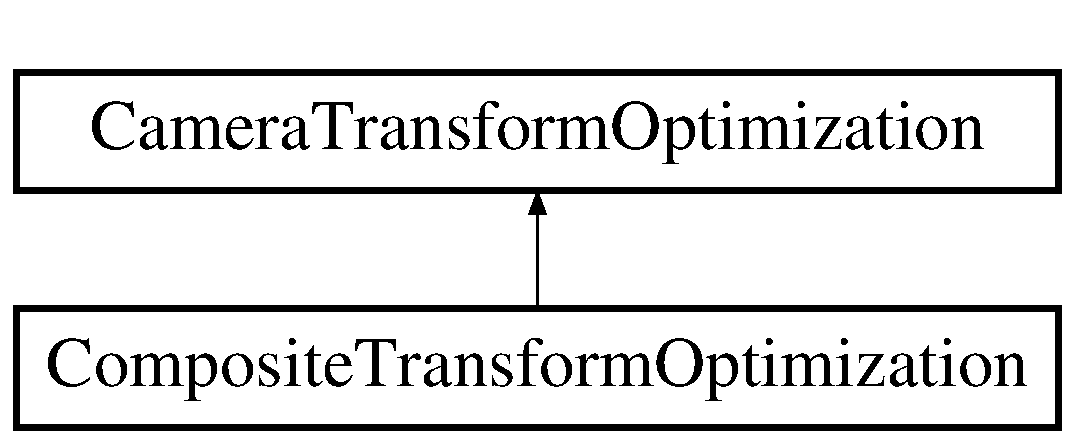
\includegraphics[height=2.000000cm]{classCompositeTransformOptimization}
\end{center}
\end{figure}
\subsection*{\-Public \-Member \-Functions}
\begin{DoxyCompactItemize}
\item 
\hypertarget{classCompositeTransformOptimization_a3a0ba4201758b8917059faf41f7f106b}{void {\bfseries add\-Transform\-Optimization} (std\-::string name, \hyperlink{classCameraTransformOptimization}{\-Camera\-Transform\-Optimization} $\ast$to)}\label{classCompositeTransformOptimization_a3a0ba4201758b8917059faf41f7f106b}

\item 
virtual void \hyperlink{classCompositeTransformOptimization_aa77358fb8292c767bfbf029115ced9cf}{optimize\-Transform} (\hyperlink{classCalibrationState}{\-Calibration\-State} \&calibration\-State)
\item 
virtual void \hyperlink{classCompositeTransformOptimization_aff2a0c0afce22998d1a1128b1671d99c}{add\-Measure\-Point} (\hyperlink{classCameraMeasurePoint}{\-Measure\-Point} new\-Point)
\item 
virtual void \hyperlink{classCompositeTransformOptimization_a5313f4fff02e5d48a7007af68ea6f008}{clear\-Measure\-Points} ()
\item 
\hypertarget{classCompositeTransformOptimization_ae6ba2a0afb45a340fb1919fe92e70156}{virtual void {\bfseries set\-Initial\-Camera\-To\-Head} (tf\-::\-Transform initial\-Transform)}\label{classCompositeTransformOptimization_ae6ba2a0afb45a340fb1919fe92e70156}

\end{DoxyCompactItemize}


\subsection{\-Detailed \-Description}
\-Container for multiple optimizers. 

\subsection{\-Member \-Function \-Documentation}
\hypertarget{classCompositeTransformOptimization_aff2a0c0afce22998d1a1128b1671d99c}{\index{\-Composite\-Transform\-Optimization@{\-Composite\-Transform\-Optimization}!add\-Measure\-Point@{add\-Measure\-Point}}
\index{add\-Measure\-Point@{add\-Measure\-Point}!CompositeTransformOptimization@{\-Composite\-Transform\-Optimization}}
\subsubsection[{add\-Measure\-Point}]{\setlength{\rightskip}{0pt plus 5cm}void {\bf \-Composite\-Transform\-Optimization\-::add\-Measure\-Point} (
\begin{DoxyParamCaption}
\item[{{\bf \-Measure\-Point}}]{new\-Point}
\end{DoxyParamCaption}
)\hspace{0.3cm}{\ttfamily  \mbox{[}virtual\mbox{]}}}}\label{classCompositeTransformOptimization_aff2a0c0afce22998d1a1128b1671d99c}
\-Adds a new measure point. 

\-Reimplemented from \hyperlink{classCameraTransformOptimization_ac1ffbf2ddfc7e7de7639e870d0745957}{\-Camera\-Transform\-Optimization}.

\hypertarget{classCompositeTransformOptimization_a5313f4fff02e5d48a7007af68ea6f008}{\index{\-Composite\-Transform\-Optimization@{\-Composite\-Transform\-Optimization}!clear\-Measure\-Points@{clear\-Measure\-Points}}
\index{clear\-Measure\-Points@{clear\-Measure\-Points}!CompositeTransformOptimization@{\-Composite\-Transform\-Optimization}}
\subsubsection[{clear\-Measure\-Points}]{\setlength{\rightskip}{0pt plus 5cm}void {\bf \-Composite\-Transform\-Optimization\-::clear\-Measure\-Points} (
\begin{DoxyParamCaption}
{}
\end{DoxyParamCaption}
)\hspace{0.3cm}{\ttfamily  \mbox{[}virtual\mbox{]}}}}\label{classCompositeTransformOptimization_a5313f4fff02e5d48a7007af68ea6f008}
\-Clears the list of measure points. 

\-Reimplemented from \hyperlink{classCameraTransformOptimization_a53007c5c531dd86a5facf7cbc82f477e}{\-Camera\-Transform\-Optimization}.

\hypertarget{classCompositeTransformOptimization_aa77358fb8292c767bfbf029115ced9cf}{\index{\-Composite\-Transform\-Optimization@{\-Composite\-Transform\-Optimization}!optimize\-Transform@{optimize\-Transform}}
\index{optimize\-Transform@{optimize\-Transform}!CompositeTransformOptimization@{\-Composite\-Transform\-Optimization}}
\subsubsection[{optimize\-Transform}]{\setlength{\rightskip}{0pt plus 5cm}void {\bf \-Composite\-Transform\-Optimization\-::optimize\-Transform} (
\begin{DoxyParamCaption}
\item[{{\bf \-Calibration\-State} \&}]{calibration\-State}
\end{DoxyParamCaption}
)\hspace{0.3cm}{\ttfamily  \mbox{[}virtual\mbox{]}}}}\label{classCompositeTransformOptimization_aa77358fb8292c767bfbf029115ced9cf}
\-Returns the best results with repsect to the error function. 

\-Implements \hyperlink{classCameraTransformOptimization_a8a4a4a09325f4bae401bad62ec7e9f02}{\-Camera\-Transform\-Optimization}.



\-The documentation for this class was generated from the following files\-:\begin{DoxyCompactItemize}
\item 
/home/stefan/catkin\-\_\-ws/src/calibration/include/\-Camera\-Transform\-Optimization.\-h\item 
/home/stefan/catkin\-\_\-ws/src/calibration/src/\-Camera\-Transform\-Optimization.\-cpp\end{DoxyCompactItemize}

\hypertarget{classDataCaptureParameter}{\section{\-Data\-Capture\-Parameter \-Class \-Reference}
\label{classDataCaptureParameter}\index{\-Data\-Capture\-Parameter@{\-Data\-Capture\-Parameter}}
}
\subsection*{\-Public \-Member \-Functions}
\begin{DoxyCompactItemize}
\item 
\hypertarget{classDataCaptureParameter_a4093e9c66b27849b450bf1bcab7ac35c}{int {\bfseries get\-Buffer\-Size} () const }\label{classDataCaptureParameter_a4093e9c66b27849b450bf1bcab7ac35c}

\item 
\hypertarget{classDataCaptureParameter_aacc7e04c950a9faeec620666eeab7ada}{void {\bfseries set\-Buffer\-Size} (int buffer\-Size)}\label{classDataCaptureParameter_aacc7e04c950a9faeec620666eeab7ada}

\item 
\hypertarget{classDataCaptureParameter_ae1a89313d8378d198adef62ea7b64ab9}{string {\bfseries get\-Camera\-Frame} () const }\label{classDataCaptureParameter_ae1a89313d8378d198adef62ea7b64ab9}

\item 
\hypertarget{classDataCaptureParameter_a7c99eb34bd0ee36ab27591ca465e9981}{void {\bfseries set\-Camera\-Frame} (string camera\-Frame)}\label{classDataCaptureParameter_a7c99eb34bd0ee36ab27591ca465e9981}

\item 
\hypertarget{classDataCaptureParameter_ab68428f31daf6f9e4a537cc3144cdc61}{string {\bfseries get\-Fixed\-Frame} () const }\label{classDataCaptureParameter_ab68428f31daf6f9e4a537cc3144cdc61}

\item 
\hypertarget{classDataCaptureParameter_a7132c6affa2fe957772d9723080e8349}{void {\bfseries set\-Fixed\-Frame} (string fixed\-Frame)}\label{classDataCaptureParameter_a7132c6affa2fe957772d9723080e8349}

\item 
\hypertarget{classDataCaptureParameter_a9ea7189cf620f5ce6ce986151ae59678}{string {\bfseries get\-Footprint\-Frame} () const }\label{classDataCaptureParameter_a9ea7189cf620f5ce6ce986151ae59678}

\item 
\hypertarget{classDataCaptureParameter_a4435144260e57fdba3bc43ff34d5fd4e}{void {\bfseries set\-Footprint\-Frame} (string footprint\-Frame)}\label{classDataCaptureParameter_a4435144260e57fdba3bc43ff34d5fd4e}

\item 
\hypertarget{classDataCaptureParameter_a5a656f09e189765f4707f0291a04d107}{string {\bfseries get\-Head\-Pitch\-Frame} () const }\label{classDataCaptureParameter_a5a656f09e189765f4707f0291a04d107}

\item 
\hypertarget{classDataCaptureParameter_a01a144de3e8c49392a49ea0e4d846ba2}{void {\bfseries set\-Head\-Pitch\-Frame} (string head\-Pitch\-Frame)}\label{classDataCaptureParameter_a01a144de3e8c49392a49ea0e4d846ba2}

\item 
\hypertarget{classDataCaptureParameter_a8a1f406cb9c9bc3b097c648141a082cf}{string {\bfseries get\-Head\-Yaw\-Frame} () const }\label{classDataCaptureParameter_a8a1f406cb9c9bc3b097c648141a082cf}

\item 
\hypertarget{classDataCaptureParameter_a000c6bb2bba31a030425eed7c01f9751}{void {\bfseries set\-Head\-Yaw\-Frame} (string head\-Yaw\-Frame)}\label{classDataCaptureParameter_a000c6bb2bba31a030425eed7c01f9751}

\item 
\hypertarget{classDataCaptureParameter_aafba952669f9b6e29df5db6e20caab52}{int {\bfseries get\-Min\-Num\-Of\-Measurements} () const }\label{classDataCaptureParameter_aafba952669f9b6e29df5db6e20caab52}

\item 
\hypertarget{classDataCaptureParameter_a429177cbbff516470ded32526c90e9ed}{void {\bfseries set\-Min\-Num\-Of\-Measurements} (int min\-Num\-Of\-Measurements)}\label{classDataCaptureParameter_a429177cbbff516470ded32526c90e9ed}

\item 
\hypertarget{classDataCaptureParameter_a6c2c713fced1812014cfd99ec8713813}{string {\bfseries get\-Optical\-Frame} () const }\label{classDataCaptureParameter_a6c2c713fced1812014cfd99ec8713813}

\item 
\hypertarget{classDataCaptureParameter_a5e36293ddcd307146015f01d4800f8ce}{void {\bfseries set\-Optical\-Frame} (string optical\-Frame)}\label{classDataCaptureParameter_a5e36293ddcd307146015f01d4800f8ce}

\item 
\hypertarget{classDataCaptureParameter_a4f06c9d1aadc46c1200200ef7e278d54}{string {\bfseries get\-Point\-Cloud\-Topic} () const }\label{classDataCaptureParameter_a4f06c9d1aadc46c1200200ef7e278d54}

\item 
\hypertarget{classDataCaptureParameter_a6e09fccfe4dfdde6965ad42357feb109}{void {\bfseries set\-Point\-Cloud\-Topic} (string point\-Cloud\-Topic)}\label{classDataCaptureParameter_a6e09fccfe4dfdde6965ad42357feb109}

\item 
\hypertarget{classDataCaptureParameter_a6cdf52ecd14fadc17154d2ae5dcdc9d4}{string {\bfseries get\-Torso\-Frame} () const }\label{classDataCaptureParameter_a6cdf52ecd14fadc17154d2ae5dcdc9d4}

\item 
\hypertarget{classDataCaptureParameter_a540d67f30f2ee09656ecca826c463ab6}{void {\bfseries set\-Torso\-Frame} (string torso\-Frame)}\label{classDataCaptureParameter_a540d67f30f2ee09656ecca826c463ab6}

\end{DoxyCompactItemize}
\subsection*{\-Protected \-Attributes}
\begin{DoxyCompactItemize}
\item 
\hypertarget{classDataCaptureParameter_ad1d2d774a86554b5432a426a9f46f58d}{string {\bfseries point\-Cloud\-Topic}}\label{classDataCaptureParameter_ad1d2d774a86554b5432a426a9f46f58d}

\item 
\hypertarget{classDataCaptureParameter_a0d5780e5728d747a3affb4c3a8df9123}{string {\bfseries optical\-Frame}}\label{classDataCaptureParameter_a0d5780e5728d747a3affb4c3a8df9123}

\item 
\hypertarget{classDataCaptureParameter_ab36fbe41e45a5a9ed228ea7b9c2a890a}{string {\bfseries camera\-Frame}}\label{classDataCaptureParameter_ab36fbe41e45a5a9ed228ea7b9c2a890a}

\item 
\hypertarget{classDataCaptureParameter_abec1f13f13e852fa19c10adb22f13103}{string {\bfseries head\-Pitch\-Frame}}\label{classDataCaptureParameter_abec1f13f13e852fa19c10adb22f13103}

\item 
\hypertarget{classDataCaptureParameter_abd148eef2a26c380adba80118e7cf377}{string {\bfseries head\-Yaw\-Frame}}\label{classDataCaptureParameter_abd148eef2a26c380adba80118e7cf377}

\item 
\hypertarget{classDataCaptureParameter_a71aa2555bb4a64e4e7fc69a5a9793cf5}{string {\bfseries torso\-Frame}}\label{classDataCaptureParameter_a71aa2555bb4a64e4e7fc69a5a9793cf5}

\item 
\hypertarget{classDataCaptureParameter_a0685528cb6df9b9474d15b931fefb26f}{string {\bfseries fixed\-Frame}}\label{classDataCaptureParameter_a0685528cb6df9b9474d15b931fefb26f}

\item 
\hypertarget{classDataCaptureParameter_ae5e91334057f59d9ad720d83a69d3f2b}{string {\bfseries footprint\-Frame}}\label{classDataCaptureParameter_ae5e91334057f59d9ad720d83a69d3f2b}

\item 
\hypertarget{classDataCaptureParameter_a93d1c583c29328029848a02621a16331}{int {\bfseries min\-Num\-Of\-Measurements}}\label{classDataCaptureParameter_a93d1c583c29328029848a02621a16331}

\item 
\hypertarget{classDataCaptureParameter_aa38b11eae67d098431f389f2eeb8ff73}{int {\bfseries buffer\-Size}}\label{classDataCaptureParameter_aa38b11eae67d098431f389f2eeb8ff73}

\end{DoxyCompactItemize}


\-The documentation for this class was generated from the following file\-:\begin{DoxyCompactItemize}
\item 
/home/stefan/catkin\-\_\-ws/src/calibration/include/\-Parameter.\-h\end{DoxyCompactItemize}

\hypertarget{classEdgeGroundMeasurement}{\section{\-Edge\-Ground\-Measurement \-Class \-Reference}
\label{classEdgeGroundMeasurement}\index{\-Edge\-Ground\-Measurement@{\-Edge\-Ground\-Measurement}}
}
\subsection*{\-Public \-Member \-Functions}
\begin{DoxyCompactItemize}
\item 
\hypertarget{classEdgeGroundMeasurement_ae00976acc5f489fe8568a8233fbc1272}{{\bfseries \-Edge\-Ground\-Measurement} (\hyperlink{classCameraMeasurePoint}{\-Measure\-Point} \&measure\-Point, double ground\-Distance)}\label{classEdgeGroundMeasurement_ae00976acc5f489fe8568a8233fbc1272}

\item 
\hypertarget{classEdgeGroundMeasurement_af75822a92c61e0adb9331b2ec55d958a}{virtual void {\bfseries compute\-Error} ()}\label{classEdgeGroundMeasurement_af75822a92c61e0adb9331b2ec55d958a}

\item 
\hypertarget{classEdgeGroundMeasurement_a87de21dbfa80bc1488efd1de22457b5e}{virtual bool {\bfseries read} (std\-::istream \&is)}\label{classEdgeGroundMeasurement_a87de21dbfa80bc1488efd1de22457b5e}

\item 
\hypertarget{classEdgeGroundMeasurement_af94851587e2ce97f359f4b9819c56645}{virtual bool {\bfseries write} (std\-::ostream \&os) const }\label{classEdgeGroundMeasurement_af94851587e2ce97f359f4b9819c56645}

\end{DoxyCompactItemize}
\subsection*{\-Protected \-Attributes}
\begin{DoxyCompactItemize}
\item 
\hypertarget{classEdgeGroundMeasurement_a904e8c85e72111cc476149263e161c08}{\hyperlink{classCameraMeasurePoint}{\-Measure\-Point} \& {\bfseries measure\-Point}}\label{classEdgeGroundMeasurement_a904e8c85e72111cc476149263e161c08}

\item 
\hypertarget{classEdgeGroundMeasurement_a3ab164b8559ee9e5f4c503b620866bd3}{double {\bfseries ground\-Distance}}\label{classEdgeGroundMeasurement_a3ab164b8559ee9e5f4c503b620866bd3}

\end{DoxyCompactItemize}


\-The documentation for this class was generated from the following files\-:\begin{DoxyCompactItemize}
\item 
/home/stefan/catkin\-\_\-ws/src/calibration/include/\-Edge\-Ground\-Measurement.\-h\item 
/home/stefan/catkin\-\_\-ws/src/calibration/src/\-Edge\-Ground\-Measurement.\-cpp\end{DoxyCompactItemize}

\hypertarget{classEdgeMarkerMeasurement}{\section{\-Edge\-Marker\-Measurement \-Class \-Reference}
\label{classEdgeMarkerMeasurement}\index{\-Edge\-Marker\-Measurement@{\-Edge\-Marker\-Measurement}}
}
\subsection*{\-Public \-Member \-Functions}
\begin{DoxyCompactItemize}
\item 
\hypertarget{classEdgeMarkerMeasurement_a66b96b376f59572a10bf25ea45989418}{{\bfseries \-Edge\-Marker\-Measurement} (\hyperlink{classCameraMeasurePoint}{\-Measure\-Point} \&measure\-Point, \hyperlink{classMarkerEstimation}{\-Marker\-Estimation} \&marker\-Estimation)}\label{classEdgeMarkerMeasurement_a66b96b376f59572a10bf25ea45989418}

\item 
\hypertarget{classEdgeMarkerMeasurement_af57e5dcfd6f1742990420364163dbc52}{virtual void {\bfseries compute\-Error} ()}\label{classEdgeMarkerMeasurement_af57e5dcfd6f1742990420364163dbc52}

\item 
\hypertarget{classEdgeMarkerMeasurement_a95396b4d4b56fb4d108de6c36acdf57a}{virtual bool {\bfseries read} (std\-::istream \&is)}\label{classEdgeMarkerMeasurement_a95396b4d4b56fb4d108de6c36acdf57a}

\item 
\hypertarget{classEdgeMarkerMeasurement_a9027128d76b86004d3fb2fc065328cf1}{virtual bool {\bfseries write} (std\-::ostream \&os) const }\label{classEdgeMarkerMeasurement_a9027128d76b86004d3fb2fc065328cf1}

\end{DoxyCompactItemize}
\subsection*{\-Protected \-Attributes}
\begin{DoxyCompactItemize}
\item 
\hypertarget{classEdgeMarkerMeasurement_a04b8a29d135d3c5687e195fc27785575}{\hyperlink{classCameraMeasurePoint}{\-Measure\-Point} \& {\bfseries measure\-Point}}\label{classEdgeMarkerMeasurement_a04b8a29d135d3c5687e195fc27785575}

\item 
\hypertarget{classEdgeMarkerMeasurement_a4f8c0a995405bac1af1bc7f47db23a50}{\hyperlink{classMarkerEstimation}{\-Marker\-Estimation} \& {\bfseries marker\-Estimation}}\label{classEdgeMarkerMeasurement_a4f8c0a995405bac1af1bc7f47db23a50}

\end{DoxyCompactItemize}


\-The documentation for this class was generated from the following files\-:\begin{DoxyCompactItemize}
\item 
/home/stefan/catkin\-\_\-ws/src/calibration/include/\-Edge\-Marker\-Measurement.\-h\item 
/home/stefan/catkin\-\_\-ws/src/calibration/src/\-Edge\-Marker\-Measurement.\-cpp\end{DoxyCompactItemize}

\hypertarget{classG2oTransformOptimization}{\section{\-G2o\-Transform\-Optimization \-Class \-Reference}
\label{classG2oTransformOptimization}\index{\-G2o\-Transform\-Optimization@{\-G2o\-Transform\-Optimization}}
}
\-Inheritance diagram for \-G2o\-Transform\-Optimization\-:\begin{figure}[H]
\begin{center}
\leavevmode
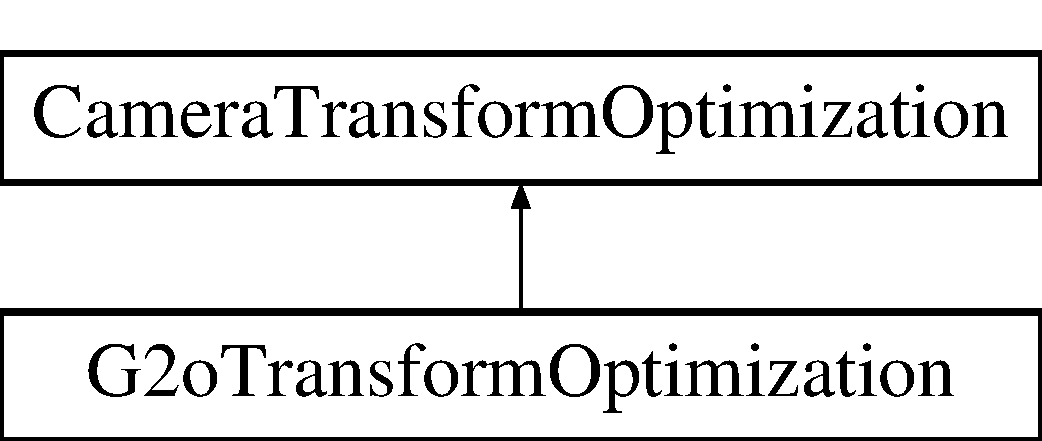
\includegraphics[height=2.000000cm]{classG2oTransformOptimization}
\end{center}
\end{figure}
\subsection*{\-Public \-Member \-Functions}
\begin{DoxyCompactItemize}
\item 
\hypertarget{classG2oTransformOptimization_a41c3b47772cfaa74e0d6a6dbaa853d11}{{\bfseries \-G2o\-Transform\-Optimization} (\hyperlink{classCameraTransformOptimizationParameter}{\-Camera\-Transform\-Optimization\-Parameter} parameter=\hyperlink{classCameraTransformOptimizationParameter}{\-Camera\-Transform\-Optimization\-Parameter}())}\label{classG2oTransformOptimization_a41c3b47772cfaa74e0d6a6dbaa853d11}

\item 
virtual void \hyperlink{classG2oTransformOptimization_a8a644d4ab3d5cacd4cc56f716dfd648d}{optimize\-Transform} (\hyperlink{classCalibrationState}{\-Calibration\-State} \&calibration\-State)
\item 
virtual void \hyperlink{classG2oTransformOptimization_a2b3606f70377e7736712c131fe48d1ae}{get\-Marker\-Estimate} (const \hyperlink{classCalibrationState}{\-Calibration\-State} \&state, tf\-::\-Vector3 \&position)
\item 
\hypertarget{classG2oTransformOptimization_a4d661d25a7b57ebf389d5fb9e22d7e27}{\-Eigen\-::\-Matrix$<$ double, 5, 5 $>$ {\bfseries get\-Correlation\-Matrix} () const }\label{classG2oTransformOptimization_a4d661d25a7b57ebf389d5fb9e22d7e27}

\item 
\hypertarget{classG2oTransformOptimization_a2e926b516a5b1b3a81b395f986c86bbc}{void {\bfseries set\-Correlation\-Matrix} (\-Eigen\-::\-Matrix$<$ double, 5, 5 $>$ correlation\-Matrix)}\label{classG2oTransformOptimization_a2e926b516a5b1b3a81b395f986c86bbc}

\end{DoxyCompactItemize}


\subsection{\-Member \-Function \-Documentation}
\hypertarget{classG2oTransformOptimization_a2b3606f70377e7736712c131fe48d1ae}{\index{\-G2o\-Transform\-Optimization@{\-G2o\-Transform\-Optimization}!get\-Marker\-Estimate@{get\-Marker\-Estimate}}
\index{get\-Marker\-Estimate@{get\-Marker\-Estimate}!G2oTransformOptimization@{\-G2o\-Transform\-Optimization}}
\subsubsection[{get\-Marker\-Estimate}]{\setlength{\rightskip}{0pt plus 5cm}void {\bf \-G2o\-Transform\-Optimization\-::get\-Marker\-Estimate} (
\begin{DoxyParamCaption}
\item[{const {\bf \-Calibration\-State} \&}]{camera\-To\-Head, }
\item[{tf\-::\-Vector3 \&}]{position}
\end{DoxyParamCaption}
)\hspace{0.3cm}{\ttfamily  \mbox{[}virtual\mbox{]}}}}\label{classG2oTransformOptimization_a2b3606f70377e7736712c131fe48d1ae}
\-Calculates an estimate for the marker position given a guess for the transformation. 

\-Reimplemented from \hyperlink{classCameraTransformOptimization_a63da0977758e7a4b63f946ada33e7dd5}{\-Camera\-Transform\-Optimization}.

\hypertarget{classG2oTransformOptimization_a8a644d4ab3d5cacd4cc56f716dfd648d}{\index{\-G2o\-Transform\-Optimization@{\-G2o\-Transform\-Optimization}!optimize\-Transform@{optimize\-Transform}}
\index{optimize\-Transform@{optimize\-Transform}!G2oTransformOptimization@{\-G2o\-Transform\-Optimization}}
\subsubsection[{optimize\-Transform}]{\setlength{\rightskip}{0pt plus 5cm}void {\bf \-G2o\-Transform\-Optimization\-::optimize\-Transform} (
\begin{DoxyParamCaption}
\item[{{\bf \-Calibration\-State} \&}]{calibration\-State}
\end{DoxyParamCaption}
)\hspace{0.3cm}{\ttfamily  \mbox{[}virtual\mbox{]}}}}\label{classG2oTransformOptimization_a8a644d4ab3d5cacd4cc56f716dfd648d}
\-Optimizes the transform given the measured points, initial transformation, and all other transformations needed. 

\-Implements \hyperlink{classCameraTransformOptimization_a8a4a4a09325f4bae401bad62ec7e9f02}{\-Camera\-Transform\-Optimization}.



\-The documentation for this class was generated from the following files\-:\begin{DoxyCompactItemize}
\item 
/home/stefan/catkin\-\_\-ws/src/calibration/include/\-G2o\-Transform\-Optimization.\-h\item 
/home/stefan/catkin\-\_\-ws/src/calibration/src/\-G2o\-Transform\-Optimization.\-cpp\end{DoxyCompactItemize}

\hypertarget{classGroundData}{\section{\-Ground\-Data \-Class \-Reference}
\label{classGroundData}\index{\-Ground\-Data@{\-Ground\-Data}}
}
\subsection*{\-Public \-Member \-Functions}
\begin{DoxyCompactItemize}
\item 
\hypertarget{classGroundData_aa29b6ae9004fb510f3a1262337fa3bad}{tf\-::\-Pose {\bfseries get\-Pose} () const }\label{classGroundData_aa29b6ae9004fb510f3a1262337fa3bad}

\item 
\hypertarget{classGroundData_af31ca9c984769df196ca32332d960f1e}{void {\bfseries get\-R\-P\-Y} (double \&roll, double \&pitch, double \&yaw) const }\label{classGroundData_af31ca9c984769df196ca32332d960f1e}

\item 
\hypertarget{classGroundData_ae25ff85d1fa8f88ec8e8a7e5bf1774da}{void {\bfseries set\-Equation} (float a, float b, float c, float d)}\label{classGroundData_ae25ff85d1fa8f88ec8e8a7e5bf1774da}

\item 
\hypertarget{classGroundData_a4299c07208ef50609639f0c9bd8d1a8a}{\hyperlink{classGroundData}{\-Ground\-Data} {\bfseries transform} (tf\-::\-Transform) const }\label{classGroundData_a4299c07208ef50609639f0c9bd8d1a8a}

\end{DoxyCompactItemize}
\subsection*{\-Static \-Public \-Member \-Functions}
\begin{DoxyCompactItemize}
\item 
\hypertarget{classGroundData_a9964261c8d5cfd05c7ae7a18150f9c00}{static double {\bfseries normalize} (double angle)}\label{classGroundData_a9964261c8d5cfd05c7ae7a18150f9c00}

\end{DoxyCompactItemize}
\subsection*{\-Public \-Attributes}
\begin{DoxyCompactItemize}
\item 
\hypertarget{classGroundData_a1fb86e0af3b29fe06e944a409ac01151}{double {\bfseries a}}\label{classGroundData_a1fb86e0af3b29fe06e944a409ac01151}

\item 
\hypertarget{classGroundData_a2cdcf741a7a0bcb2d7b2ef1eb3aa83c6}{double {\bfseries b}}\label{classGroundData_a2cdcf741a7a0bcb2d7b2ef1eb3aa83c6}

\item 
\hypertarget{classGroundData_a3ec92519e2c1e34f503e41a00a0da5e1}{double {\bfseries c}}\label{classGroundData_a3ec92519e2c1e34f503e41a00a0da5e1}

\item 
\hypertarget{classGroundData_a1272c9dc45835fa2e260e28fdfd585b5}{double {\bfseries d}}\label{classGroundData_a1272c9dc45835fa2e260e28fdfd585b5}

\end{DoxyCompactItemize}
\subsection*{\-Protected \-Member \-Functions}
\begin{DoxyCompactItemize}
\item 
\hypertarget{classGroundData_a3abf6b3d83c832202aabb1aabc58b877}{void {\bfseries calculate\-Points\-From\-Equation} ()}\label{classGroundData_a3abf6b3d83c832202aabb1aabc58b877}

\item 
\hypertarget{classGroundData_a80b35f02d5a93dbcb6e13c9fd1116f8e}{void {\bfseries calculate\-Equation\-From\-Points} ()}\label{classGroundData_a80b35f02d5a93dbcb6e13c9fd1116f8e}

\item 
\hypertarget{classGroundData_afc48a5e845ef99030e6fd4b2e67dc5e7}{void {\bfseries normalize\-Equation} ()}\label{classGroundData_afc48a5e845ef99030e6fd4b2e67dc5e7}

\end{DoxyCompactItemize}
\subsection*{\-Protected \-Attributes}
\begin{DoxyCompactItemize}
\item 
\hypertarget{classGroundData_a7f01fcceb40d9fe1e90b9707a0f27d12}{tf\-::\-Vector3 {\bfseries point\-One}}\label{classGroundData_a7f01fcceb40d9fe1e90b9707a0f27d12}

\item 
\hypertarget{classGroundData_a9eb9983429699256738d73cf3c0a7966}{tf\-::\-Vector3 {\bfseries point\-Two}}\label{classGroundData_a9eb9983429699256738d73cf3c0a7966}

\item 
\hypertarget{classGroundData_aa7b6a40d7d2fb99a93eb62b9929b6684}{tf\-::\-Vector3 {\bfseries point\-Three}}\label{classGroundData_aa7b6a40d7d2fb99a93eb62b9929b6684}

\end{DoxyCompactItemize}
\subsection*{\-Friends}
\begin{DoxyCompactItemize}
\item 
\hypertarget{classGroundData_aa4a16a3561c64b16b9c9b696af4546f7}{ostream \& {\bfseries operator$<$$<$} (ostream \&output, const \hyperlink{classGroundData}{\-Ground\-Data} \&gd)}\label{classGroundData_aa4a16a3561c64b16b9c9b696af4546f7}

\item 
\hypertarget{classGroundData_a7f52aaea73e092112650755b2c5041da}{istream \& {\bfseries operator$>$$>$} (istream \&input, \hyperlink{classGroundData}{\-Ground\-Data} \&gd)}\label{classGroundData_a7f52aaea73e092112650755b2c5041da}

\end{DoxyCompactItemize}


\-The documentation for this class was generated from the following files\-:\begin{DoxyCompactItemize}
\item 
/home/stefan/catkin\-\_\-ws/src/calibration/include/\-Ground\-Detection.\-h\item 
/home/stefan/catkin\-\_\-ws/src/calibration/src/\-Ground\-Detection.\-cpp\end{DoxyCompactItemize}

\hypertarget{classGroundDetection}{\section{\-Ground\-Detection \-Class \-Reference}
\label{classGroundDetection}\index{\-Ground\-Detection@{\-Ground\-Detection}}
}
\subsection*{\-Public \-Member \-Functions}
\begin{DoxyCompactItemize}
\item 
\hypertarget{classGroundDetection_aa991673a7cfb56095d072e736ebcfb7a}{\hyperlink{classGroundData}{\-Ground\-Data} {\bfseries get\-Ground\-Data} (pcl\-::\-Point\-Cloud$<$ pcl\-::\-Point\-X\-Y\-Z\-R\-G\-B $>$\-::\-Ptr initial\-Cloud)}\label{classGroundDetection_aa991673a7cfb56095d072e736ebcfb7a}

\end{DoxyCompactItemize}
\subsection*{\-Protected \-Member \-Functions}
\begin{DoxyCompactItemize}
\item 
\hypertarget{classGroundDetection_a252f44f0381a8f8acdfdd56e477cbfb7}{void {\bfseries filter\-Range} (pcl\-::\-Point\-Cloud$<$ pcl\-::\-Point\-X\-Y\-Z\-R\-G\-B $>$\-::\-Ptr in\-Cloud, pcl\-::\-Point\-Cloud$<$ pcl\-::\-Point\-X\-Y\-Z\-R\-G\-B $>$\-::\-Ptr out\-Cloud)}\label{classGroundDetection_a252f44f0381a8f8acdfdd56e477cbfb7}

\item 
\hypertarget{classGroundDetection_a13890fa639de4c021ca80121cffb76e3}{void {\bfseries segment\-Plane} (pcl\-::\-Point\-Cloud$<$ pcl\-::\-Point\-X\-Y\-Z\-R\-G\-B $>$\-::\-Ptr in\-Cloud, \hyperlink{classGroundData}{\-Ground\-Data} \&gd)}\label{classGroundDetection_a13890fa639de4c021ca80121cffb76e3}

\end{DoxyCompactItemize}


\-The documentation for this class was generated from the following files\-:\begin{DoxyCompactItemize}
\item 
/home/stefan/catkin\-\_\-ws/src/calibration/include/\-Ground\-Detection.\-h\item 
/home/stefan/catkin\-\_\-ws/src/calibration/src/\-Ground\-Detection.\-cpp\end{DoxyCompactItemize}

\hypertarget{classHillClimbingTransformOptimization}{\section{\-Hill\-Climbing\-Transform\-Optimization \-Class \-Reference}
\label{classHillClimbingTransformOptimization}\index{\-Hill\-Climbing\-Transform\-Optimization@{\-Hill\-Climbing\-Transform\-Optimization}}
}
\-Inheritance diagram for \-Hill\-Climbing\-Transform\-Optimization\-:\begin{figure}[H]
\begin{center}
\leavevmode
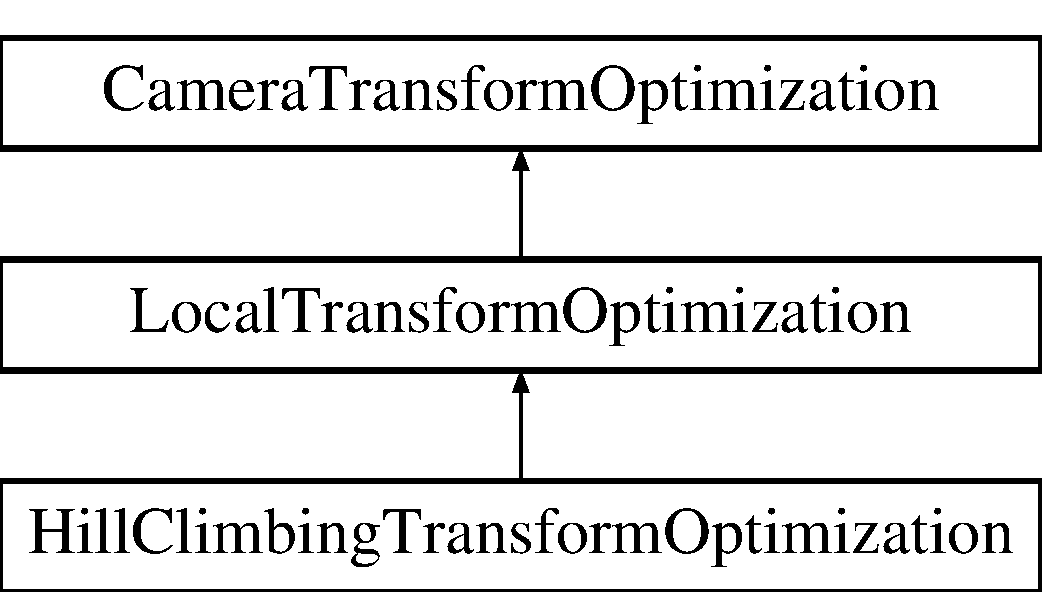
\includegraphics[height=3.000000cm]{classHillClimbingTransformOptimization}
\end{center}
\end{figure}
\subsection*{\-Public \-Member \-Functions}
\begin{DoxyCompactItemize}
\item 
\hypertarget{classHillClimbingTransformOptimization_aec6c9d518076d7a45fd084b4083b26ee}{{\bfseries \-Hill\-Climbing\-Transform\-Optimization} (\hyperlink{classCameraTransformOptimizationParameter}{\-Camera\-Transform\-Optimization\-Parameter} parameter=\hyperlink{classCameraTransformOptimizationParameter}{\-Camera\-Transform\-Optimization\-Parameter}())}\label{classHillClimbingTransformOptimization_aec6c9d518076d7a45fd084b4083b26ee}

\item 
virtual void \hyperlink{classHillClimbingTransformOptimization_a4f7fb583e57929790420e1f28d97c383}{optimize\-Transform} (\hyperlink{classCalibrationState}{\-Calibration\-State} \&calibration\-State)
\end{DoxyCompactItemize}


\subsection{\-Member \-Function \-Documentation}
\hypertarget{classHillClimbingTransformOptimization_a4f7fb583e57929790420e1f28d97c383}{\index{\-Hill\-Climbing\-Transform\-Optimization@{\-Hill\-Climbing\-Transform\-Optimization}!optimize\-Transform@{optimize\-Transform}}
\index{optimize\-Transform@{optimize\-Transform}!HillClimbingTransformOptimization@{\-Hill\-Climbing\-Transform\-Optimization}}
\subsubsection[{optimize\-Transform}]{\setlength{\rightskip}{0pt plus 5cm}void {\bf \-Hill\-Climbing\-Transform\-Optimization\-::optimize\-Transform} (
\begin{DoxyParamCaption}
\item[{{\bf \-Calibration\-State} \&}]{calibration\-State}
\end{DoxyParamCaption}
)\hspace{0.3cm}{\ttfamily  \mbox{[}virtual\mbox{]}}}}\label{classHillClimbingTransformOptimization_a4f7fb583e57929790420e1f28d97c383}
\-Optimizes the transform given the measured points, initial transformation, and all other transformations needed. 

\-Implements \hyperlink{classCameraTransformOptimization_a8a4a4a09325f4bae401bad62ec7e9f02}{\-Camera\-Transform\-Optimization}.



\-The documentation for this class was generated from the following files\-:\begin{DoxyCompactItemize}
\item 
/home/stefan/catkin\-\_\-ws/src/calibration/include/\-Local\-Transform\-Optimization.\-h\item 
/home/stefan/catkin\-\_\-ws/src/calibration/src/\-Local\-Transform\-Optimization.\-cpp\end{DoxyCompactItemize}

\hypertarget{classJointOffset}{\section{\-Joint\-Offset \-Class \-Reference}
\label{classJointOffset}\index{\-Joint\-Offset@{\-Joint\-Offset}}
}
\subsection*{\-Public \-Member \-Functions}
\begin{DoxyCompactItemize}
\item 
\hypertarget{classJointOffset_a1f9d93ce12e8c3598a3925da7ed0bc65}{void {\bfseries get\-Transformation} (string from, string to, double offset)}\label{classJointOffset_a1f9d93ce12e8c3598a3925da7ed0bc65}

\item 
\hypertarget{classJointOffset_af0a5608b9766a8ff4c26d4625358d727}{void {\bfseries initialize\-From\-Ros} ()}\label{classJointOffset_af0a5608b9766a8ff4c26d4625358d727}

\item 
\hypertarget{classJointOffset_a967bb552c3d01de5f296dff47291ea69}{void {\bfseries initialize\-From\-Urdf} (string urdf\-Xml)}\label{classJointOffset_a967bb552c3d01de5f296dff47291ea69}

\end{DoxyCompactItemize}
\subsection*{\-Protected \-Member \-Functions}
\begin{DoxyCompactItemize}
\item 
\hypertarget{classJointOffset_a24ece39d95a5fac5be88fc2691d82a16}{bool {\bfseries load\-Urdf\-From\-Ros} ()}\label{classJointOffset_a24ece39d95a5fac5be88fc2691d82a16}

\item 
\hypertarget{classJointOffset_a985a24ef7973b8378b5e4c226ac7cd64}{bool {\bfseries load\-Kdl\-From\-Urdf} ()}\label{classJointOffset_a985a24ef7973b8378b5e4c226ac7cd64}

\item 
\hypertarget{classJointOffset_a3e7e5bc603ba006e0250af9098186a91}{bool {\bfseries urdf\-String\-To\-Model} ()}\label{classJointOffset_a3e7e5bc603ba006e0250af9098186a91}

\item 
\hypertarget{classJointOffset_aceb352a0fb3c8335ff69f742d76bba82}{void {\bfseries add\-Children} (const \-K\-D\-L\-::\-Segment\-Map\-::const\-\_\-iterator segment)}\label{classJointOffset_aceb352a0fb3c8335ff69f742d76bba82}

\end{DoxyCompactItemize}


\-The documentation for this class was generated from the following files\-:\begin{DoxyCompactItemize}
\item 
/home/stefan/catkin\-\_\-ws/src/calibration/src/\-Joint\-Offset.\-h\item 
/home/stefan/catkin\-\_\-ws/src/calibration/include/\-Joint\-Offset.\-cpp\end{DoxyCompactItemize}

\hypertarget{classLocalTransformOptimization}{\section{\-Local\-Transform\-Optimization \-Class \-Reference}
\label{classLocalTransformOptimization}\index{\-Local\-Transform\-Optimization@{\-Local\-Transform\-Optimization}}
}
\-Inheritance diagram for \-Local\-Transform\-Optimization\-:\begin{figure}[H]
\begin{center}
\leavevmode
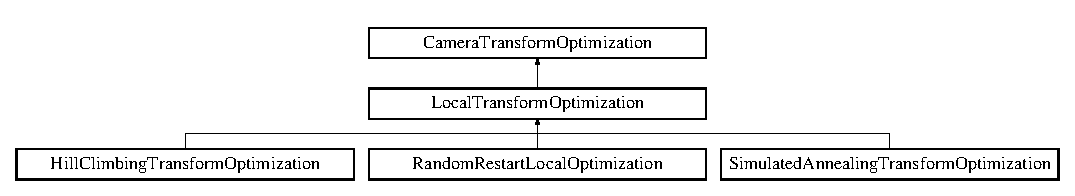
\includegraphics[height=2.187500cm]{classLocalTransformOptimization}
\end{center}
\end{figure}
\subsection*{\-Public \-Member \-Functions}
\begin{DoxyCompactItemize}
\item 
\hypertarget{classLocalTransformOptimization_ab4017ab5dead7c68ae6bacd9aeceeb59}{{\bfseries \-Local\-Transform\-Optimization} (\hyperlink{classCameraTransformOptimizationParameter}{\-Camera\-Transform\-Optimization\-Parameter} parameter=\hyperlink{classCameraTransformOptimizationParameter}{\-Camera\-Transform\-Optimization\-Parameter}())}\label{classLocalTransformOptimization_ab4017ab5dead7c68ae6bacd9aeceeb59}

\item 
\hypertarget{classLocalTransformOptimization_a86d6149a04bb57a901a3ce2ffe545eea}{virtual void {\bfseries set\-Initial\-State} (\hyperlink{classLtoState}{\-Lto\-State} initial\-State)}\label{classLocalTransformOptimization_a86d6149a04bb57a901a3ce2ffe545eea}

\end{DoxyCompactItemize}
\subsection*{\-Protected \-Member \-Functions}
\begin{DoxyCompactItemize}
\item 
\hypertarget{classLocalTransformOptimization_a2bb7c73654687e884b77854eaad0d94a}{bool {\bfseries decrease\-Stepwidth} ()}\label{classLocalTransformOptimization_a2bb7c73654687e884b77854eaad0d94a}

\item 
\hypertarget{classLocalTransformOptimization_a0c7eb89f2b531e5d618fdbea186d9663}{float {\bfseries calculate\-Error} (\hyperlink{classLtoState}{\-Lto\-State} \&other)}\label{classLocalTransformOptimization_a0c7eb89f2b531e5d618fdbea186d9663}

\item 
\hypertarget{classLocalTransformOptimization_a39cf1ac8cbb3db7d5c8ee2194788b4cc}{virtual std\-::vector$<$ \hyperlink{classLtoState}{\-Lto\-State} $>$ {\bfseries get\-Neighbors} (\hyperlink{classLtoState}{\-Lto\-State} \&current)}\label{classLocalTransformOptimization_a39cf1ac8cbb3db7d5c8ee2194788b4cc}

\end{DoxyCompactItemize}
\subsection*{\-Protected \-Attributes}
\begin{DoxyCompactItemize}
\item 
\hypertarget{classLocalTransformOptimization_a77ed4f8e7e3439eccd1fedbd643a27a9}{float {\bfseries stepwidth}}\label{classLocalTransformOptimization_a77ed4f8e7e3439eccd1fedbd643a27a9}

\item 
\hypertarget{classLocalTransformOptimization_a8d7a4401a591d3274d107e32b1a524e3}{\hyperlink{classLtoState}{\-Lto\-State} {\bfseries initial\-State}}\label{classLocalTransformOptimization_a8d7a4401a591d3274d107e32b1a524e3}

\end{DoxyCompactItemize}


\-The documentation for this class was generated from the following files\-:\begin{DoxyCompactItemize}
\item 
/home/stefan/catkin\-\_\-ws/src/calibration/include/\-Local\-Transform\-Optimization.\-h\item 
/home/stefan/catkin\-\_\-ws/src/calibration/src/\-Local\-Transform\-Optimization.\-cpp\end{DoxyCompactItemize}

\hypertarget{classLtoState}{\section{\-Lto\-State \-Class \-Reference}
\label{classLtoState}\index{\-Lto\-State@{\-Lto\-State}}
}
\-Inheritance diagram for \-Lto\-State\-:\begin{figure}[H]
\begin{center}
\leavevmode
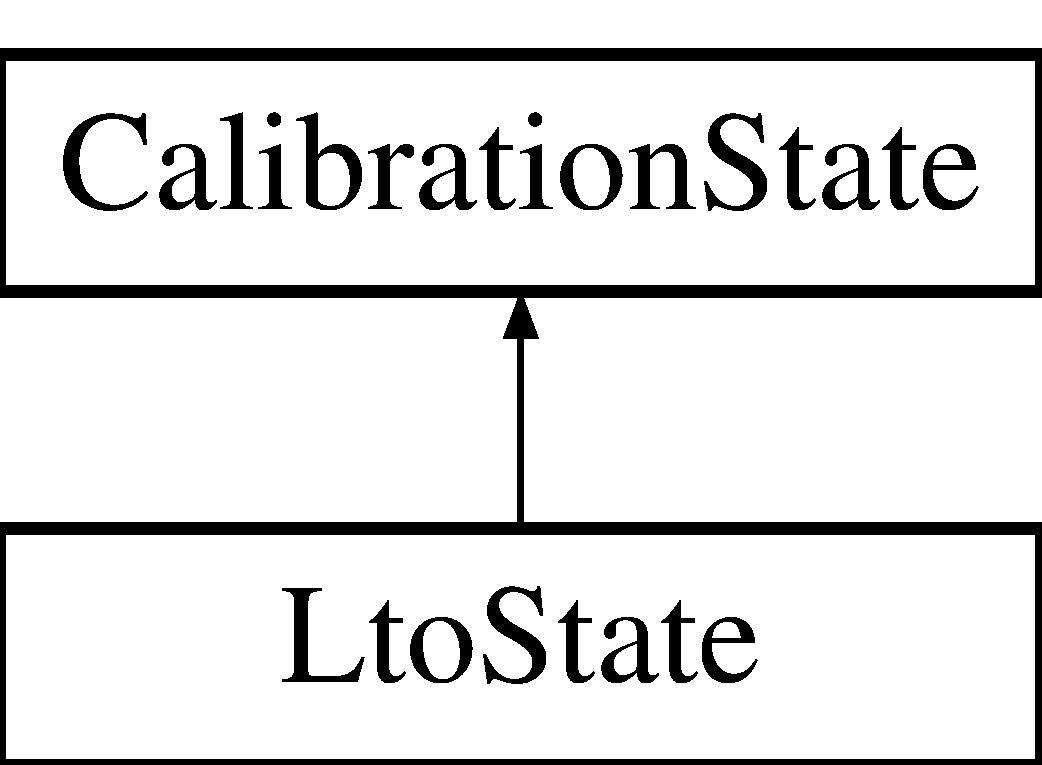
\includegraphics[height=2.000000cm]{classLtoState}
\end{center}
\end{figure}
\subsection*{\-Public \-Member \-Functions}
\begin{DoxyCompactItemize}
\item 
\hypertarget{classLtoState_ac65f1437c32321adae036a236e8e7518}{bool {\bfseries is\-Better\-Than} (const \hyperlink{classLtoState}{\-Lto\-State} other)}\label{classLtoState_ac65f1437c32321adae036a236e8e7518}

\end{DoxyCompactItemize}
\subsection*{\-Public \-Attributes}
\begin{DoxyCompactItemize}
\item 
\hypertarget{classLtoState_a792b3fe57dc114e874423d91ada33bc5}{double {\bfseries error}}\label{classLtoState_a792b3fe57dc114e874423d91ada33bc5}

\end{DoxyCompactItemize}
\subsection*{\-Friends}
\begin{DoxyCompactItemize}
\item 
\hypertarget{classLtoState_a1e00afe1953a5ecdede47a1a77bb0aff}{std\-::ostream \& {\bfseries operator$<$$<$} (std\-::ostream \&out, \hyperlink{classLtoState}{\-Lto\-State} \&state)}\label{classLtoState_a1e00afe1953a5ecdede47a1a77bb0aff}

\end{DoxyCompactItemize}


\-The documentation for this class was generated from the following file\-:\begin{DoxyCompactItemize}
\item 
/home/stefan/catkin\-\_\-ws/src/calibration/include/\-Local\-Transform\-Optimization.\-h\end{DoxyCompactItemize}

\hypertarget{classManualTransformFactory}{\section{\-Manual\-Transform\-Factory \-Class \-Reference}
\label{classManualTransformFactory}\index{\-Manual\-Transform\-Factory@{\-Manual\-Transform\-Factory}}
}


{\ttfamily \#include $<$\-Transform\-Factory.\-h$>$}

\-Inheritance diagram for \-Manual\-Transform\-Factory\-:\begin{figure}[H]
\begin{center}
\leavevmode
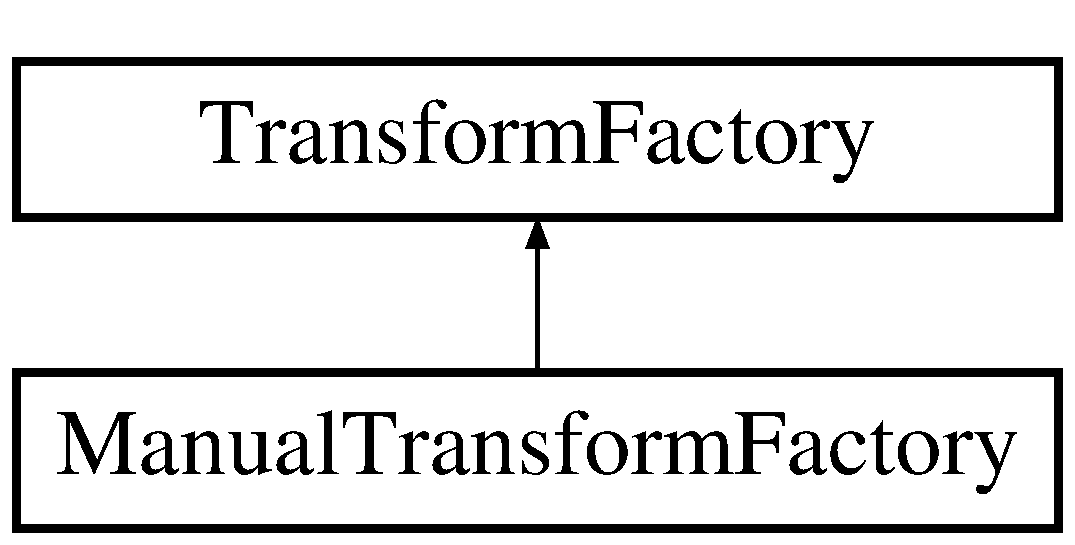
\includegraphics[height=2.000000cm]{classManualTransformFactory}
\end{center}
\end{figure}
\subsection*{\-Public \-Member \-Functions}
\begin{DoxyCompactItemize}
\item 
\hypertarget{classManualTransformFactory_afc411062d26d5d88f6563016a292b940}{{\bfseries \-Manual\-Transform\-Factory} (float tx, float ty, float tz, float roll, float pitch, float yaw)}\label{classManualTransformFactory_afc411062d26d5d88f6563016a292b940}

\item 
\hypertarget{classManualTransformFactory_a3df3685278325ed40137a353b590a1b1}{{\bfseries \-Manual\-Transform\-Factory} (tf\-::\-Transform t)}\label{classManualTransformFactory_a3df3685278325ed40137a353b590a1b1}

\item 
\hypertarget{classManualTransformFactory_a9684b70631ae69eca554ad6e0c8986f4}{virtual void {\bfseries get\-Transform} (tf\-::\-Transform \&transform)}\label{classManualTransformFactory_a9684b70631ae69eca554ad6e0c8986f4}

\end{DoxyCompactItemize}
\subsection*{\-Protected \-Attributes}
\begin{DoxyCompactItemize}
\item 
\hypertarget{classManualTransformFactory_a291e5ff15ef05e7fc236c264c2438f0d}{tf\-::\-Transform {\bfseries transform}}\label{classManualTransformFactory_a291e5ff15ef05e7fc236c264c2438f0d}

\end{DoxyCompactItemize}


\subsection{\-Detailed \-Description}
\-Gets the transform from input. 

\-The documentation for this class was generated from the following files\-:\begin{DoxyCompactItemize}
\item 
/home/stefan/catkin\-\_\-ws/src/calibration/include/\-Transform\-Factory.\-h\item 
/home/stefan/catkin\-\_\-ws/src/calibration/src/\-Transform\-Factory.\-cpp\end{DoxyCompactItemize}

\hypertarget{classMarkerEstimation}{\section{\-Marker\-Estimation \-Class \-Reference}
\label{classMarkerEstimation}\index{\-Marker\-Estimation@{\-Marker\-Estimation}}
}
\subsection*{\-Public \-Member \-Functions}
\begin{DoxyCompactItemize}
\item 
\hypertarget{classMarkerEstimation_ae1e6badeba63e866b606b907985c17b2}{{\bfseries \-Marker\-Estimation} (const std\-::vector$<$ \hyperlink{classCameraMeasurePoint}{\-Measure\-Point} $>$ \&points)}\label{classMarkerEstimation_ae1e6badeba63e866b606b907985c17b2}

\item 
\hypertarget{classMarkerEstimation_a6c5c3ee310f9f2f5a27b88f1e2cf3d1b}{\-Eigen\-::\-Vector3d {\bfseries estimate\-Marker\-Position} (const \hyperlink{classCalibrationState}{\-Calibration\-State} state) const }\label{classMarkerEstimation_a6c5c3ee310f9f2f5a27b88f1e2cf3d1b}

\end{DoxyCompactItemize}
\subsection*{\-Protected \-Attributes}
\begin{DoxyCompactItemize}
\item 
\hypertarget{classMarkerEstimation_ab2ded828c72d1ef198861cbf5c999581}{const std\-::vector$<$ \hyperlink{classCameraMeasurePoint}{\-Measure\-Point} $>$ \& {\bfseries points}}\label{classMarkerEstimation_ab2ded828c72d1ef198861cbf5c999581}

\end{DoxyCompactItemize}


\-The documentation for this class was generated from the following files\-:\begin{DoxyCompactItemize}
\item 
/home/stefan/catkin\-\_\-ws/src/calibration/include/\-Marker\-Estimation.\-h\item 
/home/stefan/catkin\-\_\-ws/src/calibration/src/\-Marker\-Estimation.\-cpp\end{DoxyCompactItemize}

\hypertarget{classOptimizationInstanceBuilder}{\section{\-Optimization\-Instance\-Builder \-Class \-Reference}
\label{classOptimizationInstanceBuilder}\index{\-Optimization\-Instance\-Builder@{\-Optimization\-Instance\-Builder}}
}
\subsection*{\-Static \-Public \-Member \-Functions}
\begin{DoxyCompactItemize}
\item 
\hypertarget{classOptimizationInstanceBuilder_ab7768f462e7e3b67f32fdad8efbf17d7}{static \*
\hyperlink{classCameraTransformOptimization}{\-Camera\-Transform\-Optimization} $\ast$ {\bfseries get\-Instance} (const \hyperlink{classCameraTransformOptimizationParameter}{\-Camera\-Transform\-Optimization\-Parameter} \&param)}\label{classOptimizationInstanceBuilder_ab7768f462e7e3b67f32fdad8efbf17d7}

\item 
\hypertarget{classOptimizationInstanceBuilder_afb2f36a23c0360dbc1388441acbba2ac}{static \*
\hyperlink{classCameraTransformOptimization}{\-Camera\-Transform\-Optimization} $\ast$ {\bfseries get\-Instance} (const std\-::vector$<$ \hyperlink{classCameraTransformOptimizationParameter}{\-Camera\-Transform\-Optimization\-Parameter} $>$ \&params)}\label{classOptimizationInstanceBuilder_afb2f36a23c0360dbc1388441acbba2ac}

\end{DoxyCompactItemize}


\-The documentation for this class was generated from the following files\-:\begin{DoxyCompactItemize}
\item 
/home/stefan/catkin\-\_\-ws/src/calibration/include/\-Optimization\-Instance\-Builder.\-h\item 
/home/stefan/catkin\-\_\-ws/src/calibration/src/\-Optimization\-Instance\-Builder.\-cpp\end{DoxyCompactItemize}

\hypertarget{classParameterAccess}{\section{\-Parameter\-Access \-Class \-Reference}
\label{classParameterAccess}\index{\-Parameter\-Access@{\-Parameter\-Access}}
}
\-Inheritance diagram for \-Parameter\-Access\-:\begin{figure}[H]
\begin{center}
\leavevmode
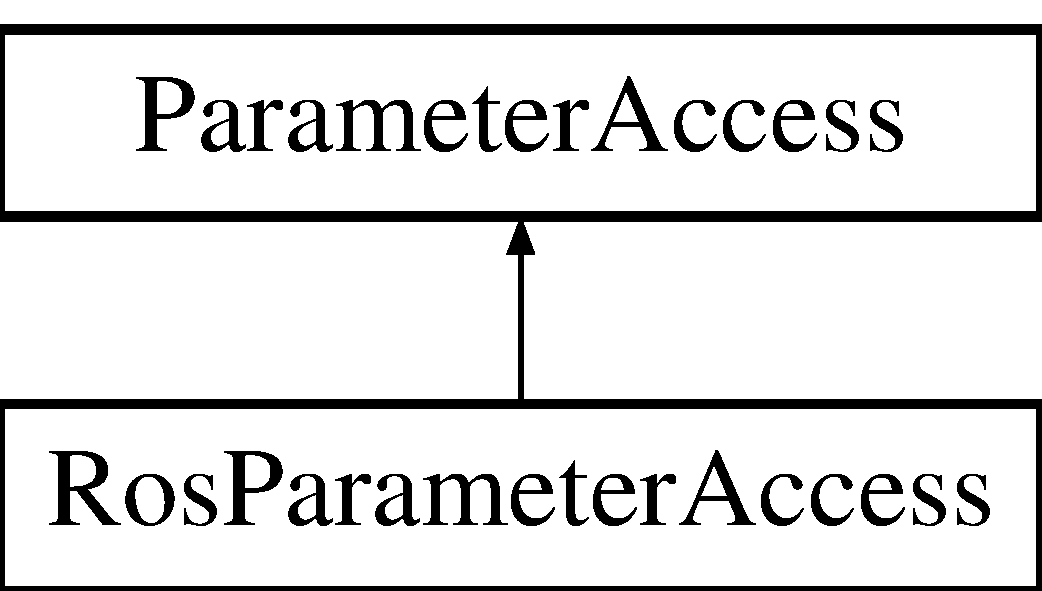
\includegraphics[height=2.000000cm]{classParameterAccess}
\end{center}
\end{figure}
\subsection*{\-Public \-Member \-Functions}
\begin{DoxyCompactItemize}
\item 
\hypertarget{classParameterAccess_adf4c641e72e4cf2cf85c161e62141695}{virtual \hyperlink{classBallDetectionParameter}{\-Ball\-Detection\-Parameter} {\bfseries get\-Ball\-Detection\-Parameter} ()=0}\label{classParameterAccess_adf4c641e72e4cf2cf85c161e62141695}

\item 
\hypertarget{classParameterAccess_ac2afa16de939099c0501eb20167dbac6}{virtual \hyperlink{classDataCaptureParameter}{\-Data\-Capture\-Parameter} {\bfseries get\-Data\-Capture\-Parameter} ()=0}\label{classParameterAccess_ac2afa16de939099c0501eb20167dbac6}

\item 
\hypertarget{classParameterAccess_a367559bb83e49df23ff0310d7fa0c1c2}{virtual std\-::vector\*
$<$ \hyperlink{classCameraTransformOptimizationParameter}{\-Camera\-Transform\-Optimization\-Parameter} $>$ {\bfseries get\-Camera\-Transform\-Optimization\-Parameter} ()=0}\label{classParameterAccess_a367559bb83e49df23ff0310d7fa0c1c2}

\item 
\hypertarget{classParameterAccess_a2445da8bfe762d221490e456d72130e4}{\hyperlink{classCameraCalibrationOptions}{\-Camera\-Calibration\-Options} {\bfseries get\-Camera\-Calibration\-Options} ()}\label{classParameterAccess_a2445da8bfe762d221490e456d72130e4}

\end{DoxyCompactItemize}


\-The documentation for this class was generated from the following files\-:\begin{DoxyCompactItemize}
\item 
/home/stefan/catkin\-\_\-ws/src/calibration/include/\-Parameter\-Access.\-h\item 
/home/stefan/catkin\-\_\-ws/src/calibration/src/\-Parameter\-Access.\-cpp\end{DoxyCompactItemize}

\hypertarget{classParameterAccessFactory}{\section{\-Parameter\-Access\-Factory \-Class \-Reference}
\label{classParameterAccessFactory}\index{\-Parameter\-Access\-Factory@{\-Parameter\-Access\-Factory}}
}
\subsection*{\-Static \-Public \-Member \-Functions}
\begin{DoxyCompactItemize}
\item 
\hypertarget{classParameterAccessFactory_a8b1ca357bc753557bcd2372f9c17eee4}{static \hyperlink{classRosParameterAccess}{\-Ros\-Parameter\-Access} \& {\bfseries get\-Rosparam\-Instance} ()}\label{classParameterAccessFactory_a8b1ca357bc753557bcd2372f9c17eee4}

\end{DoxyCompactItemize}


\-The documentation for this class was generated from the following file\-:\begin{DoxyCompactItemize}
\item 
/home/stefan/catkin\-\_\-ws/src/calibration/include/\-Parameter\-Access.\-h\end{DoxyCompactItemize}

\hypertarget{classRandomRestartLocalOptimization}{\section{\-Random\-Restart\-Local\-Optimization \-Class \-Reference}
\label{classRandomRestartLocalOptimization}\index{\-Random\-Restart\-Local\-Optimization@{\-Random\-Restart\-Local\-Optimization}}
}
\-Inheritance diagram for \-Random\-Restart\-Local\-Optimization\-:\begin{figure}[H]
\begin{center}
\leavevmode
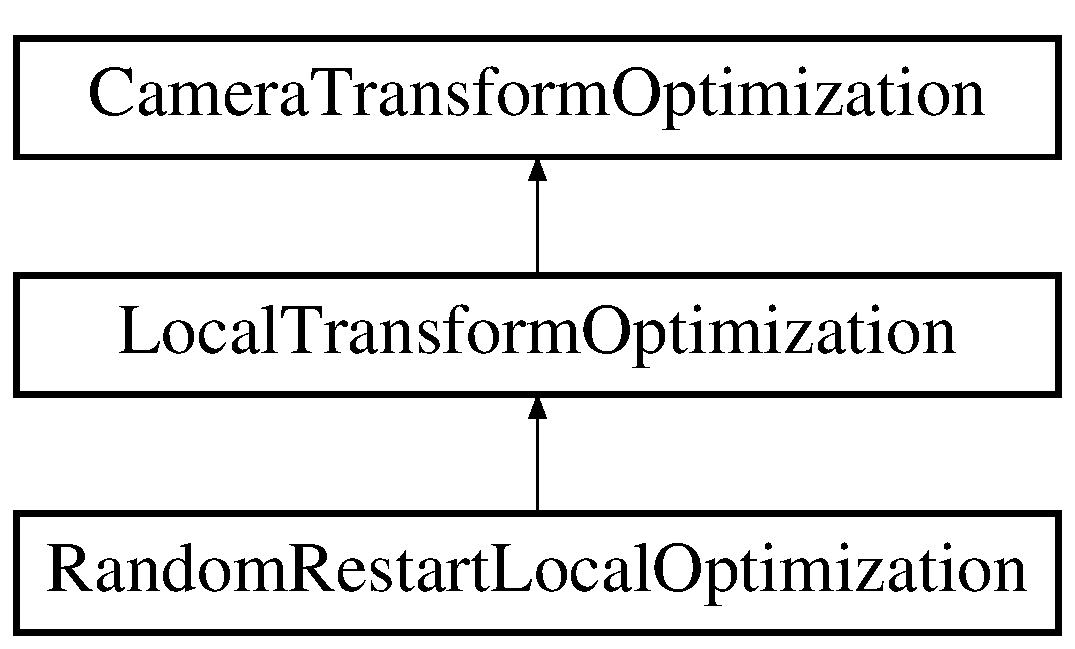
\includegraphics[height=3.000000cm]{classRandomRestartLocalOptimization}
\end{center}
\end{figure}
\subsection*{\-Public \-Member \-Functions}
\begin{DoxyCompactItemize}
\item 
\hypertarget{classRandomRestartLocalOptimization_a54dd1d298dfbe907561947a2d0a707cf}{{\bfseries \-Random\-Restart\-Local\-Optimization} (\hyperlink{classLocalTransformOptimization}{\-Local\-Transform\-Optimization} $\ast$algorithm, int num\-Of\-Restarts)}\label{classRandomRestartLocalOptimization_a54dd1d298dfbe907561947a2d0a707cf}

\item 
virtual void \hyperlink{classRandomRestartLocalOptimization_a6e5936d8717ed841becb50c1f04ee388}{optimize\-Transform} (\hyperlink{classCalibrationState}{\-Calibration\-State} \&calibration\-State)
\end{DoxyCompactItemize}
\subsection*{\-Protected \-Member \-Functions}
\begin{DoxyCompactItemize}
\item 
\hypertarget{classRandomRestartLocalOptimization_ab1f05a0784715b172217af54a934be14}{virtual void {\bfseries get\-Random\-State} (\hyperlink{classLtoState}{\-Lto\-State} \&random\-State)}\label{classRandomRestartLocalOptimization_ab1f05a0784715b172217af54a934be14}

\end{DoxyCompactItemize}


\subsection{\-Member \-Function \-Documentation}
\hypertarget{classRandomRestartLocalOptimization_a6e5936d8717ed841becb50c1f04ee388}{\index{\-Random\-Restart\-Local\-Optimization@{\-Random\-Restart\-Local\-Optimization}!optimize\-Transform@{optimize\-Transform}}
\index{optimize\-Transform@{optimize\-Transform}!RandomRestartLocalOptimization@{\-Random\-Restart\-Local\-Optimization}}
\subsubsection[{optimize\-Transform}]{\setlength{\rightskip}{0pt plus 5cm}void {\bf \-Random\-Restart\-Local\-Optimization\-::optimize\-Transform} (
\begin{DoxyParamCaption}
\item[{{\bf \-Calibration\-State} \&}]{calibration\-State}
\end{DoxyParamCaption}
)\hspace{0.3cm}{\ttfamily  \mbox{[}virtual\mbox{]}}}}\label{classRandomRestartLocalOptimization_a6e5936d8717ed841becb50c1f04ee388}
\-Optimizes the transform given the measured points, initial transformation, and all other transformations needed. 

\-Implements \hyperlink{classCameraTransformOptimization_a8a4a4a09325f4bae401bad62ec7e9f02}{\-Camera\-Transform\-Optimization}.



\-The documentation for this class was generated from the following files\-:\begin{DoxyCompactItemize}
\item 
/home/stefan/catkin\-\_\-ws/src/calibration/include/\-Local\-Transform\-Optimization.\-h\item 
/home/stefan/catkin\-\_\-ws/src/calibration/src/\-Local\-Transform\-Optimization.\-cpp\end{DoxyCompactItemize}

\hypertarget{classRosParameterAccess}{\section{\-Ros\-Parameter\-Access \-Class \-Reference}
\label{classRosParameterAccess}\index{\-Ros\-Parameter\-Access@{\-Ros\-Parameter\-Access}}
}
\-Inheritance diagram for \-Ros\-Parameter\-Access\-:\begin{figure}[H]
\begin{center}
\leavevmode
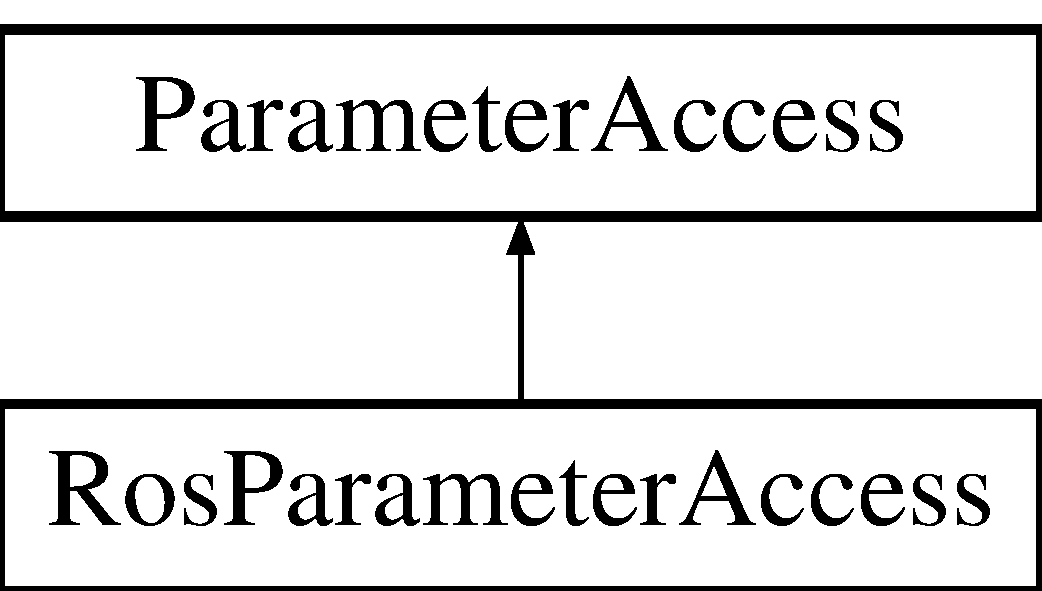
\includegraphics[height=2.000000cm]{classRosParameterAccess}
\end{center}
\end{figure}
\subsection*{\-Public \-Member \-Functions}
\begin{DoxyCompactItemize}
\item 
\hypertarget{classRosParameterAccess_aeed78ae357b863caf91a9065cbcf85ad}{virtual \hyperlink{classBallDetectionParameter}{\-Ball\-Detection\-Parameter} {\bfseries get\-Ball\-Detection\-Parameter} ()}\label{classRosParameterAccess_aeed78ae357b863caf91a9065cbcf85ad}

\item 
\hypertarget{classRosParameterAccess_a556f2a0983a33f1f03b564985082f144}{virtual \hyperlink{classDataCaptureParameter}{\-Data\-Capture\-Parameter} {\bfseries get\-Data\-Capture\-Parameter} ()}\label{classRosParameterAccess_a556f2a0983a33f1f03b564985082f144}

\item 
\hypertarget{classRosParameterAccess_a0c93727c44a5b85de35f62610e6d30a1}{virtual std\-::vector\*
$<$ \hyperlink{classCameraTransformOptimizationParameter}{\-Camera\-Transform\-Optimization\-Parameter} $>$ {\bfseries get\-Camera\-Transform\-Optimization\-Parameter} ()}\label{classRosParameterAccess_a0c93727c44a5b85de35f62610e6d30a1}

\end{DoxyCompactItemize}
\subsection*{\-Static \-Public \-Member \-Functions}
\begin{DoxyCompactItemize}
\item 
\hypertarget{classRosParameterAccess_a6e39677fa574dda712bc2eb7a19a65fb}{static \hyperlink{classRosParameterAccess}{\-Ros\-Parameter\-Access} \& {\bfseries get\-Instance} ()}\label{classRosParameterAccess_a6e39677fa574dda712bc2eb7a19a65fb}

\end{DoxyCompactItemize}


\-The documentation for this class was generated from the following files\-:\begin{DoxyCompactItemize}
\item 
/home/stefan/catkin\-\_\-ws/src/calibration/include/\-Parameter\-Access.\-h\item 
/home/stefan/catkin\-\_\-ws/src/calibration/src/\-Parameter\-Access.\-cpp\end{DoxyCompactItemize}

\hypertarget{classSimulatedAnnealingTransformOptimization}{\section{\-Simulated\-Annealing\-Transform\-Optimization \-Class \-Reference}
\label{classSimulatedAnnealingTransformOptimization}\index{\-Simulated\-Annealing\-Transform\-Optimization@{\-Simulated\-Annealing\-Transform\-Optimization}}
}
\-Inheritance diagram for \-Simulated\-Annealing\-Transform\-Optimization\-:\begin{figure}[H]
\begin{center}
\leavevmode
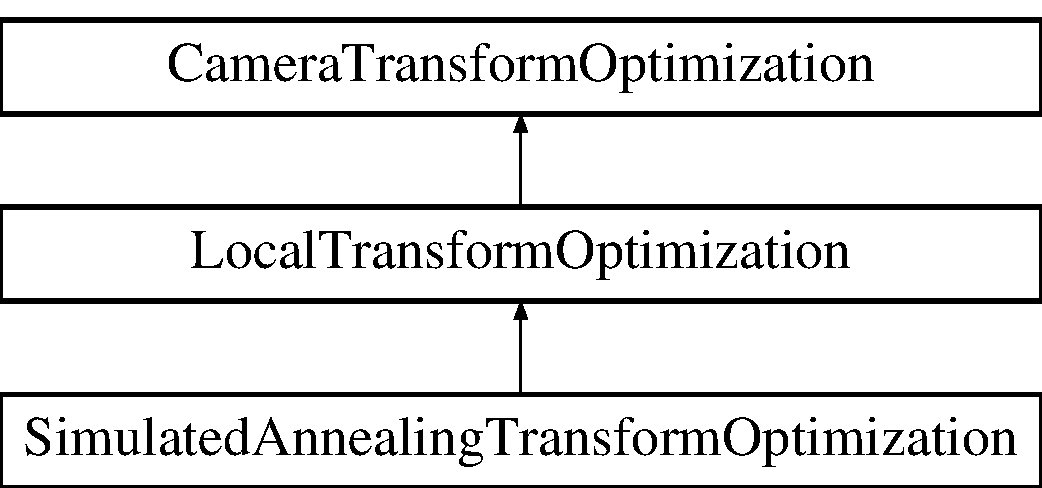
\includegraphics[height=3.000000cm]{classSimulatedAnnealingTransformOptimization}
\end{center}
\end{figure}
\subsection*{\-Public \-Member \-Functions}
\begin{DoxyCompactItemize}
\item 
\hypertarget{classSimulatedAnnealingTransformOptimization_a7cfecf67ac1750612ea38d7d26b884db}{{\bfseries \-Simulated\-Annealing\-Transform\-Optimization} (\hyperlink{classCameraTransformOptimizationParameter}{\-Camera\-Transform\-Optimization\-Parameter} parameter=\hyperlink{classCameraTransformOptimizationParameter}{\-Camera\-Transform\-Optimization\-Parameter}())}\label{classSimulatedAnnealingTransformOptimization_a7cfecf67ac1750612ea38d7d26b884db}

\item 
virtual void \hyperlink{classSimulatedAnnealingTransformOptimization_ab6690824306f9cd1f98f420a8d85e0f7}{optimize\-Transform} (\hyperlink{classCalibrationState}{\-Calibration\-State} \&calibration\-State)
\item 
\hypertarget{classSimulatedAnnealingTransformOptimization_a345f3cfb53e0f1f9512032f6523d1a20}{virtual std\-::vector$<$ \hyperlink{classLtoState}{\-Lto\-State} $>$ {\bfseries get\-Neighbors} (\hyperlink{classLtoState}{\-Lto\-State} \&current)}\label{classSimulatedAnnealingTransformOptimization_a345f3cfb53e0f1f9512032f6523d1a20}

\end{DoxyCompactItemize}
\subsection*{\-Protected \-Attributes}
\begin{DoxyCompactItemize}
\item 
\hypertarget{classSimulatedAnnealingTransformOptimization_a743945c03481f93fd775ac8928f91a17}{float {\bfseries start\-Temperature}}\label{classSimulatedAnnealingTransformOptimization_a743945c03481f93fd775ac8928f91a17}

\end{DoxyCompactItemize}


\subsection{\-Member \-Function \-Documentation}
\hypertarget{classSimulatedAnnealingTransformOptimization_ab6690824306f9cd1f98f420a8d85e0f7}{\index{\-Simulated\-Annealing\-Transform\-Optimization@{\-Simulated\-Annealing\-Transform\-Optimization}!optimize\-Transform@{optimize\-Transform}}
\index{optimize\-Transform@{optimize\-Transform}!SimulatedAnnealingTransformOptimization@{\-Simulated\-Annealing\-Transform\-Optimization}}
\subsubsection[{optimize\-Transform}]{\setlength{\rightskip}{0pt plus 5cm}void {\bf \-Simulated\-Annealing\-Transform\-Optimization\-::optimize\-Transform} (
\begin{DoxyParamCaption}
\item[{{\bf \-Calibration\-State} \&}]{calibration\-State}
\end{DoxyParamCaption}
)\hspace{0.3cm}{\ttfamily  \mbox{[}virtual\mbox{]}}}}\label{classSimulatedAnnealingTransformOptimization_ab6690824306f9cd1f98f420a8d85e0f7}
\-Optimizes the transform given the measured points, initial transformation, and all other transformations needed. 

\-Implements \hyperlink{classCameraTransformOptimization_a8a4a4a09325f4bae401bad62ec7e9f02}{\-Camera\-Transform\-Optimization}.



\-The documentation for this class was generated from the following files\-:\begin{DoxyCompactItemize}
\item 
/home/stefan/catkin\-\_\-ws/src/calibration/include/\-Local\-Transform\-Optimization.\-h\item 
/home/stefan/catkin\-\_\-ws/src/calibration/src/\-Local\-Transform\-Optimization.\-cpp\end{DoxyCompactItemize}

\hypertarget{classSvdTransformOptimization}{\section{\-Svd\-Transform\-Optimization \-Class \-Reference}
\label{classSvdTransformOptimization}\index{\-Svd\-Transform\-Optimization@{\-Svd\-Transform\-Optimization}}
}
\-Inheritance diagram for \-Svd\-Transform\-Optimization\-:\begin{figure}[H]
\begin{center}
\leavevmode
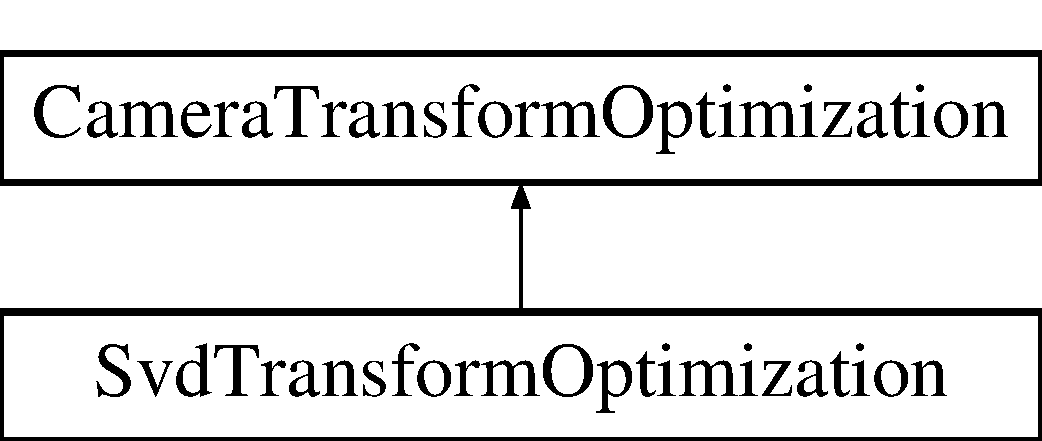
\includegraphics[height=2.000000cm]{classSvdTransformOptimization}
\end{center}
\end{figure}
\subsection*{\-Public \-Member \-Functions}
\begin{DoxyCompactItemize}
\item 
\hypertarget{classSvdTransformOptimization_a51a90a884290d5898a27dcb8cbb12980}{{\bfseries \-Svd\-Transform\-Optimization} (\hyperlink{classCameraTransformOptimizationParameter}{\-Camera\-Transform\-Optimization\-Parameter} parameter=\hyperlink{classCameraTransformOptimizationParameter}{\-Camera\-Transform\-Optimization\-Parameter}())}\label{classSvdTransformOptimization_a51a90a884290d5898a27dcb8cbb12980}

\item 
virtual void \hyperlink{classSvdTransformOptimization_afd4d0ed3de6c59535ede1f06134463e8}{optimize\-Transform} (\hyperlink{classCalibrationState}{\-Calibration\-State} \&calibration\-State)
\end{DoxyCompactItemize}


\subsection{\-Member \-Function \-Documentation}
\hypertarget{classSvdTransformOptimization_afd4d0ed3de6c59535ede1f06134463e8}{\index{\-Svd\-Transform\-Optimization@{\-Svd\-Transform\-Optimization}!optimize\-Transform@{optimize\-Transform}}
\index{optimize\-Transform@{optimize\-Transform}!SvdTransformOptimization@{\-Svd\-Transform\-Optimization}}
\subsubsection[{optimize\-Transform}]{\setlength{\rightskip}{0pt plus 5cm}void {\bf \-Svd\-Transform\-Optimization\-::optimize\-Transform} (
\begin{DoxyParamCaption}
\item[{{\bf \-Calibration\-State} \&}]{calibration\-State}
\end{DoxyParamCaption}
)\hspace{0.3cm}{\ttfamily  \mbox{[}virtual\mbox{]}}}}\label{classSvdTransformOptimization_afd4d0ed3de6c59535ede1f06134463e8}
\-Optimizes the transform given the measured points, initial transformation, and all other transformations needed. 

\-Implements \hyperlink{classCameraTransformOptimization_a8a4a4a09325f4bae401bad62ec7e9f02}{\-Camera\-Transform\-Optimization}.



\-The documentation for this class was generated from the following files\-:\begin{DoxyCompactItemize}
\item 
/home/stefan/catkin\-\_\-ws/src/calibration/include/\-Svd\-Transform\-Optimization.\-h\item 
/home/stefan/catkin\-\_\-ws/src/calibration/src/\-Svd\-Transform\-Optimization.\-cpp\end{DoxyCompactItemize}

\hypertarget{classTfTransformFactory}{\section{\-Tf\-Transform\-Factory \-Class \-Reference}
\label{classTfTransformFactory}\index{\-Tf\-Transform\-Factory@{\-Tf\-Transform\-Factory}}
}


{\ttfamily \#include $<$\-Transform\-Factory.\-h$>$}

\-Inheritance diagram for \-Tf\-Transform\-Factory\-:\begin{figure}[H]
\begin{center}
\leavevmode
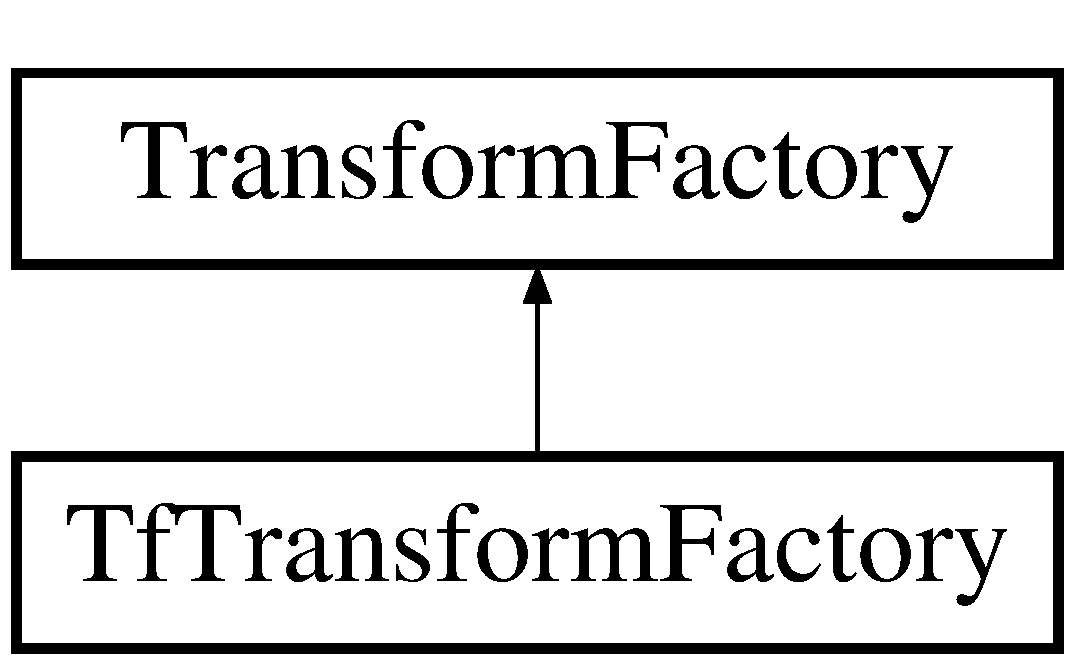
\includegraphics[height=2.000000cm]{classTfTransformFactory}
\end{center}
\end{figure}
\subsection*{\-Public \-Member \-Functions}
\begin{DoxyCompactItemize}
\item 
\hypertarget{classTfTransformFactory_a64ad5f97558fff2a1ac9fc9f6a1e7195}{{\bfseries \-Tf\-Transform\-Factory} (std\-::string target\-Frame, std\-::string source\-Frame)}\label{classTfTransformFactory_a64ad5f97558fff2a1ac9fc9f6a1e7195}

\item 
\hypertarget{classTfTransformFactory_afbf08c88d042160b83fe6b5ad3592ac2}{virtual void {\bfseries get\-Transform} (tf\-::\-Transform \&transform)}\label{classTfTransformFactory_afbf08c88d042160b83fe6b5ad3592ac2}

\end{DoxyCompactItemize}
\subsection*{\-Protected \-Attributes}
\begin{DoxyCompactItemize}
\item 
\hypertarget{classTfTransformFactory_afa2716e228add9788cc3063f40632cc9}{std\-::string {\bfseries target\-Frame}}\label{classTfTransformFactory_afa2716e228add9788cc3063f40632cc9}

\item 
\hypertarget{classTfTransformFactory_a1d39f491b56155e0e02b1a90f47c8879}{std\-::string {\bfseries source\-Frame}}\label{classTfTransformFactory_a1d39f491b56155e0e02b1a90f47c8879}

\item 
\hypertarget{classTfTransformFactory_a39f386acdb290de27c686ce08072c974}{tf\-::\-Transform\-Listener {\bfseries transform\-Listener}}\label{classTfTransformFactory_a39f386acdb290de27c686ce08072c974}

\end{DoxyCompactItemize}


\subsection{\-Detailed \-Description}
\-Gets the transform from \-T\-F. 

\-The documentation for this class was generated from the following files\-:\begin{DoxyCompactItemize}
\item 
/home/stefan/catkin\-\_\-ws/src/calibration/include/\-Transform\-Factory.\-h\item 
/home/stefan/catkin\-\_\-ws/src/calibration/src/\-Transform\-Factory.\-cpp\end{DoxyCompactItemize}

\hypertarget{classTransformFactory}{\section{\-Transform\-Factory \-Class \-Reference}
\label{classTransformFactory}\index{\-Transform\-Factory@{\-Transform\-Factory}}
}


{\ttfamily \#include $<$\-Transform\-Factory.\-h$>$}

\-Inheritance diagram for \-Transform\-Factory\-:\begin{figure}[H]
\begin{center}
\leavevmode
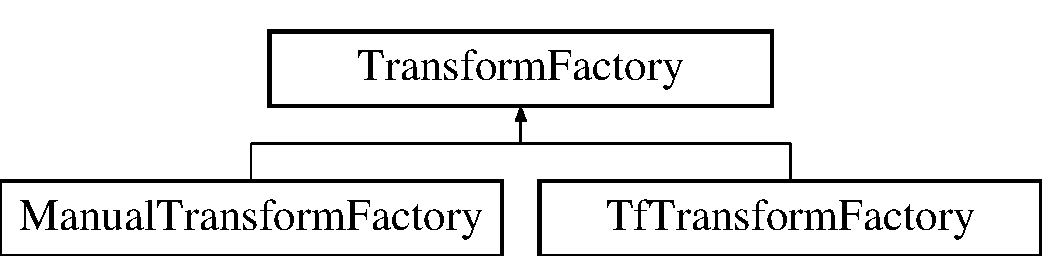
\includegraphics[height=2.000000cm]{classTransformFactory}
\end{center}
\end{figure}
\subsection*{\-Public \-Member \-Functions}
\begin{DoxyCompactItemize}
\item 
\hypertarget{classTransformFactory_a649ac11e65ef023dbbddb4c4a971a109}{virtual void {\bfseries get\-Transform} (tf\-::\-Transform \&transform)=0}\label{classTransformFactory_a649ac11e65ef023dbbddb4c4a971a109}

\end{DoxyCompactItemize}


\subsection{\-Detailed \-Description}
\-Class for getting a transform. 

\-The documentation for this class was generated from the following files\-:\begin{DoxyCompactItemize}
\item 
/home/stefan/catkin\-\_\-ws/src/calibration/include/\-Transform\-Factory.\-h\item 
/home/stefan/catkin\-\_\-ws/src/calibration/src/\-Transform\-Factory.\-cpp\end{DoxyCompactItemize}

\hypertarget{classVertexOffset}{\section{\-Vertex\-Offset \-Class \-Reference}
\label{classVertexOffset}\index{\-Vertex\-Offset@{\-Vertex\-Offset}}
}
\subsection*{\-Public \-Member \-Functions}
\begin{DoxyCompactItemize}
\item 
\hypertarget{classVertexOffset_a273b4799e4290018314da16c83201230}{virtual bool {\bfseries read} (std\-::istream \&)}\label{classVertexOffset_a273b4799e4290018314da16c83201230}

\item 
\hypertarget{classVertexOffset_a4bf3ce6bec4f351a3f9270982d733a97}{virtual bool {\bfseries write} (std\-::ostream \&) const }\label{classVertexOffset_a4bf3ce6bec4f351a3f9270982d733a97}

\item 
\hypertarget{classVertexOffset_a6e697d722e9e160c19347931786b77cc}{virtual void {\bfseries oplus\-Impl} (const double $\ast$)}\label{classVertexOffset_a6e697d722e9e160c19347931786b77cc}

\item 
\hypertarget{classVertexOffset_a62e82a4d29bb226c12633f5d98a6b2b7}{virtual void {\bfseries set\-To\-Origin\-Impl} ()}\label{classVertexOffset_a62e82a4d29bb226c12633f5d98a6b2b7}

\end{DoxyCompactItemize}


\-The documentation for this class was generated from the following files\-:\begin{DoxyCompactItemize}
\item 
/home/stefan/catkin\-\_\-ws/src/calibration/include/\-Vertex\-Offset.\-h\item 
/home/stefan/catkin\-\_\-ws/src/calibration/src/\-Vertex\-Offset.\-cpp\end{DoxyCompactItemize}

\hypertarget{classVertexPosition3D}{\section{\-Vertex\-Position3\-D \-Class \-Reference}
\label{classVertexPosition3D}\index{\-Vertex\-Position3\-D@{\-Vertex\-Position3\-D}}
}
\subsection*{\-Public \-Member \-Functions}
\begin{DoxyCompactItemize}
\item 
\hypertarget{classVertexPosition3D_ab2901f62bab0c224e95a0e7f10c006ef}{virtual bool {\bfseries read} (std\-::istream \&)}\label{classVertexPosition3D_ab2901f62bab0c224e95a0e7f10c006ef}

\item 
\hypertarget{classVertexPosition3D_a6a9c429663ed1eb568b894a3d2f83f5b}{virtual bool {\bfseries write} (std\-::ostream \&) const }\label{classVertexPosition3D_a6a9c429663ed1eb568b894a3d2f83f5b}

\item 
\hypertarget{classVertexPosition3D_a11a4b6772e02a44203ad0fb824449d8e}{virtual void {\bfseries oplus\-Impl} (const double $\ast$)}\label{classVertexPosition3D_a11a4b6772e02a44203ad0fb824449d8e}

\item 
\hypertarget{classVertexPosition3D_af904c5967e9e4dd53282206c62491faf}{virtual void {\bfseries set\-To\-Origin\-Impl} ()}\label{classVertexPosition3D_af904c5967e9e4dd53282206c62491faf}

\item 
\hypertarget{classVertexPosition3D_a0aa22b03e0c190abdb695f8eb2a09892}{\-Eigen\-::\-Vector3d {\bfseries estimate\-Marker\-Position} (const \hyperlink{classCalibrationState}{\-Calibration\-State} state) const }\label{classVertexPosition3D_a0aa22b03e0c190abdb695f8eb2a09892}

\end{DoxyCompactItemize}


\-The documentation for this class was generated from the following files\-:\begin{DoxyCompactItemize}
\item 
/home/stefan/catkin\-\_\-ws/src/calibration/include/\-Vertex\-Position3\-D.\-h\item 
/home/stefan/catkin\-\_\-ws/src/calibration/src/\-Vertex\-Position3\-D.\-cpp\end{DoxyCompactItemize}

\hypertarget{classVertexTransformation3D}{\section{\-Vertex\-Transformation3\-D \-Class \-Reference}
\label{classVertexTransformation3D}\index{\-Vertex\-Transformation3\-D@{\-Vertex\-Transformation3\-D}}
}
\subsection*{\-Public \-Member \-Functions}
\begin{DoxyCompactItemize}
\item 
\hypertarget{classVertexTransformation3D_a27cbcba13590e4d1985813d6f4f43d9f}{virtual bool {\bfseries read} (std\-::istream \&in)}\label{classVertexTransformation3D_a27cbcba13590e4d1985813d6f4f43d9f}

\item 
\hypertarget{classVertexTransformation3D_a0aa1f47af0ced2ced081b2dfe8533fd9}{virtual bool {\bfseries write} (std\-::ostream \&out) const }\label{classVertexTransformation3D_a0aa1f47af0ced2ced081b2dfe8533fd9}

\item 
\hypertarget{classVertexTransformation3D_a86bd4cf36cb0bfa652357e4d2ca958f3}{virtual void {\bfseries oplus\-Impl} (const double $\ast$)}\label{classVertexTransformation3D_a86bd4cf36cb0bfa652357e4d2ca958f3}

\item 
\hypertarget{classVertexTransformation3D_a03f2a8897a5e859728b94a5495dcce4d}{virtual void {\bfseries set\-To\-Origin\-Impl} ()}\label{classVertexTransformation3D_a03f2a8897a5e859728b94a5495dcce4d}

\end{DoxyCompactItemize}


\-The documentation for this class was generated from the following files\-:\begin{DoxyCompactItemize}
\item 
/home/stefan/catkin\-\_\-ws/src/calibration/include/\-Vertex\-Transformation3\-D.\-h\item 
/home/stefan/catkin\-\_\-ws/src/calibration/src/\-Vertex\-Transformation3\-D.\-cpp\end{DoxyCompactItemize}

\printindex
\end{document}
